\documentclass[11pt]{article}
    \usepackage{ctex}
    \usepackage[breakable]{tcolorbox}
    \usepackage{parskip} % Stop auto-indenting (to mimic markdown behaviour)
    
    \usepackage{iftex}
    \ifPDFTeX
    	\usepackage[T1]{fontenc}
    	\usepackage{mathpazo}
    \else
    	\usepackage{fontspec}
    \fi

    % Basic figure setup, for now with no caption control since it's done
    % automatically by Pandoc (which extracts ![](path) syntax from Markdown).
    \usepackage{graphicx}
    % Maintain compatibility with old templates. Remove in nbconvert 6.0
    \let\Oldincludegraphics\includegraphics
    % Ensure that by default, figures have no caption (until we provide a
    % proper Figure object with a Caption API and a way to capture that
    % in the conversion process - todo).
    \usepackage{caption}
    \DeclareCaptionFormat{nocaption}{}
    \captionsetup{format=nocaption,aboveskip=0pt,belowskip=0pt}

    \usepackage[Export]{adjustbox} % Used to constrain images to a maximum size
    \adjustboxset{max size={0.9\linewidth}{0.9\paperheight}}
    \usepackage{float}
    \floatplacement{figure}{H} % forces figures to be placed at the correct location
    \usepackage{xcolor} % Allow colors to be defined
    \usepackage{enumerate} % Needed for markdown enumerations to work
    \usepackage{geometry} % Used to adjust the document margins
    \usepackage{amsmath} % Equations
    \usepackage{amssymb} % Equations
    \usepackage{textcomp} % defines textquotesingle
    % Hack from http://tex.stackexchange.com/a/47451/13684:
    \AtBeginDocument{%
        \def\PYZsq{\textquotesingle}% Upright quotes in Pygmentized code
    }
    \usepackage{upquote} % Upright quotes for verbatim code
    \usepackage{eurosym} % defines \euro
    \usepackage[mathletters]{ucs} % Extended unicode (utf-8) support
    \usepackage{fancyvrb} % verbatim replacement that allows latex
    \usepackage{grffile} % extends the file name processing of package graphics 
                         % to support a larger range
    \makeatletter % fix for grffile with XeLaTeX
    \def\Gread@@xetex#1{%
      \IfFileExists{"\Gin@base".bb}%
      {\Gread@eps{\Gin@base.bb}}%
      {\Gread@@xetex@aux#1}%
    }
    \makeatother

    % The hyperref package gives us a pdf with properly built
    % internal navigation ('pdf bookmarks' for the table of contents,
    % internal cross-reference links, web links for URLs, etc.)
    \usepackage{hyperref}
    % The default LaTeX title has an obnoxious amount of whitespace. By default,
    % titling removes some of it. It also provides customization options.
    \usepackage{titling}
    \usepackage{longtable} % longtable support required by pandoc >1.10
    \usepackage{booktabs}  % table support for pandoc > 1.12.2
    \usepackage[inline]{enumitem} % IRkernel/repr support (it uses the enumerate* environment)
    \usepackage[normalem]{ulem} % ulem is needed to support strikethroughs (\sout)
                                % normalem makes italics be italics, not underlines
    \usepackage{mathrsfs}
    

    
    % Colors for the hyperref package
    \definecolor{urlcolor}{rgb}{0,.145,.698}
    \definecolor{linkcolor}{rgb}{.71,0.21,0.01}
    \definecolor{citecolor}{rgb}{.12,.54,.11}

    % ANSI colors
    \definecolor{ansi-black}{HTML}{3E424D}
    \definecolor{ansi-black-intense}{HTML}{282C36}
    \definecolor{ansi-red}{HTML}{E75C58}
    \definecolor{ansi-red-intense}{HTML}{B22B31}
    \definecolor{ansi-green}{HTML}{00A250}
    \definecolor{ansi-green-intense}{HTML}{007427}
    \definecolor{ansi-yellow}{HTML}{DDB62B}
    \definecolor{ansi-yellow-intense}{HTML}{B27D12}
    \definecolor{ansi-blue}{HTML}{208FFB}
    \definecolor{ansi-blue-intense}{HTML}{0065CA}
    \definecolor{ansi-magenta}{HTML}{D160C4}
    \definecolor{ansi-magenta-intense}{HTML}{A03196}
    \definecolor{ansi-cyan}{HTML}{60C6C8}
    \definecolor{ansi-cyan-intense}{HTML}{258F8F}
    \definecolor{ansi-white}{HTML}{C5C1B4}
    \definecolor{ansi-white-intense}{HTML}{A1A6B2}
    \definecolor{ansi-default-inverse-fg}{HTML}{FFFFFF}
    \definecolor{ansi-default-inverse-bg}{HTML}{000000}

    % commands and environments needed by pandoc snippets
    % extracted from the output of `pandoc -s`
    \providecommand{\tightlist}{%
      \setlength{\itemsep}{0pt}\setlength{\parskip}{0pt}}
    \DefineVerbatimEnvironment{Highlighting}{Verbatim}{commandchars=\\\{\}}
    % Add ',fontsize=\small' for more characters per line
    \newenvironment{Shaded}{}{}
    \newcommand{\KeywordTok}[1]{\textcolor[rgb]{0.00,0.44,0.13}{\textbf{{#1}}}}
    \newcommand{\DataTypeTok}[1]{\textcolor[rgb]{0.56,0.13,0.00}{{#1}}}
    \newcommand{\DecValTok}[1]{\textcolor[rgb]{0.25,0.63,0.44}{{#1}}}
    \newcommand{\BaseNTok}[1]{\textcolor[rgb]{0.25,0.63,0.44}{{#1}}}
    \newcommand{\FloatTok}[1]{\textcolor[rgb]{0.25,0.63,0.44}{{#1}}}
    \newcommand{\CharTok}[1]{\textcolor[rgb]{0.25,0.44,0.63}{{#1}}}
    \newcommand{\StringTok}[1]{\textcolor[rgb]{0.25,0.44,0.63}{{#1}}}
    \newcommand{\CommentTok}[1]{\textcolor[rgb]{0.38,0.63,0.69}{\textit{{#1}}}}
    \newcommand{\OtherTok}[1]{\textcolor[rgb]{0.00,0.44,0.13}{{#1}}}
    \newcommand{\AlertTok}[1]{\textcolor[rgb]{1.00,0.00,0.00}{\textbf{{#1}}}}
    \newcommand{\FunctionTok}[1]{\textcolor[rgb]{0.02,0.16,0.49}{{#1}}}
    \newcommand{\RegionMarkerTok}[1]{{#1}}
    \newcommand{\ErrorTok}[1]{\textcolor[rgb]{1.00,0.00,0.00}{\textbf{{#1}}}}
    \newcommand{\NormalTok}[1]{{#1}}
    
    % Additional commands for more recent versions of Pandoc
    \newcommand{\ConstantTok}[1]{\textcolor[rgb]{0.53,0.00,0.00}{{#1}}}
    \newcommand{\SpecialCharTok}[1]{\textcolor[rgb]{0.25,0.44,0.63}{{#1}}}
    \newcommand{\VerbatimStringTok}[1]{\textcolor[rgb]{0.25,0.44,0.63}{{#1}}}
    \newcommand{\SpecialStringTok}[1]{\textcolor[rgb]{0.73,0.40,0.53}{{#1}}}
    \newcommand{\ImportTok}[1]{{#1}}
    \newcommand{\DocumentationTok}[1]{\textcolor[rgb]{0.73,0.13,0.13}{\textit{{#1}}}}
    \newcommand{\AnnotationTok}[1]{\textcolor[rgb]{0.38,0.63,0.69}{\textbf{\textit{{#1}}}}}
    \newcommand{\CommentVarTok}[1]{\textcolor[rgb]{0.38,0.63,0.69}{\textbf{\textit{{#1}}}}}
    \newcommand{\VariableTok}[1]{\textcolor[rgb]{0.10,0.09,0.49}{{#1}}}
    \newcommand{\ControlFlowTok}[1]{\textcolor[rgb]{0.00,0.44,0.13}{\textbf{{#1}}}}
    \newcommand{\OperatorTok}[1]{\textcolor[rgb]{0.40,0.40,0.40}{{#1}}}
    \newcommand{\BuiltInTok}[1]{{#1}}
    \newcommand{\ExtensionTok}[1]{{#1}}
    \newcommand{\PreprocessorTok}[1]{\textcolor[rgb]{0.74,0.48,0.00}{{#1}}}
    \newcommand{\AttributeTok}[1]{\textcolor[rgb]{0.49,0.56,0.16}{{#1}}}
    \newcommand{\InformationTok}[1]{\textcolor[rgb]{0.38,0.63,0.69}{\textbf{\textit{{#1}}}}}
    \newcommand{\WarningTok}[1]{\textcolor[rgb]{0.38,0.63,0.69}{\textbf{\textit{{#1}}}}}
    
    
    % Define a nice break command that doesn't care if a line doesn't already
    % exist.
    \def\br{\hspace*{\fill} \\* }
    % Math Jax compatibility definitions
    \def\gt{>}
    \def\lt{<}
    \let\Oldtex\TeX
    \let\Oldlatex\LaTeX
    \renewcommand{\TeX}{\textrm{\Oldtex}}
    \renewcommand{\LaTeX}{\textrm{\Oldlatex}}
    % Document parameters
    % Document title
    \title{lecture03}
    \author{Zeffiretti Hieah}
    
    
    
    
    
% Pygments definitions
\makeatletter
\def\PY@reset{\let\PY@it=\relax \let\PY@bf=\relax%
    \let\PY@ul=\relax \let\PY@tc=\relax%
    \let\PY@bc=\relax \let\PY@ff=\relax}
\def\PY@tok#1{\csname PY@tok@#1\endcsname}
\def\PY@toks#1+{\ifx\relax#1\empty\else%
    \PY@tok{#1}\expandafter\PY@toks\fi}
\def\PY@do#1{\PY@bc{\PY@tc{\PY@ul{%
    \PY@it{\PY@bf{\PY@ff{#1}}}}}}}
\def\PY#1#2{\PY@reset\PY@toks#1+\relax+\PY@do{#2}}

\expandafter\def\csname PY@tok@w\endcsname{\def\PY@tc##1{\textcolor[rgb]{0.73,0.73,0.73}{##1}}}
\expandafter\def\csname PY@tok@c\endcsname{\let\PY@it=\textit\def\PY@tc##1{\textcolor[rgb]{0.25,0.50,0.50}{##1}}}
\expandafter\def\csname PY@tok@cp\endcsname{\def\PY@tc##1{\textcolor[rgb]{0.74,0.48,0.00}{##1}}}
\expandafter\def\csname PY@tok@k\endcsname{\let\PY@bf=\textbf\def\PY@tc##1{\textcolor[rgb]{0.00,0.50,0.00}{##1}}}
\expandafter\def\csname PY@tok@kp\endcsname{\def\PY@tc##1{\textcolor[rgb]{0.00,0.50,0.00}{##1}}}
\expandafter\def\csname PY@tok@kt\endcsname{\def\PY@tc##1{\textcolor[rgb]{0.69,0.00,0.25}{##1}}}
\expandafter\def\csname PY@tok@o\endcsname{\def\PY@tc##1{\textcolor[rgb]{0.40,0.40,0.40}{##1}}}
\expandafter\def\csname PY@tok@ow\endcsname{\let\PY@bf=\textbf\def\PY@tc##1{\textcolor[rgb]{0.67,0.13,1.00}{##1}}}
\expandafter\def\csname PY@tok@nb\endcsname{\def\PY@tc##1{\textcolor[rgb]{0.00,0.50,0.00}{##1}}}
\expandafter\def\csname PY@tok@nf\endcsname{\def\PY@tc##1{\textcolor[rgb]{0.00,0.00,1.00}{##1}}}
\expandafter\def\csname PY@tok@nc\endcsname{\let\PY@bf=\textbf\def\PY@tc##1{\textcolor[rgb]{0.00,0.00,1.00}{##1}}}
\expandafter\def\csname PY@tok@nn\endcsname{\let\PY@bf=\textbf\def\PY@tc##1{\textcolor[rgb]{0.00,0.00,1.00}{##1}}}
\expandafter\def\csname PY@tok@ne\endcsname{\let\PY@bf=\textbf\def\PY@tc##1{\textcolor[rgb]{0.82,0.25,0.23}{##1}}}
\expandafter\def\csname PY@tok@nv\endcsname{\def\PY@tc##1{\textcolor[rgb]{0.10,0.09,0.49}{##1}}}
\expandafter\def\csname PY@tok@no\endcsname{\def\PY@tc##1{\textcolor[rgb]{0.53,0.00,0.00}{##1}}}
\expandafter\def\csname PY@tok@nl\endcsname{\def\PY@tc##1{\textcolor[rgb]{0.63,0.63,0.00}{##1}}}
\expandafter\def\csname PY@tok@ni\endcsname{\let\PY@bf=\textbf\def\PY@tc##1{\textcolor[rgb]{0.60,0.60,0.60}{##1}}}
\expandafter\def\csname PY@tok@na\endcsname{\def\PY@tc##1{\textcolor[rgb]{0.49,0.56,0.16}{##1}}}
\expandafter\def\csname PY@tok@nt\endcsname{\let\PY@bf=\textbf\def\PY@tc##1{\textcolor[rgb]{0.00,0.50,0.00}{##1}}}
\expandafter\def\csname PY@tok@nd\endcsname{\def\PY@tc##1{\textcolor[rgb]{0.67,0.13,1.00}{##1}}}
\expandafter\def\csname PY@tok@s\endcsname{\def\PY@tc##1{\textcolor[rgb]{0.73,0.13,0.13}{##1}}}
\expandafter\def\csname PY@tok@sd\endcsname{\let\PY@it=\textit\def\PY@tc##1{\textcolor[rgb]{0.73,0.13,0.13}{##1}}}
\expandafter\def\csname PY@tok@si\endcsname{\let\PY@bf=\textbf\def\PY@tc##1{\textcolor[rgb]{0.73,0.40,0.53}{##1}}}
\expandafter\def\csname PY@tok@se\endcsname{\let\PY@bf=\textbf\def\PY@tc##1{\textcolor[rgb]{0.73,0.40,0.13}{##1}}}
\expandafter\def\csname PY@tok@sr\endcsname{\def\PY@tc##1{\textcolor[rgb]{0.73,0.40,0.53}{##1}}}
\expandafter\def\csname PY@tok@ss\endcsname{\def\PY@tc##1{\textcolor[rgb]{0.10,0.09,0.49}{##1}}}
\expandafter\def\csname PY@tok@sx\endcsname{\def\PY@tc##1{\textcolor[rgb]{0.00,0.50,0.00}{##1}}}
\expandafter\def\csname PY@tok@m\endcsname{\def\PY@tc##1{\textcolor[rgb]{0.40,0.40,0.40}{##1}}}
\expandafter\def\csname PY@tok@gh\endcsname{\let\PY@bf=\textbf\def\PY@tc##1{\textcolor[rgb]{0.00,0.00,0.50}{##1}}}
\expandafter\def\csname PY@tok@gu\endcsname{\let\PY@bf=\textbf\def\PY@tc##1{\textcolor[rgb]{0.50,0.00,0.50}{##1}}}
\expandafter\def\csname PY@tok@gd\endcsname{\def\PY@tc##1{\textcolor[rgb]{0.63,0.00,0.00}{##1}}}
\expandafter\def\csname PY@tok@gi\endcsname{\def\PY@tc##1{\textcolor[rgb]{0.00,0.63,0.00}{##1}}}
\expandafter\def\csname PY@tok@gr\endcsname{\def\PY@tc##1{\textcolor[rgb]{1.00,0.00,0.00}{##1}}}
\expandafter\def\csname PY@tok@ge\endcsname{\let\PY@it=\textit}
\expandafter\def\csname PY@tok@gs\endcsname{\let\PY@bf=\textbf}
\expandafter\def\csname PY@tok@gp\endcsname{\let\PY@bf=\textbf\def\PY@tc##1{\textcolor[rgb]{0.00,0.00,0.50}{##1}}}
\expandafter\def\csname PY@tok@go\endcsname{\def\PY@tc##1{\textcolor[rgb]{0.53,0.53,0.53}{##1}}}
\expandafter\def\csname PY@tok@gt\endcsname{\def\PY@tc##1{\textcolor[rgb]{0.00,0.27,0.87}{##1}}}
\expandafter\def\csname PY@tok@err\endcsname{\def\PY@bc##1{\setlength{\fboxsep}{0pt}\fcolorbox[rgb]{1.00,0.00,0.00}{1,1,1}{\strut ##1}}}
\expandafter\def\csname PY@tok@kc\endcsname{\let\PY@bf=\textbf\def\PY@tc##1{\textcolor[rgb]{0.00,0.50,0.00}{##1}}}
\expandafter\def\csname PY@tok@kd\endcsname{\let\PY@bf=\textbf\def\PY@tc##1{\textcolor[rgb]{0.00,0.50,0.00}{##1}}}
\expandafter\def\csname PY@tok@kn\endcsname{\let\PY@bf=\textbf\def\PY@tc##1{\textcolor[rgb]{0.00,0.50,0.00}{##1}}}
\expandafter\def\csname PY@tok@kr\endcsname{\let\PY@bf=\textbf\def\PY@tc##1{\textcolor[rgb]{0.00,0.50,0.00}{##1}}}
\expandafter\def\csname PY@tok@bp\endcsname{\def\PY@tc##1{\textcolor[rgb]{0.00,0.50,0.00}{##1}}}
\expandafter\def\csname PY@tok@fm\endcsname{\def\PY@tc##1{\textcolor[rgb]{0.00,0.00,1.00}{##1}}}
\expandafter\def\csname PY@tok@vc\endcsname{\def\PY@tc##1{\textcolor[rgb]{0.10,0.09,0.49}{##1}}}
\expandafter\def\csname PY@tok@vg\endcsname{\def\PY@tc##1{\textcolor[rgb]{0.10,0.09,0.49}{##1}}}
\expandafter\def\csname PY@tok@vi\endcsname{\def\PY@tc##1{\textcolor[rgb]{0.10,0.09,0.49}{##1}}}
\expandafter\def\csname PY@tok@vm\endcsname{\def\PY@tc##1{\textcolor[rgb]{0.10,0.09,0.49}{##1}}}
\expandafter\def\csname PY@tok@sa\endcsname{\def\PY@tc##1{\textcolor[rgb]{0.73,0.13,0.13}{##1}}}
\expandafter\def\csname PY@tok@sb\endcsname{\def\PY@tc##1{\textcolor[rgb]{0.73,0.13,0.13}{##1}}}
\expandafter\def\csname PY@tok@sc\endcsname{\def\PY@tc##1{\textcolor[rgb]{0.73,0.13,0.13}{##1}}}
\expandafter\def\csname PY@tok@dl\endcsname{\def\PY@tc##1{\textcolor[rgb]{0.73,0.13,0.13}{##1}}}
\expandafter\def\csname PY@tok@s2\endcsname{\def\PY@tc##1{\textcolor[rgb]{0.73,0.13,0.13}{##1}}}
\expandafter\def\csname PY@tok@sh\endcsname{\def\PY@tc##1{\textcolor[rgb]{0.73,0.13,0.13}{##1}}}
\expandafter\def\csname PY@tok@s1\endcsname{\def\PY@tc##1{\textcolor[rgb]{0.73,0.13,0.13}{##1}}}
\expandafter\def\csname PY@tok@mb\endcsname{\def\PY@tc##1{\textcolor[rgb]{0.40,0.40,0.40}{##1}}}
\expandafter\def\csname PY@tok@mf\endcsname{\def\PY@tc##1{\textcolor[rgb]{0.40,0.40,0.40}{##1}}}
\expandafter\def\csname PY@tok@mh\endcsname{\def\PY@tc##1{\textcolor[rgb]{0.40,0.40,0.40}{##1}}}
\expandafter\def\csname PY@tok@mi\endcsname{\def\PY@tc##1{\textcolor[rgb]{0.40,0.40,0.40}{##1}}}
\expandafter\def\csname PY@tok@il\endcsname{\def\PY@tc##1{\textcolor[rgb]{0.40,0.40,0.40}{##1}}}
\expandafter\def\csname PY@tok@mo\endcsname{\def\PY@tc##1{\textcolor[rgb]{0.40,0.40,0.40}{##1}}}
\expandafter\def\csname PY@tok@ch\endcsname{\let\PY@it=\textit\def\PY@tc##1{\textcolor[rgb]{0.25,0.50,0.50}{##1}}}
\expandafter\def\csname PY@tok@cm\endcsname{\let\PY@it=\textit\def\PY@tc##1{\textcolor[rgb]{0.25,0.50,0.50}{##1}}}
\expandafter\def\csname PY@tok@cpf\endcsname{\let\PY@it=\textit\def\PY@tc##1{\textcolor[rgb]{0.25,0.50,0.50}{##1}}}
\expandafter\def\csname PY@tok@c1\endcsname{\let\PY@it=\textit\def\PY@tc##1{\textcolor[rgb]{0.25,0.50,0.50}{##1}}}
\expandafter\def\csname PY@tok@cs\endcsname{\let\PY@it=\textit\def\PY@tc##1{\textcolor[rgb]{0.25,0.50,0.50}{##1}}}

\def\PYZbs{\char`\\}
\def\PYZus{\char`\_}
\def\PYZob{\char`\{}
\def\PYZcb{\char`\}}
\def\PYZca{\char`\^}
\def\PYZam{\char`\&}
\def\PYZlt{\char`\<}
\def\PYZgt{\char`\>}
\def\PYZsh{\char`\#}
\def\PYZpc{\char`\%}
\def\PYZdl{\char`\$}
\def\PYZhy{\char`\-}
\def\PYZsq{\char`\'}
\def\PYZdq{\char`\"}
\def\PYZti{\char`\~}
% for compatibility with earlier versions
\def\PYZat{@}
\def\PYZlb{[}
\def\PYZrb{]}
\makeatother


    % For linebreaks inside Verbatim environment from package fancyvrb. 
    \makeatletter
        \newbox\Wrappedcontinuationbox 
        \newbox\Wrappedvisiblespacebox 
        \newcommand*\Wrappedvisiblespace {\textcolor{red}{\textvisiblespace}} 
        \newcommand*\Wrappedcontinuationsymbol {\textcolor{red}{\llap{\tiny$\m@th\hookrightarrow$}}} 
        \newcommand*\Wrappedcontinuationindent {3ex } 
        \newcommand*\Wrappedafterbreak {\kern\Wrappedcontinuationindent\copy\Wrappedcontinuationbox} 
        % Take advantage of the already applied Pygments mark-up to insert 
        % potential linebreaks for TeX processing. 
        %        {, <, #, %, $, ' and ": go to next line. 
        %        _, }, ^, &, >, - and ~: stay at end of broken line. 
        % Use of \textquotesingle for straight quote. 
        \newcommand*\Wrappedbreaksatspecials {% 
            \def\PYGZus{\discretionary{\char`\_}{\Wrappedafterbreak}{\char`\_}}% 
            \def\PYGZob{\discretionary{}{\Wrappedafterbreak\char`\{}{\char`\{}}% 
            \def\PYGZcb{\discretionary{\char`\}}{\Wrappedafterbreak}{\char`\}}}% 
            \def\PYGZca{\discretionary{\char`\^}{\Wrappedafterbreak}{\char`\^}}% 
            \def\PYGZam{\discretionary{\char`\&}{\Wrappedafterbreak}{\char`\&}}% 
            \def\PYGZlt{\discretionary{}{\Wrappedafterbreak\char`\<}{\char`\<}}% 
            \def\PYGZgt{\discretionary{\char`\>}{\Wrappedafterbreak}{\char`\>}}% 
            \def\PYGZsh{\discretionary{}{\Wrappedafterbreak\char`\#}{\char`\#}}% 
            \def\PYGZpc{\discretionary{}{\Wrappedafterbreak\char`\%}{\char`\%}}% 
            \def\PYGZdl{\discretionary{}{\Wrappedafterbreak\char`\$}{\char`\$}}% 
            \def\PYGZhy{\discretionary{\char`\-}{\Wrappedafterbreak}{\char`\-}}% 
            \def\PYGZsq{\discretionary{}{\Wrappedafterbreak\textquotesingle}{\textquotesingle}}% 
            \def\PYGZdq{\discretionary{}{\Wrappedafterbreak\char`\"}{\char`\"}}% 
            \def\PYGZti{\discretionary{\char`\~}{\Wrappedafterbreak}{\char`\~}}% 
        } 
        % Some characters . , ; ? ! / are not pygmentized. 
        % This macro makes them "active" and they will insert potential linebreaks 
        \newcommand*\Wrappedbreaksatpunct {% 
            \lccode`\~`\.\lowercase{\def~}{\discretionary{\hbox{\char`\.}}{\Wrappedafterbreak}{\hbox{\char`\.}}}% 
            \lccode`\~`\,\lowercase{\def~}{\discretionary{\hbox{\char`\,}}{\Wrappedafterbreak}{\hbox{\char`\,}}}% 
            \lccode`\~`\;\lowercase{\def~}{\discretionary{\hbox{\char`\;}}{\Wrappedafterbreak}{\hbox{\char`\;}}}% 
            \lccode`\~`\:\lowercase{\def~}{\discretionary{\hbox{\char`\:}}{\Wrappedafterbreak}{\hbox{\char`\:}}}% 
            \lccode`\~`\?\lowercase{\def~}{\discretionary{\hbox{\char`\?}}{\Wrappedafterbreak}{\hbox{\char`\?}}}% 
            \lccode`\~`\!\lowercase{\def~}{\discretionary{\hbox{\char`\!}}{\Wrappedafterbreak}{\hbox{\char`\!}}}% 
            \lccode`\~`\/\lowercase{\def~}{\discretionary{\hbox{\char`\/}}{\Wrappedafterbreak}{\hbox{\char`\/}}}% 
            \catcode`\.\active
            \catcode`\,\active 
            \catcode`\;\active
            \catcode`\:\active
            \catcode`\?\active
            \catcode`\!\active
            \catcode`\/\active 
            \lccode`\~`\~ 	
        }
    \makeatother

    \let\OriginalVerbatim=\Verbatim
    \makeatletter
    \renewcommand{\Verbatim}[1][1]{%
        %\parskip\z@skip
        \sbox\Wrappedcontinuationbox {\Wrappedcontinuationsymbol}%
        \sbox\Wrappedvisiblespacebox {\FV@SetupFont\Wrappedvisiblespace}%
        \def\FancyVerbFormatLine ##1{\hsize\linewidth
            \vtop{\raggedright\hyphenpenalty\z@\exhyphenpenalty\z@
                \doublehyphendemerits\z@\finalhyphendemerits\z@
                \strut ##1\strut}%
        }%
        % If the linebreak is at a space, the latter will be displayed as visible
        % space at end of first line, and a continuation symbol starts next line.
        % Stretch/shrink are however usually zero for typewriter font.
        \def\FV@Space {%
            \nobreak\hskip\z@ plus\fontdimen3\font minus\fontdimen4\font
            \discretionary{\copy\Wrappedvisiblespacebox}{\Wrappedafterbreak}
            {\kern\fontdimen2\font}%
        }%
        
        % Allow breaks at special characters using \PYG... macros.
        \Wrappedbreaksatspecials
        % Breaks at punctuation characters . , ; ? ! and / need catcode=\active 	
        \OriginalVerbatim[#1,codes*=\Wrappedbreaksatpunct]%
    }
    \makeatother

    % Exact colors from NB
    \definecolor{incolor}{HTML}{303F9F}
    \definecolor{outcolor}{HTML}{D84315}
    \definecolor{cellborder}{HTML}{CFCFCF}
    \definecolor{cellbackground}{HTML}{F7F7F7}
    
    % prompt
    \makeatletter
    \newcommand{\boxspacing}{\kern\kvtcb@left@rule\kern\kvtcb@boxsep}
    \makeatother
    \newcommand{\prompt}[4]{
        \ttfamily\llap{{\color{#2}[#3]:\hspace{3pt}#4}}\vspace{-\baselineskip}
    }
    

    
    % Prevent overflowing lines due to hard-to-break entities
    \sloppy 
    % Setup hyperref package
    \hypersetup{
      breaklinks=true,  % so long urls are correctly broken across lines
      colorlinks=true,
      urlcolor=urlcolor,
      linkcolor=linkcolor,
      citecolor=citecolor,
      }
    % Slightly bigger margins than the latex defaults
    
    \geometry{verbose,tmargin=1in,bmargin=1in,lmargin=1in,rmargin=1in}
    
    

\begin{document}
    
    \maketitle
    
    

    
    \hypertarget{basics-of-deformation-elasticity-and-finite-elements}{%
\subsection{Basics of deformation, elasticity, and finite
elements}\label{basics-of-deformation-elasticity-and-finite-elements}}

Simulating of elastic materials is a lot of fun!

\hypertarget{deformation-ux5f62ux53d8}{%
\subsubsection{Deformation (形变)}\label{deformation-ux5f62ux53d8}}

Deformation map \(\phi\): a (vector to vebtor) function that relates
rest material position and deformed material position.

\begin{equation*}
{\rm x_{deformed}}=\phi({\rm x_{rest}})
\end{equation*}

Deformation gradient \({\rm F}\)

\begin{equation*}
{\rm F}:=\displaystyle\frac{\partial{\rm x_{deformed}}}{\partial{\rm x_{rest}}}
\end{equation*}

\emph{Deformation gradients are translational invariant}

\(\phi_{1}=\phi({\rm x_{rest}})\) and
\(\phi_{1}=\phi({\rm x_{rest}})+{\rm c}\) have the same deformation
gradients!

Deform/rest volume ratio \(J=det({\rm F})\)

\hypertarget{hyperelasticityux5f39ux6027}{%
\subsubsection{Hyperelasticity(弹性)}\label{hyperelasticityux5f39ux6027}}

Hyperelasticity materials: materials whose stress-strain relationship is
defined by a \textbf{Strain energy density function(应变能密度函数)}

\begin{equation}
\varPsi = \varPsi({\rm F})
\end{equation}

Intuitive understanding: \(\varPsi\) is a potential function that
penalizes deformation. ``Stress'': the material's internal elastic
forces.(应力) ``Strain'': just replace it with deformation gradients
\({\rm F}\) for now.(应变)

\begin{itemize}
\tightlist
\item
  Be careful We use \(\varPsi\) as the strain energy denisty function
  and \(\phi\) as the deformation map. They are completely
  \textbf{different}.
\end{itemize}

\hypertarget{stress-tensor3times-3ux77e9ux9635}{%
\subsubsection{\texorpdfstring{Stress
Tensor(\(3\times 3\)矩阵)}{Stress Tensor(3\textbackslash times 3矩阵)}}\label{stress-tensor3times-3ux77e9ux9635}}

\textbf{Stress} stands for internal forces that infinitesimal material
components exert on their neighborhood.

Based on our knowledge, we use different measures of \textbf{stress} -
The First Piola-Kirchhoff stress tensor (PK1):
\({\rm P(F)}=\frac{\partial\varPsi({\rm F})}{\partial {\rm F}}\) (easy
to compute, but in rest place) - Kirchhoff stress: \(\tau\) - Cauchy
stress tensor: \(\sigma\) (symmetric, because of conservation of angular
momentum)

Relationship:
\(\tau=J\sigma={\rm PF}^{T}\),\({\rm P}=J\sigma{\rm F}^{-T}\), Traction
\(t=\sigma^{T}{\rm n}\)

\textbf{Intuition of} \({\rm P}=J\sigma{\rm F}^{-T}\): \(J\) compensates
for material compression/expansion. \({\rm F}^{-T}\) compensate for
material deformation. (Note that it's \({\rm F}^{-T}\) instead of
\({\rm F}^{-1}\) since we transform the norm \(\rm n\) instead of
\(\rm x\).)

\hypertarget{elastic-moduli-isotropic-materials}{%
\subsubsection{Elastic moduli (isotropic
materials)}\label{elastic-moduli-isotropic-materials}}

\begin{itemize}
\tightlist
\item
  Youhng's modulus \(E=\displaystyle\frac{\sigma}{\varepsilon}\)
  (杨氏模量)
\item
  Bulk modulus \(K=-V\displaystyle\frac{dP}{dV}\)
  (体积模量,体积弹性系数)
\item
  Poisson's ratio \(\nu\in [0.0,0.5)\) (Auxetics have negative Poisson's
  ratio) (泊松比)
\end{itemize}

\(\rm Lam\acute{e}\)'s modulus: - \(\rm Lam\acute{e}\)'s first paramater
\(\mu\) - \(\rm Lam\acute{e}\)'s second paramater \(\lambda\) (aka.
shear modeulus, denoted by \(G\))

Useful conversion formula:

\begin{equation*}
K=\displaystyle\frac{E}{3(1-2\nu)},\qquad \lambda=\displaystyle\frac{E\nu}{(1+\nu)(1-2\nu)},\qquad \mu=\displaystyle\frac{E}{2(1+\nu)}
\end{equation*}

\hypertarget{hyperelastic-material-models}{%
\subsubsection{Hyperelastic material
models}\label{hyperelastic-material-models}}

Popular ones in graphics: - Linear elasticity (small deformation only) -
Neo-Hookean: -
\(\varPsi({\rm F})=\displaystyle\frac{\mu}{2}\sum_{i}  \left[({\rm F}^{T}{\rm F})_{ii}-1\right]  -\mu{\rm log}(J)+\displaystyle\frac{\lambda}{2}{\rm log}^{2}(J).\)
-
\({\rm P(F)}=\displaystyle\frac{\partial\varPsi({\rm F})}{\partial {\rm F}}  =2\mu({\rm F-R})+\lambda{\rm log}(J){\rm F}^{-T}.\)
- (Fixed) Corotated: -
\(\varPsi({\rm F})=\displaystyle\mu\sum_{i}  (\sigma_{i}-1)^{2}+\displaystyle\frac{\lambda}{2}(J-1)^{2}.\)
\(\sigma_{i}\) are singular values of \({\rm F}.\) -
\({\rm P(F)}=\displaystyle\frac{\partial\varPsi({\rm F})}{\partial {\rm F}}  =2\mu({\rm F-R})+\lambda(J-1)J{\rm F}^{-T}.\)

\hypertarget{the-finite-element-method-ux6709ux9650ux5143}{%
\subsubsection{The finite element method
(有限元)}\label{the-finite-element-method-ux6709ux9650ux5143}}

\textbf{The finite element method:} Galerkin discretization sceme that
builds discrete equations using weak formulations of continuous PDEs.

\begin{figure}
\centering
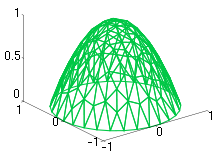
\includegraphics{Finite_element_solution.png}
\caption{A solution to a discretized partial differential equation,
obtained with FEM}
\end{figure}

\hypertarget{linear-tetrahedral-triangular-fem-ux7ebfux6027ux56dbux9762ux4f53ux4e09ux89d2ux5f62ux53d8ux6362}{%
\paragraph{Linear tetrahedral (triangular) FEM
(线性四面体(三角形)变换)}\label{linear-tetrahedral-triangular-fem-ux7ebfux6027ux56dbux9762ux4f53ux4e09ux89d2ux5f62ux53d8ux6362}}

Linear tetrahedral finite elements (for elasticity) asume \textbf{the
deformation map} \(\phi\) \textbf{is affine and thereby deformation
gradient} \({\rm F}\) \textbf{is constant} within a single tetrahedral
element:

\begin{equation*}
{\rm x_{deformed}=Fx_{rest}+b}
\end{equation*}

For every element \(e\), its elastic potential energy

\begin{equation*}
U(e)=\int_{e}\varPsi({\rm F(x)}){\rm x}~d{\rm x}=V_{e}\varPsi({\rm F}_{e})
\end{equation*}

Question: how to compute \({\rm F}_{e}({\rm x})\)? Solution: Recal that
\begin{equation*}
{\rm x_{deformed}=Fx_{rest}+b}
\end{equation*} In 2D triangular elements (3D would be tetrahedral
elemets), assuming the \({\rm rest}\) positions of the vertices (顶点)
are \({\rm a_{rest},b_{rest},c_{rest}}\) and deformed positions are
\({\rm a_{deformed},b_{deformed},c_{deformed}}\). Since within an linear
triangular element \({\rm F}\) is constant, we have

\begin{equation*}
 \begin{array}{rcl}
 {\rm a_{deformed}}&=&{\rm Fa_{rest}+b} \\
 {\rm b_{deformed}}&=&{\rm Fb_{rest}+b} \\
 {\rm c_{deformed}}&=&{\rm Fc_{rest}+b}
 \end{array}
 \end{equation*}

Eliminate \({\rm b}\):

\begin{equation*}
 \begin{array}{rcl}
 {\rm (a_{deformed}-c_{deformed})}&=&{\rm F(a_{rest}-c_{rest})} \\
 {\rm (b_{deformed}-c_{deformed})}&=&{\rm F(b_{rest}-c_{rest})}
 \end{array}
 \end{equation*}

Note that \({\rm F}_{x\times 2}\) now has 4 linear constraints
(equations).

\begin{equation*}
 \begin{array}{rcl}
 {\rm B}&=&{\rm [a_{rest}-c_{rest}|b_{rest}-c_{rest}]}^{-1} \\
 {\rm D}&=&{\rm [a_{deformed}-c_{deformed}|b_{deformed}-c_{deformed}]} \\
 {\rm F}&=&{\rm DB}
 \end{array}
 \end{equation*}

note:\([x|y]\) 代表由\(x\)组成第一列,\(y\)组成第二列的矩阵。

(\(\rm B\) is \emph{constant} through out the physical process.
Therefore it should be pre-computed. \(\rm B\)
是一个常数,因其只与静止状态三角形顶点的位置有关。)

Recall the Semi-implicit Euler (aka. symplectic Euler) time integration.
\begin{equation*}
\begin{array}{rl}
    {\rm v}_ {t+1,i} &= {\rm v}_ {t,i}+\Delta t\displaystyle\frac{{\rm f}_ {t,i}}{m_{i}} \\
    {\rm x}_ {t+1,i} &= {\rm x}_ {t,i}+\Delta t{\rm v}_{t+1,i}
\end{array}
\end{equation*}

Note that \({\rm x}_{t,i}\) and \({\rm v}_{t,i}\) are stored on the
\emph{vertices} of finite elements (triangles/tetrahedrons).

\begin{equation*}
{\rm f}_{t,i}=-\displaystyle\frac{\partial U}{\partial {\rm x}_{i}}
             =-\sum_{e}\frac{\partial U(e)}{\partial {\rm x}_{i}}
             =-\sum_{e}V_{e}\frac{\partial\varPsi({\rm F}_{e})}{\partial{\rm F}_{e}}\frac{\partial{\rm F}_{e}}{\partial {\rm x}_{i}}
             =-\sum_{e}V_{e}{\rm P}({\rm F}_{e})\frac{\partial {\rm F}_{e}}{\partial {\rm x}_{i}}
\end{equation*}

    \begin{tcolorbox}[breakable, size=fbox, boxrule=1pt, pad at break*=1mm,colback=cellbackground, colframe=cellborder]
\prompt{In}{incolor}{1}{\boxspacing}
\begin{Verbatim}[commandchars=\\\{\}]
\PY{k+kn}{import} \PY{n+nn}{taichi} \PY{k}{as} \PY{n+nn}{ti}
\PY{k+kn}{import} \PY{n+nn}{math}

\PY{n}{ti}\PY{o}{.}\PY{n}{init}\PY{p}{(}\PY{n}{arch}\PY{o}{=}\PY{n}{ti}\PY{o}{.}\PY{n}{gpu}\PY{p}{)}

\PY{n}{real} \PY{o}{=} \PY{n}{ti}\PY{o}{.}\PY{n}{f32}
\PY{n}{dim} \PY{o}{=} \PY{l+m+mi}{2}
\PY{n}{n\PYZus{}nodes\PYZus{}x} \PY{o}{=} \PY{l+m+mi}{50}
\PY{n}{n\PYZus{}nodes\PYZus{}y} \PY{o}{=} \PY{l+m+mi}{6}
\PY{n}{node\PYZus{}mass} \PY{o}{=} \PY{l+m+mi}{1}
\PY{n}{n\PYZus{}nodes} \PY{o}{=} \PY{n}{n\PYZus{}nodes\PYZus{}x} \PY{o}{*} \PY{n}{n\PYZus{}nodes\PYZus{}y}
\PY{n}{n\PYZus{}elements} \PY{o}{=} \PY{p}{(}\PY{n}{n\PYZus{}nodes\PYZus{}x} \PY{o}{\PYZhy{}} \PY{l+m+mi}{1}\PY{p}{)} \PY{o}{*} \PY{p}{(}\PY{n}{n\PYZus{}nodes\PYZus{}y} \PY{o}{\PYZhy{}} \PY{l+m+mi}{1}\PY{p}{)} \PY{o}{*} \PY{l+m+mi}{2}
\PY{n}{dt} \PY{o}{=} \PY{l+m+mf}{3e\PYZhy{}4}
\PY{n}{dx} \PY{o}{=} \PY{l+m+mi}{1} \PY{o}{/} \PY{l+m+mi}{32}
\PY{n}{p\PYZus{}mass} \PY{o}{=} \PY{l+m+mi}{1}
\PY{n}{p\PYZus{}vol} \PY{o}{=} \PY{l+m+mi}{1}
\PY{n}{E}\PY{p}{,} \PY{n}{nu} \PY{o}{=} \PY{l+m+mi}{1000}\PY{p}{,} \PY{l+m+mf}{0.3}
\PY{n}{la} \PY{o}{=} \PY{n}{E} \PY{o}{*} \PY{n}{nu} \PY{o}{/} \PY{p}{(}\PY{p}{(}\PY{l+m+mi}{1} \PY{o}{+} \PY{n}{nu}\PY{p}{)} \PY{o}{*} \PY{p}{(}\PY{l+m+mi}{1} \PY{o}{\PYZhy{}} \PY{l+m+mi}{2} \PY{o}{*} \PY{n}{nu}\PY{p}{)}\PY{p}{)}
\PY{n}{mu} \PY{o}{=} \PY{n}{E} \PY{o}{/} \PY{p}{(}\PY{l+m+mi}{2} \PY{o}{*} \PY{p}{(}\PY{l+m+mi}{1} \PY{o}{+} \PY{n}{nu}\PY{p}{)}\PY{p}{)}
\PY{n}{element\PYZus{}V} \PY{o}{=} \PY{l+m+mf}{0.01}

\PY{n}{x} \PY{o}{=} \PY{n}{ti}\PY{o}{.}\PY{n}{Vector}\PY{o}{.}\PY{n}{field}\PY{p}{(}\PY{n}{dim}\PY{p}{,} \PY{n}{dtype}\PY{o}{=}\PY{n}{real}\PY{p}{,} \PY{n}{shape}\PY{o}{=}\PY{n}{n\PYZus{}nodes}\PY{p}{,} \PY{n}{needs\PYZus{}grad}\PY{o}{=}\PY{k+kc}{True}\PY{p}{)}
\PY{n}{v} \PY{o}{=} \PY{n}{ti}\PY{o}{.}\PY{n}{Vector}\PY{o}{.}\PY{n}{field}\PY{p}{(}\PY{n}{dim}\PY{p}{,} \PY{n}{dtype}\PY{o}{=}\PY{n}{real}\PY{p}{,} \PY{n}{shape}\PY{o}{=}\PY{n}{n\PYZus{}nodes}\PY{p}{)}
\PY{n}{B} \PY{o}{=} \PY{n}{ti}\PY{o}{.}\PY{n}{Matrix}\PY{o}{.}\PY{n}{field}\PY{p}{(}\PY{n}{dim}\PY{p}{,} \PY{n}{dim}\PY{p}{,} \PY{n}{dtype}\PY{o}{=}\PY{n}{real}\PY{p}{,} \PY{n}{shape}\PY{o}{=}\PY{n}{n\PYZus{}elements}\PY{p}{)}
\PY{n}{total\PYZus{}energy} \PY{o}{=} \PY{n}{ti}\PY{o}{.}\PY{n}{field}\PY{p}{(}\PY{n}{dtype}\PY{o}{=}\PY{n}{real}\PY{p}{,} \PY{n}{shape}\PY{o}{=}\PY{p}{(}\PY{p}{)}\PY{p}{,} \PY{n}{needs\PYZus{}grad}\PY{o}{=}\PY{k+kc}{True}\PY{p}{)}
\PY{n}{vertices} \PY{o}{=} \PY{n}{ti}\PY{o}{.}\PY{n}{field}\PY{p}{(}\PY{n}{dtype}\PY{o}{=}\PY{n}{ti}\PY{o}{.}\PY{n}{i32}\PY{p}{,} \PY{n}{shape}\PY{o}{=}\PY{p}{(}\PY{n}{n\PYZus{}elements}\PY{p}{,} \PY{l+m+mi}{3}\PY{p}{)}\PY{p}{)}
\PY{n}{sphere} \PY{o}{=} \PY{n}{ti}\PY{o}{.}\PY{n}{Vector}\PY{o}{.}\PY{n}{field}\PY{p}{(}\PY{n}{dim}\PY{p}{,} \PY{n}{dtype}\PY{o}{=}\PY{n}{real}\PY{p}{,} \PY{n}{shape}\PY{o}{=}\PY{p}{(}\PY{p}{)}\PY{p}{)}


\PY{c+c1}{\PYZsh{} print(\PYZdq{}starting...\PYZdq{})}

\PY{n+nd}{@ti}\PY{o}{.}\PY{n}{func}
\PY{k}{def} \PY{n+nf}{compute\PYZus{}D}\PY{p}{(}\PY{n}{i}\PY{p}{)}\PY{p}{:}
    \PY{n}{a} \PY{o}{=} \PY{n}{vertices}\PY{p}{[}\PY{n}{i}\PY{p}{,} \PY{l+m+mi}{0}\PY{p}{]}
    \PY{n}{b} \PY{o}{=} \PY{n}{vertices}\PY{p}{[}\PY{n}{i}\PY{p}{,} \PY{l+m+mi}{1}\PY{p}{]}
    \PY{n}{c} \PY{o}{=} \PY{n}{vertices}\PY{p}{[}\PY{n}{i}\PY{p}{,} \PY{l+m+mi}{2}\PY{p}{]}
    \PY{k}{return} \PY{n}{ti}\PY{o}{.}\PY{n}{Matrix}\PY{o}{.}\PY{n}{cols}\PY{p}{(}\PY{p}{[}\PY{n}{x}\PY{p}{[}\PY{n}{b}\PY{p}{]} \PY{o}{\PYZhy{}} \PY{n}{x}\PY{p}{[}\PY{n}{a}\PY{p}{]}\PY{p}{,} \PY{n}{x}\PY{p}{[}\PY{n}{c}\PY{p}{]} \PY{o}{\PYZhy{}} \PY{n}{x}\PY{p}{[}\PY{n}{a}\PY{p}{]}\PY{p}{]}\PY{p}{)}


\PY{n+nd}{@ti}\PY{o}{.}\PY{n}{kernel}
\PY{k}{def} \PY{n+nf}{compute\PYZus{}B}\PY{p}{(}\PY{p}{)}\PY{p}{:}
    \PY{k}{for} \PY{n}{i} \PY{o+ow}{in} \PY{n+nb}{range}\PY{p}{(}\PY{n}{n\PYZus{}elements}\PY{p}{)}\PY{p}{:}
        \PY{n}{B}\PY{p}{[}\PY{n}{i}\PY{p}{]} \PY{o}{=} \PY{n}{compute\PYZus{}D}\PY{p}{(}\PY{n}{i}\PY{p}{)}\PY{o}{.}\PY{n}{inverse}\PY{p}{(}\PY{p}{)}


\PY{n+nd}{@ti}\PY{o}{.}\PY{n}{kernel}
\PY{k}{def} \PY{n+nf}{compute\PYZus{}total\PYZus{}energy}\PY{p}{(}\PY{p}{)}\PY{p}{:}
    \PY{k}{for} \PY{n}{i} \PY{o+ow}{in} \PY{n+nb}{range}\PY{p}{(}\PY{n}{n\PYZus{}elements}\PY{p}{)}\PY{p}{:}
        \PY{n}{D} \PY{o}{=} \PY{n}{compute\PYZus{}D}\PY{p}{(}\PY{n}{i}\PY{p}{)}
        \PY{n}{F} \PY{o}{=} \PY{n}{D} \PY{o}{@} \PY{n}{B}\PY{p}{[}\PY{n}{i}\PY{p}{]}
        \PY{c+c1}{\PYZsh{} NeoHookean}
        \PY{n}{I1} \PY{o}{=} \PY{p}{(}\PY{n}{F} \PY{o}{@} \PY{n}{F}\PY{o}{.}\PY{n}{transpose}\PY{p}{(}\PY{p}{)}\PY{p}{)}\PY{o}{.}\PY{n}{trace}\PY{p}{(}\PY{p}{)}
        \PY{n}{J} \PY{o}{=} \PY{n+nb}{max}\PY{p}{(}\PY{l+m+mf}{0.2}\PY{p}{,} \PY{n}{F}\PY{o}{.}\PY{n}{determinant}\PY{p}{(}\PY{p}{)}\PY{p}{)}  \PY{c+c1}{\PYZsh{} avoid J being 0}
        \PY{n}{element\PYZus{}energy\PYZus{}density} \PY{o}{=} \PY{l+m+mf}{0.5} \PY{o}{*} \PY{n}{mu} \PY{o}{*} \PY{p}{(}
                \PY{n}{I1} \PY{o}{\PYZhy{}} \PY{n}{dim}\PY{p}{)} \PY{o}{\PYZhy{}} \PY{n}{mu} \PY{o}{*} \PY{n}{ti}\PY{o}{.}\PY{n}{log}\PY{p}{(}\PY{n}{J}\PY{p}{)} \PY{o}{+} \PY{l+m+mf}{0.5} \PY{o}{*} \PY{n}{la} \PY{o}{*} \PY{n}{ti}\PY{o}{.}\PY{n}{log}\PY{p}{(}\PY{n}{J}\PY{p}{)} \PY{o}{*}\PY{o}{*} \PY{l+m+mi}{2}
        \PY{n}{total\PYZus{}energy}\PY{p}{[}\PY{k+kc}{None}\PY{p}{]} \PY{o}{+}\PY{o}{=} \PY{n}{element\PYZus{}energy\PYZus{}density} \PY{o}{*} \PY{n}{element\PYZus{}V}


\PY{n}{sphere}\PY{p}{[}\PY{k+kc}{None}\PY{p}{]} \PY{o}{=} \PY{p}{[}\PY{l+m+mf}{0.5}\PY{p}{,} \PY{l+m+mf}{0.2}\PY{p}{]}
\PY{n}{sphere\PYZus{}radius} \PY{o}{=} \PY{l+m+mf}{0.1}


\PY{n+nd}{@ti}\PY{o}{.}\PY{n}{kernel}
\PY{k}{def} \PY{n+nf}{integrate}\PY{p}{(}\PY{p}{)}\PY{p}{:}
    \PY{k}{for} \PY{n}{p} \PY{o+ow}{in} \PY{n}{x}\PY{p}{:}
        \PY{c+c1}{\PYZsh{} Collide with sphere}
        \PY{n}{offset} \PY{o}{=} \PY{n}{x}\PY{p}{[}\PY{n}{p}\PY{p}{]} \PY{o}{\PYZhy{}} \PY{n}{sphere}\PY{p}{[}\PY{k+kc}{None}\PY{p}{]}
        \PY{k}{if} \PY{n}{offset}\PY{o}{.}\PY{n}{norm}\PY{p}{(}\PY{p}{)} \PY{o}{\PYZlt{}} \PY{n}{sphere\PYZus{}radius}\PY{p}{:}
            \PY{n}{n} \PY{o}{=} \PY{n}{offset}\PY{o}{.}\PY{n}{normalized}\PY{p}{(}\PY{p}{)}
            \PY{n}{x}\PY{p}{[}\PY{n}{p}\PY{p}{]} \PY{o}{=} \PY{n}{sphere}\PY{p}{[}\PY{k+kc}{None}\PY{p}{]} \PY{o}{+} \PY{n}{sphere\PYZus{}radius} \PY{o}{*} \PY{n}{n}
            \PY{n}{v}\PY{p}{[}\PY{n}{p}\PY{p}{]} \PY{o}{=} \PY{n}{v}\PY{p}{[}\PY{n}{p}\PY{p}{]} \PY{o}{\PYZhy{}} \PY{n}{v}\PY{p}{[}\PY{n}{p}\PY{p}{]}\PY{o}{.}\PY{n}{dot}\PY{p}{(}\PY{n}{n}\PY{p}{)} \PY{o}{*} \PY{n}{n}
        \PY{c+c1}{\PYZsh{} Collide with ground}
        \PY{k}{if} \PY{n}{x}\PY{p}{[}\PY{n}{p}\PY{p}{]}\PY{p}{[}\PY{l+m+mi}{1}\PY{p}{]} \PY{o}{\PYZlt{}} \PY{l+m+mf}{0.2}\PY{p}{:}
            \PY{n}{x}\PY{p}{[}\PY{n}{p}\PY{p}{]}\PY{p}{[}\PY{l+m+mi}{1}\PY{p}{]} \PY{o}{=} \PY{l+m+mf}{0.2}
            \PY{n}{v}\PY{p}{[}\PY{n}{p}\PY{p}{]}\PY{p}{[}\PY{l+m+mi}{1}\PY{p}{]} \PY{o}{=} \PY{l+m+mi}{0}
        \PY{n}{v}\PY{p}{[}\PY{n}{p}\PY{p}{]} \PY{o}{=} \PY{p}{(}\PY{n}{v}\PY{p}{[}\PY{n}{p}\PY{p}{]} \PY{o}{+} \PY{p}{(}\PY{p}{(}\PY{o}{\PYZhy{}}\PY{n}{x}\PY{o}{.}\PY{n}{grad}\PY{p}{[}\PY{n}{p}\PY{p}{]} \PY{o}{/} \PY{n}{node\PYZus{}mass}\PY{p}{)}
                        \PY{o}{+} \PY{n}{ti}\PY{o}{.}\PY{n}{Vector}\PY{p}{(}\PY{p}{[}\PY{l+m+mi}{0}\PY{p}{,} \PY{o}{\PYZhy{}}\PY{l+m+mi}{10}\PY{p}{]}\PY{p}{)}\PY{p}{)} \PY{o}{*} \PY{n}{dt}\PY{p}{)} \PY{o}{*} \PY{n}{math}\PY{o}{.}\PY{n}{exp}\PY{p}{(}\PY{n}{dt} \PY{o}{*} \PY{o}{\PYZhy{}}\PY{l+m+mi}{6}\PY{p}{)}
        \PY{n}{x}\PY{p}{[}\PY{n}{p}\PY{p}{]} \PY{o}{+}\PY{o}{=} \PY{n}{dt} \PY{o}{*} \PY{n}{v}\PY{p}{[}\PY{n}{p}\PY{p}{]}


\PY{c+c1}{\PYZsh{} calculate index of nodes}
\PY{n}{mesh} \PY{o}{=} \PY{k}{lambda} \PY{n}{i}\PY{p}{,} \PY{n}{j}\PY{p}{:} \PY{n}{i} \PY{o}{*} \PY{n}{n\PYZus{}nodes\PYZus{}y} \PY{o}{+} \PY{n}{j}

\PY{c+c1}{\PYZsh{} initialize node state}
\PY{k}{for} \PY{n}{i} \PY{o+ow}{in} \PY{n+nb}{range}\PY{p}{(}\PY{n}{n\PYZus{}nodes\PYZus{}x}\PY{p}{)}\PY{p}{:}
    \PY{k}{for} \PY{n}{j} \PY{o+ow}{in} \PY{n+nb}{range}\PY{p}{(}\PY{n}{n\PYZus{}nodes\PYZus{}y}\PY{p}{)}\PY{p}{:}
        \PY{n}{t} \PY{o}{=} \PY{n}{mesh}\PY{p}{(}\PY{n}{i}\PY{p}{,} \PY{n}{j}\PY{p}{)}
        \PY{n}{x}\PY{p}{[}\PY{n}{t}\PY{p}{]} \PY{o}{=} \PY{p}{[}\PY{l+m+mf}{0.1} \PY{o}{+} \PY{n}{i} \PY{o}{*} \PY{n}{dx} \PY{o}{*} \PY{l+m+mf}{0.5}\PY{p}{,} \PY{l+m+mf}{0.7} \PY{o}{+} \PY{n}{j} \PY{o}{*} \PY{n}{dx} \PY{o}{*} \PY{l+m+mf}{0.5} \PY{o}{+} \PY{n}{i} \PY{o}{*} \PY{n}{dx} \PY{o}{*} \PY{l+m+mf}{0.1}\PY{p}{]}  \PY{c+c1}{\PYZsh{} node position in 2D}
        \PY{n}{v}\PY{p}{[}\PY{n}{t}\PY{p}{]} \PY{o}{=} \PY{p}{[}\PY{l+m+mi}{0}\PY{p}{,} \PY{o}{\PYZhy{}}\PY{l+m+mi}{1}\PY{p}{]}  \PY{c+c1}{\PYZsh{} node velocity in 2D}

\PY{c+c1}{\PYZsh{} build mesh}
\PY{k}{for} \PY{n}{i} \PY{o+ow}{in} \PY{n+nb}{range}\PY{p}{(}\PY{n}{n\PYZus{}nodes\PYZus{}x} \PY{o}{\PYZhy{}} \PY{l+m+mi}{1}\PY{p}{)}\PY{p}{:}
    \PY{k}{for} \PY{n}{j} \PY{o+ow}{in} \PY{n+nb}{range}\PY{p}{(}\PY{n}{n\PYZus{}nodes\PYZus{}y} \PY{o}{\PYZhy{}} \PY{l+m+mi}{1}\PY{p}{)}\PY{p}{:}
        \PY{c+c1}{\PYZsh{} element id}
        \PY{n}{eid} \PY{o}{=} \PY{p}{(}\PY{n}{i} \PY{o}{*} \PY{p}{(}\PY{n}{n\PYZus{}nodes\PYZus{}y} \PY{o}{\PYZhy{}} \PY{l+m+mi}{1}\PY{p}{)} \PY{o}{+} \PY{n}{j}\PY{p}{)} \PY{o}{*} \PY{l+m+mi}{2}
        \PY{n}{vertices}\PY{p}{[}\PY{n}{eid}\PY{p}{,} \PY{l+m+mi}{0}\PY{p}{]} \PY{o}{=} \PY{n}{mesh}\PY{p}{(}\PY{n}{i}\PY{p}{,} \PY{n}{j}\PY{p}{)}
        \PY{n}{vertices}\PY{p}{[}\PY{n}{eid}\PY{p}{,} \PY{l+m+mi}{1}\PY{p}{]} \PY{o}{=} \PY{n}{mesh}\PY{p}{(}\PY{n}{i} \PY{o}{+} \PY{l+m+mi}{1}\PY{p}{,} \PY{n}{j}\PY{p}{)}
        \PY{n}{vertices}\PY{p}{[}\PY{n}{eid}\PY{p}{,} \PY{l+m+mi}{2}\PY{p}{]} \PY{o}{=} \PY{n}{mesh}\PY{p}{(}\PY{n}{i}\PY{p}{,} \PY{n}{j} \PY{o}{+} \PY{l+m+mi}{1}\PY{p}{)}

        \PY{n}{eid} \PY{o}{=} \PY{p}{(}\PY{n}{i} \PY{o}{*} \PY{p}{(}\PY{n}{n\PYZus{}nodes\PYZus{}y} \PY{o}{\PYZhy{}} \PY{l+m+mi}{1}\PY{p}{)} \PY{o}{+} \PY{n}{j}\PY{p}{)} \PY{o}{*} \PY{l+m+mi}{2} \PY{o}{+} \PY{l+m+mi}{1}
        \PY{n}{vertices}\PY{p}{[}\PY{n}{eid}\PY{p}{,} \PY{l+m+mi}{0}\PY{p}{]} \PY{o}{=} \PY{n}{mesh}\PY{p}{(}\PY{n}{i}\PY{p}{,} \PY{n}{j} \PY{o}{+} \PY{l+m+mi}{1}\PY{p}{)}
        \PY{n}{vertices}\PY{p}{[}\PY{n}{eid}\PY{p}{,} \PY{l+m+mi}{1}\PY{p}{]} \PY{o}{=} \PY{n}{mesh}\PY{p}{(}\PY{n}{i} \PY{o}{+} \PY{l+m+mi}{1}\PY{p}{,} \PY{n}{j} \PY{o}{+} \PY{l+m+mi}{1}\PY{p}{)}
        \PY{n}{vertices}\PY{p}{[}\PY{n}{eid}\PY{p}{,} \PY{l+m+mi}{2}\PY{p}{]} \PY{o}{=} \PY{n}{mesh}\PY{p}{(}\PY{n}{i} \PY{o}{+} \PY{l+m+mi}{1}\PY{p}{,} \PY{n}{j}\PY{p}{)}

\PY{n}{compute\PYZus{}B}\PY{p}{(}\PY{p}{)}

\PY{n}{vertices\PYZus{}} \PY{o}{=} \PY{n}{vertices}\PY{o}{.}\PY{n}{to\PYZus{}numpy}\PY{p}{(}\PY{p}{)}

\PY{n}{gui} \PY{o}{=} \PY{n}{ti}\PY{o}{.}\PY{n}{GUI}\PY{p}{(}\PY{l+s+s2}{\PYZdq{}}\PY{l+s+s2}{Linear tetrahedral FEM}\PY{l+s+s2}{\PYZdq{}}\PY{p}{,} \PY{p}{(}\PY{l+m+mi}{640}\PY{p}{,} \PY{l+m+mi}{640}\PY{p}{)}\PY{p}{,} \PY{n}{background\PYZus{}color}\PY{o}{=}\PY{l+m+mh}{0x112F41}\PY{p}{)}

\PY{k}{while} \PY{k+kc}{True}\PY{p}{:}
    \PY{k}{for} \PY{n}{s} \PY{o+ow}{in} \PY{n+nb}{range}\PY{p}{(}\PY{l+m+mi}{30}\PY{p}{)}\PY{p}{:}
        \PY{c+c1}{\PYZsh{} Note that we are now differentiating the total energy w.r.t. the particle position.}
        \PY{c+c1}{\PYZsh{} Recall that F = \PYZhy{} \PYZbs{}partial (total\PYZus{}energy) / \PYZbs{}partial x}
        \PY{k}{with} \PY{n}{ti}\PY{o}{.}\PY{n}{Tape}\PY{p}{(}\PY{n}{total\PYZus{}energy}\PY{p}{)}\PY{p}{:}  \PY{c+c1}{\PYZsh{} 类似 tf.GradientTape,记录所有数据}
            \PY{n}{compute\PYZus{}total\PYZus{}energy}\PY{p}{(}\PY{p}{)}
        \PY{n}{integrate}\PY{p}{(}\PY{p}{)}

    \PY{k}{for} \PY{n}{e} \PY{o+ow}{in} \PY{n}{gui}\PY{o}{.}\PY{n}{get\PYZus{}events}\PY{p}{(}\PY{p}{)}\PY{p}{:}
        \PY{k}{if} \PY{n}{e}\PY{o}{.}\PY{n}{key} \PY{o}{==} \PY{n}{ti}\PY{o}{.}\PY{n}{GUI}\PY{o}{.}\PY{n}{EXIT}\PY{p}{:}
            \PY{k}{break}
        \PY{k}{elif} \PY{n}{e}\PY{o}{.}\PY{n}{key} \PY{o}{==} \PY{n}{ti}\PY{o}{.}\PY{n}{GUI}\PY{o}{.}\PY{n}{PRESS}\PY{p}{:}
            \PY{k}{pass}

    \PY{k}{if} \PY{o+ow}{not} \PY{n}{gui}\PY{o}{.}\PY{n}{running}\PY{p}{:}
        \PY{k}{break}

    \PY{c+c1}{\PYZsh{} while gui.get\PYZus{}event(ti.GUI.PRESS):}
    \PY{c+c1}{\PYZsh{}     pass}
    \PY{k}{if} \PY{n}{gui}\PY{o}{.}\PY{n}{is\PYZus{}pressed}\PY{p}{(}\PY{n}{ti}\PY{o}{.}\PY{n}{GUI}\PY{o}{.}\PY{n}{LMB}\PY{p}{)}\PY{p}{:}
        \PY{n}{sphere}\PY{p}{[}\PY{k+kc}{None}\PY{p}{]} \PY{o}{=} \PY{n}{gui}\PY{o}{.}\PY{n}{get\PYZus{}cursor\PYZus{}pos}\PY{p}{(}\PY{p}{)}

    \PY{n}{gui}\PY{o}{.}\PY{n}{circle}\PY{p}{(}\PY{p}{(}\PY{n}{sphere}\PY{p}{[}\PY{k+kc}{None}\PY{p}{]}\PY{p}{[}\PY{l+m+mi}{0}\PY{p}{]}\PY{p}{,} \PY{n}{sphere}\PY{p}{[}\PY{k+kc}{None}\PY{p}{]}\PY{p}{[}\PY{l+m+mi}{1}\PY{p}{]}\PY{p}{)}\PY{p}{,} \PY{n}{radius}\PY{o}{=}\PY{l+m+mi}{63}\PY{p}{,} \PY{n}{color}\PY{o}{=}\PY{l+m+mh}{0x068587}\PY{p}{)}

    \PY{n}{node\PYZus{}x} \PY{o}{=} \PY{n}{x}\PY{o}{.}\PY{n}{to\PYZus{}numpy}\PY{p}{(}\PY{p}{)}
    \PY{k}{for} \PY{n}{i} \PY{o+ow}{in} \PY{n+nb}{range}\PY{p}{(}\PY{n}{n\PYZus{}elements}\PY{p}{)}\PY{p}{:}
        \PY{k}{for} \PY{n}{j} \PY{o+ow}{in} \PY{n+nb}{range}\PY{p}{(}\PY{l+m+mi}{3}\PY{p}{)}\PY{p}{:}
            \PY{n}{a}\PY{p}{,} \PY{n}{b} \PY{o}{=} \PY{n}{vertices\PYZus{}}\PY{p}{[}\PY{n}{i}\PY{p}{,} \PY{n}{j}\PY{p}{]}\PY{p}{,} \PY{n}{vertices\PYZus{}}\PY{p}{[}\PY{n}{i}\PY{p}{,} \PY{p}{(}\PY{n}{j} \PY{o}{+} \PY{l+m+mi}{1}\PY{p}{)} \PY{o}{\PYZpc{}} \PY{l+m+mi}{3}\PY{p}{]}
            \PY{n}{gui}\PY{o}{.}\PY{n}{line}\PY{p}{(}\PY{p}{(}\PY{n}{node\PYZus{}x}\PY{p}{[}\PY{n}{a}\PY{p}{]}\PY{p}{[}\PY{l+m+mi}{0}\PY{p}{]}\PY{p}{,} \PY{n}{node\PYZus{}x}\PY{p}{[}\PY{n}{a}\PY{p}{]}\PY{p}{[}\PY{l+m+mi}{1}\PY{p}{]}\PY{p}{)}\PY{p}{,}
                     \PY{p}{(}\PY{n}{node\PYZus{}x}\PY{p}{[}\PY{n}{b}\PY{p}{]}\PY{p}{[}\PY{l+m+mi}{0}\PY{p}{]}\PY{p}{,} \PY{n}{node\PYZus{}x}\PY{p}{[}\PY{n}{b}\PY{p}{]}\PY{p}{[}\PY{l+m+mi}{1}\PY{p}{]}\PY{p}{)}\PY{p}{,}
                     \PY{n}{radius}\PY{o}{=}\PY{l+m+mi}{1}\PY{p}{,}
                     \PY{n}{color}\PY{o}{=}\PY{l+m+mh}{0x4FB99F}\PY{p}{)}
    \PY{n}{gui}\PY{o}{.}\PY{n}{circles}\PY{p}{(}\PY{n}{node\PYZus{}x}\PY{p}{,} \PY{n}{radius}\PY{o}{=}\PY{l+m+mf}{1.5}\PY{p}{,} \PY{n}{color}\PY{o}{=}\PY{l+m+mh}{0x3241f4}\PY{p}{)}
    \PY{n}{gui}\PY{o}{.}\PY{n}{line}\PY{p}{(}\PY{p}{(}\PY{l+m+mf}{0.00}\PY{p}{,} \PY{l+m+mf}{0.2}\PY{p}{)}\PY{p}{,} \PY{p}{(}\PY{l+m+mf}{1.0}\PY{p}{,} \PY{l+m+mf}{0.2}\PY{p}{)}\PY{p}{,} \PY{n}{color}\PY{o}{=}\PY{l+m+mh}{0xFFFFFF}\PY{p}{,} \PY{n}{radius}\PY{o}{=}\PY{l+m+mi}{3}\PY{p}{)}
    \PY{n}{gui}\PY{o}{.}\PY{n}{show}\PY{p}{(}\PY{p}{)}
\end{Verbatim}
\end{tcolorbox}

    \begin{Verbatim}[commandchars=\\\{\}]
[Taichi] mode=release
[Taichi] version 0.7.20, llvm 10.0.0, commit 284f75ed, win, python 3.8.10
[Taichi] Starting on arch=cuda
[Taichi] materializing{\ldots}
    \end{Verbatim}

    \hypertarget{implicit-linear-linear-triangular-fem-simulation}{%
\subsubsection{Implicit linear linear triangular FEM
simulation}\label{implicit-linear-linear-triangular-fem-simulation}}

Recall backword Euler time integration: \begin{equation*}
    \left[ {\rm I}-\Delta t^{2}{\rm M^{-1}}\displaystyle\frac{\partial{\rm f}}{\partial{\rm x}}({\rm x}_ {t})\right]{\rm v}_ {t+1}={\rm v}_ {t}\Delta t{\rm M^{-1}f}({\rm x}_{t})
\end{equation*}

Want to implicit time integration? Compute force differentials
\(\displaystyle\frac{\partial{\rm f}}{\partial {\rm x}}=\displaystyle\frac{\partial^{2}\varPsi}{\partial{\rm x}^{2}}\)

\emph{Question}: in both explicit and implicit schemes, how to compute
\(m_{i}\)? Use mass lumping (or any other convenient approximation you
want\ldots)

    \hypertarget{the-taichi-programming-language}{%
\subsection{The Taichi Programming
Language}\label{the-taichi-programming-language}}

\hypertarget{advanced-featured}{%
\subparagraph{Advanced Featured}\label{advanced-featured}}

\begin{itemize}
\tightlist
\item
  Taichi is a data-oriented programming (DOP) language, but simple DOP
  maks modulatization hard. To improve code resuability, Taichi borrows
  some concepts from object-oriented programming (OOP).
\item
  The hybrid schemes is called \textbf{objective data-oriented
  programming} (ODOP)
\item
  Three important decorators

  \begin{itemize}
  \tightlist
  \item
    Use \texttt{@ti.data\_oriented} to decorate your \texttt{class}.
  \item
    Use \texttt{@ti.kernel} to decorate class members functions that are
    Taichi kernels.
  \item
    Use \texttt{@ti.func} to decorate class members functions that are
    Taichi functions.
  \end{itemize}
\end{itemize}

    \begin{tcolorbox}[breakable, size=fbox, boxrule=1pt, pad at break*=1mm,colback=cellbackground, colframe=cellborder]
\prompt{In}{incolor}{5}{\boxspacing}
\begin{Verbatim}[commandchars=\\\{\}]
\PY{k+kn}{import} \PY{n+nn}{taichi} \PY{k}{as} \PY{n+nn}{ti}
\PY{k+kn}{import} \PY{n+nn}{math}

\PY{n}{ti}\PY{o}{.}\PY{n}{init}\PY{p}{(}\PY{p}{)}


\PY{n+nd}{@ti}\PY{o}{.}\PY{n}{data\PYZus{}oriented}
\PY{k}{class} \PY{n+nc}{SolarSystem}\PY{p}{:}
    \PY{k}{def} \PY{n+nf+fm}{\PYZus{}\PYZus{}init\PYZus{}\PYZus{}}\PY{p}{(}\PY{n+nb+bp}{self}\PY{p}{,} \PY{n}{n}\PY{p}{,} \PY{n}{dt}\PY{p}{)}\PY{p}{:}  \PY{c+c1}{\PYZsh{} Initializer of the solar system simulator}
        \PY{n+nb+bp}{self}\PY{o}{.}\PY{n}{n} \PY{o}{=} \PY{n}{n}
        \PY{n+nb+bp}{self}\PY{o}{.}\PY{n}{dt} \PY{o}{=} \PY{n}{dt}
        \PY{n+nb+bp}{self}\PY{o}{.}\PY{n}{x} \PY{o}{=} \PY{n}{ti}\PY{o}{.}\PY{n}{Vector}\PY{o}{.}\PY{n}{field}\PY{p}{(}\PY{l+m+mi}{2}\PY{p}{,} \PY{n}{dtype}\PY{o}{=}\PY{n}{ti}\PY{o}{.}\PY{n}{f32}\PY{p}{,} \PY{n}{shape}\PY{o}{=}\PY{n}{n}\PY{p}{)}
        \PY{n+nb+bp}{self}\PY{o}{.}\PY{n}{v} \PY{o}{=} \PY{n}{ti}\PY{o}{.}\PY{n}{Vector}\PY{o}{.}\PY{n}{field}\PY{p}{(}\PY{l+m+mi}{2}\PY{p}{,} \PY{n}{dtype}\PY{o}{=}\PY{n}{ti}\PY{o}{.}\PY{n}{f32}\PY{p}{,} \PY{n}{shape}\PY{o}{=}\PY{n}{n}\PY{p}{)}
        \PY{n+nb+bp}{self}\PY{o}{.}\PY{n}{center} \PY{o}{=} \PY{n}{ti}\PY{o}{.}\PY{n}{Vector}\PY{o}{.}\PY{n}{field}\PY{p}{(}\PY{l+m+mi}{2}\PY{p}{,} \PY{n}{dtype}\PY{o}{=}\PY{n}{ti}\PY{o}{.}\PY{n}{f32}\PY{p}{,} \PY{n}{shape}\PY{o}{=}\PY{p}{(}\PY{p}{)}\PY{p}{)}

    \PY{n+nd}{@staticmethod}
    \PY{n+nd}{@ti}\PY{o}{.}\PY{n}{func}
    \PY{k}{def} \PY{n+nf}{random\PYZus{}vector}\PY{p}{(}\PY{n}{radius}\PY{p}{)}\PY{p}{:}  \PY{c+c1}{\PYZsh{} Create a random vector in circle}
        \PY{n}{theta} \PY{o}{=} \PY{n}{ti}\PY{o}{.}\PY{n}{random}\PY{p}{(}\PY{p}{)} \PY{o}{*} \PY{l+m+mi}{2} \PY{o}{*} \PY{n}{math}\PY{o}{.}\PY{n}{pi}
        \PY{n}{r} \PY{o}{=} \PY{n}{ti}\PY{o}{.}\PY{n}{random}\PY{p}{(}\PY{p}{)} \PY{o}{*} \PY{n}{radius}
        \PY{k}{return} \PY{n}{r} \PY{o}{*} \PY{n}{ti}\PY{o}{.}\PY{n}{Vector}\PY{p}{(}\PY{p}{[}\PY{n}{ti}\PY{o}{.}\PY{n}{cos}\PY{p}{(}\PY{n}{theta}\PY{p}{)}\PY{p}{,} \PY{n}{ti}\PY{o}{.}\PY{n}{sin}\PY{p}{(}\PY{n}{theta}\PY{p}{)}\PY{p}{]}\PY{p}{)}

    \PY{n+nd}{@ti}\PY{o}{.}\PY{n}{kernel}
    \PY{k}{def} \PY{n+nf}{initialize\PYZus{}particles}\PY{p}{(}\PY{n+nb+bp}{self}\PY{p}{)}\PY{p}{:}
        \PY{c+c1}{\PYZsh{} (Re)initialize particle position/velocities}
        \PY{k}{for} \PY{n}{i} \PY{o+ow}{in} \PY{n+nb}{range}\PY{p}{(}\PY{n+nb+bp}{self}\PY{o}{.}\PY{n}{n}\PY{p}{)}\PY{p}{:}
            \PY{n}{offset} \PY{o}{=} \PY{n+nb+bp}{self}\PY{o}{.}\PY{n}{random\PYZus{}vector}\PY{p}{(}\PY{l+m+mf}{0.5}\PY{p}{)}
            \PY{n+nb+bp}{self}\PY{o}{.}\PY{n}{x}\PY{p}{[}\PY{n}{i}\PY{p}{]} \PY{o}{=} \PY{n+nb+bp}{self}\PY{o}{.}\PY{n}{center}\PY{p}{[}\PY{k+kc}{None}\PY{p}{]} \PY{o}{+} \PY{n}{offset}  \PY{c+c1}{\PYZsh{} Offset from center}
            \PY{n+nb+bp}{self}\PY{o}{.}\PY{n}{v}\PY{p}{[}\PY{n}{i}\PY{p}{]} \PY{o}{=} \PY{p}{[}\PY{o}{\PYZhy{}}\PY{n}{offset}\PY{o}{.}\PY{n}{y}\PY{p}{,} \PY{n}{offset}\PY{o}{.}\PY{n}{x}\PY{p}{]}  \PY{c+c1}{\PYZsh{} Perpendicular to offset}
            \PY{n+nb+bp}{self}\PY{o}{.}\PY{n}{v}\PY{p}{[}\PY{n}{i}\PY{p}{]} \PY{o}{+}\PY{o}{=} \PY{n+nb+bp}{self}\PY{o}{.}\PY{n}{random\PYZus{}vector}\PY{p}{(}\PY{l+m+mf}{0.02}\PY{p}{)}  \PY{c+c1}{\PYZsh{} Random velocity noise}
            \PY{n+nb+bp}{self}\PY{o}{.}\PY{n}{v}\PY{p}{[}\PY{n}{i}\PY{p}{]} \PY{o}{*}\PY{o}{=} \PY{l+m+mi}{1} \PY{o}{/} \PY{n}{offset}\PY{o}{.}\PY{n}{norm}\PY{p}{(}\PY{p}{)} \PY{o}{*}\PY{o}{*} \PY{l+m+mf}{1.5}  \PY{c+c1}{\PYZsh{} Kepler\PYZsq{}s third law}

    \PY{n+nd}{@ti}\PY{o}{.}\PY{n}{func}
    \PY{k}{def} \PY{n+nf}{gravity}\PY{p}{(}\PY{n+nb+bp}{self}\PY{p}{,} \PY{n}{pos}\PY{p}{)}\PY{p}{:}  \PY{c+c1}{\PYZsh{} Compute gravity at pos}
        \PY{n}{offset} \PY{o}{=} \PY{o}{\PYZhy{}}\PY{p}{(}\PY{n}{pos} \PY{o}{\PYZhy{}} \PY{n+nb+bp}{self}\PY{o}{.}\PY{n}{center}\PY{p}{[}\PY{k+kc}{None}\PY{p}{]}\PY{p}{)}
        \PY{k}{return} \PY{n}{offset} \PY{o}{/} \PY{n}{offset}\PY{o}{.}\PY{n}{norm}\PY{p}{(}\PY{p}{)} \PY{o}{*}\PY{o}{*} \PY{l+m+mi}{3}

    \PY{n+nd}{@ti}\PY{o}{.}\PY{n}{kernel}
    \PY{k}{def} \PY{n+nf}{integrate}\PY{p}{(}\PY{n+nb+bp}{self}\PY{p}{)}\PY{p}{:}  \PY{c+c1}{\PYZsh{} Semi\PYZhy{}implicit Euler time integration}
        \PY{k}{for} \PY{n}{i} \PY{o+ow}{in} \PY{n+nb}{range}\PY{p}{(}\PY{n+nb+bp}{self}\PY{o}{.}\PY{n}{n}\PY{p}{)}\PY{p}{:}
            \PY{n+nb+bp}{self}\PY{o}{.}\PY{n}{v}\PY{p}{[}\PY{n}{i}\PY{p}{]} \PY{o}{+}\PY{o}{=} \PY{n+nb+bp}{self}\PY{o}{.}\PY{n}{dt} \PY{o}{*} \PY{n+nb+bp}{self}\PY{o}{.}\PY{n}{gravity}\PY{p}{(}\PY{n+nb+bp}{self}\PY{o}{.}\PY{n}{x}\PY{p}{[}\PY{n}{i}\PY{p}{]}\PY{p}{)}
            \PY{n+nb+bp}{self}\PY{o}{.}\PY{n}{x}\PY{p}{[}\PY{n}{i}\PY{p}{]} \PY{o}{+}\PY{o}{=} \PY{n+nb+bp}{self}\PY{o}{.}\PY{n}{dt} \PY{o}{*} \PY{n+nb+bp}{self}\PY{o}{.}\PY{n}{v}\PY{p}{[}\PY{n}{i}\PY{p}{]}

    \PY{k}{def} \PY{n+nf}{render}\PY{p}{(}\PY{n+nb+bp}{self}\PY{p}{,} \PY{n}{gui}\PY{p}{)}\PY{p}{:}  \PY{c+c1}{\PYZsh{} Render the scene on GUI}
        \PY{n}{gui}\PY{o}{.}\PY{n}{circle}\PY{p}{(}\PY{n+nb+bp}{self}\PY{o}{.}\PY{n}{center}\PY{p}{[}\PY{k+kc}{None}\PY{p}{]}\PY{p}{,} \PY{n}{radius}\PY{o}{=}\PY{l+m+mi}{10}\PY{p}{,} \PY{n}{color}\PY{o}{=}\PY{l+m+mh}{0xffaa88}\PY{p}{)}
        \PY{n}{gui}\PY{o}{.}\PY{n}{circles}\PY{p}{(}\PY{n}{solar}\PY{o}{.}\PY{n}{x}\PY{o}{.}\PY{n}{to\PYZus{}numpy}\PY{p}{(}\PY{p}{)}\PY{p}{,} \PY{n}{radius}\PY{o}{=}\PY{l+m+mi}{3}\PY{p}{,} \PY{n}{color}\PY{o}{=}\PY{l+m+mh}{0xffffff}\PY{p}{)}


\PY{n}{solar} \PY{o}{=} \PY{n}{SolarSystem}\PY{p}{(}\PY{l+m+mi}{8}\PY{p}{,} \PY{l+m+mf}{0.0001}\PY{p}{)}
\PY{n}{solar}\PY{o}{.}\PY{n}{center}\PY{p}{[}\PY{k+kc}{None}\PY{p}{]} \PY{o}{=} \PY{p}{[}\PY{l+m+mf}{0.5}\PY{p}{,} \PY{l+m+mf}{0.7}\PY{p}{]}
\PY{n}{solar}\PY{o}{.}\PY{n}{initialize\PYZus{}particles}\PY{p}{(}\PY{p}{)}

\PY{n}{gui} \PY{o}{=} \PY{n}{ti}\PY{o}{.}\PY{n}{GUI}\PY{p}{(}\PY{l+s+s2}{\PYZdq{}}\PY{l+s+s2}{Solar System}\PY{l+s+s2}{\PYZdq{}}\PY{p}{,} \PY{n}{background\PYZus{}color}\PY{o}{=}\PY{l+m+mh}{0x0071a}\PY{p}{)}
\PY{k}{while} \PY{n}{gui}\PY{o}{.}\PY{n}{running}\PY{p}{:}
    \PY{k}{if} \PY{n}{gui}\PY{o}{.}\PY{n}{get\PYZus{}event}\PY{p}{(}\PY{p}{)} \PY{o+ow}{and} \PY{n}{gui}\PY{o}{.}\PY{n}{is\PYZus{}pressed}\PY{p}{(}\PY{n}{gui}\PY{o}{.}\PY{n}{SPACE}\PY{p}{)}\PY{p}{:}
        \PY{n}{solar}\PY{o}{.}\PY{n}{initialize\PYZus{}particles}\PY{p}{(}\PY{p}{)}  \PY{c+c1}{\PYZsh{} reinitialize when space bar pressed.}

    \PY{k}{for} \PY{n}{i} \PY{o+ow}{in} \PY{n+nb}{range}\PY{p}{(}\PY{l+m+mi}{10}\PY{p}{)}\PY{p}{:}  \PY{c+c1}{\PYZsh{} Time integration}
        \PY{n}{solar}\PY{o}{.}\PY{n}{integrate}\PY{p}{(}\PY{p}{)}

    \PY{n}{solar}\PY{o}{.}\PY{n}{render}\PY{p}{(}\PY{n}{gui}\PY{p}{)}
    \PY{n}{gui}\PY{o}{.}\PY{n}{show}\PY{p}{(}\PY{p}{)}
\end{Verbatim}
\end{tcolorbox}

    \begin{Verbatim}[commandchars=\\\{\}]
[Taichi] Starting on arch=x64
[Taichi] materializing{\ldots}
    \end{Verbatim}

    \hypertarget{metaprogramming}{%
\paragraph{Metaprogramming}\label{metaprogramming}}

Taichi procides metaprogramming tools. Metaprogramming can - Allow users
to pass almost anything (including Taichi tensors) to Taichi kernels -
Improve run-time performance by moving run-time costs to compile time -
Achieve dimensionality independence (e.g.~write 2D and 3D simulation
code simultaneously.) (二维代码和三维代码写在一起) - Simplify the
development of Taichi standard library

Taichi kernels are \textbf{lazily instantiated} (惰性实例化) and a lot
of computation can happen at compile time. Every kernel in Taichi is a
template kernel, even if it has no template arguments.

    \hypertarget{templates}{%
\paragraph{Templates}\label{templates}}

\begin{verbatim}
@ti.kernel
def copy(x: ti.template(), y: ti.template(), c: ti.f32):
    for i in x:
        y[i] = x[i] + c
\end{verbatim}

\hypertarget{template-instantiayion}{%
\subparagraph{Template instantiayion}\label{template-instantiayion}}

Kernel templates will be instantiated on the frst call, and cached for
later calls with the same template signature (see
\href{https://taichi.readthedocs.io/en/latest/compilation.html}{doc} for
more details). \#\#\#\#\# Template argument takes (almost) everything
Feel free to pass tensors, classes, functions, and numerical values to
\texttt{ti.template()} arguments

    Warning:

对于\textbf{CPU}和\textbf{CUDA}后端,\texttt{print}在图形\texttt{Python}层(包括\emph{IDLE}和\emph{Jupyter
notebook})中不起作用。
这是因为这些后端将输出打印到控制台而不是GUI。如果你希望在\emph{IDLE/Jupyter}中使用\texttt{print}
,请使用 \textbf{OpenGL}或\textbf{Metal}后端。

    \begin{tcolorbox}[breakable, size=fbox, boxrule=1pt, pad at break*=1mm,colback=cellbackground, colframe=cellborder]
\prompt{In}{incolor}{6}{\boxspacing}
\begin{Verbatim}[commandchars=\\\{\}]
\PY{k+kn}{import} \PY{n+nn}{taichi} \PY{k}{as} \PY{n+nn}{ti}

\PY{n}{ti}\PY{o}{.}\PY{n}{init}\PY{p}{(}\PY{n}{arch}\PY{o}{=}\PY{n}{ti}\PY{o}{.}\PY{n}{opengl}\PY{p}{)}


\PY{c+c1}{\PYZsh{} 对于 CPU 和 CUDA 后端, print 在图形 Python 层(包括 IDLE 和 Jupyter notebook)}
\PY{c+c1}{\PYZsh{} 中不起作用。这是因为这些后端将输出打印到控制台而不是 GUI。如果你希望在 IDLE/ Jupyter}
\PY{c+c1}{\PYZsh{} 中使用 print ,请使用 OpenGL 或Metal 后端。}

\PY{n+nd}{@ti}\PY{o}{.}\PY{n}{kernel}
\PY{k}{def} \PY{n+nf}{hello}\PY{p}{(}\PY{n}{i}\PY{p}{:} \PY{n}{ti}\PY{o}{.}\PY{n}{template}\PY{p}{(}\PY{p}{)}\PY{p}{)}\PY{p}{:}
    \PY{n+nb}{print}\PY{p}{(}\PY{n}{i}\PY{p}{)}


\PY{n+nd}{@ti}\PY{o}{.}\PY{n}{kernel}
\PY{k}{def} \PY{n+nf}{world}\PY{p}{(}\PY{n}{i}\PY{p}{:} \PY{n}{ti}\PY{o}{.}\PY{n}{i32}\PY{p}{)}\PY{p}{:}
    \PY{n+nb}{print}\PY{p}{(}\PY{n}{i}\PY{p}{)}


\PY{n+nb}{print}\PY{p}{(}\PY{l+s+s2}{\PYZdq{}}\PY{l+s+s2}{hello}\PY{l+s+s2}{\PYZdq{}}\PY{p}{)}
\PY{k}{for} \PY{n}{i} \PY{o+ow}{in} \PY{n+nb}{range}\PY{p}{(}\PY{l+m+mi}{10}\PY{p}{)}\PY{p}{:}
    \PY{n}{hello}\PY{p}{(}\PY{n}{i}\PY{p}{)}  \PY{c+c1}{\PYZsh{} 100 different kernels will be created}
\PY{k}{for} \PY{n}{i} \PY{o+ow}{in} \PY{n+nb}{range}\PY{p}{(}\PY{l+m+mi}{10}\PY{p}{)}\PY{p}{:}
    \PY{n}{world}\PY{p}{(}\PY{n}{i}\PY{p}{)}  \PY{c+c1}{\PYZsh{} The only instance will be reused}
\PY{n+nb}{print}\PY{p}{(}\PY{l+s+s2}{\PYZdq{}}\PY{l+s+s2}{end}\PY{l+s+s2}{\PYZdq{}}\PY{p}{)}
\end{Verbatim}
\end{tcolorbox}

    \begin{Verbatim}[commandchars=\\\{\}]
[Taichi] Starting on arch=opengl
hello
[Taichi] materializing{\ldots}
0
1
2
3
4
5
6
7
8
9
0
1
2
3
4
5
6
7
8
9
end
    \end{Verbatim}

    \hypertarget{dimensionality-independent-programming}{%
\subparagraph{Dimensionality-independent
programming}\label{dimensionality-independent-programming}}

\begin{Shaded}
\begin{Highlighting}[]
\AttributeTok{@ti.kernel}
\KeywordTok{def}\NormalTok{ copy(x: ti.template(), y: ti.template()):}
    \ControlFlowTok{for}\NormalTok{ I }\KeywordTok{in}\NormalTok{ ti.grouped(y):}
\NormalTok{        x[I] }\OperatorTok{=}\NormalTok{ y[I]}


\AttributeTok{@ti.kernel}
\KeywordTok{def}\NormalTok{ array\_op(x: ti.template(), y: ti.template()):}
    \ControlFlowTok{for}\NormalTok{ I }\KeywordTok{in}\NormalTok{ ti.grouped(x):}
        \CommentTok{\# I is a vector of size x.dim() and data type i32}
\NormalTok{        y[I] }\OperatorTok{=}\NormalTok{ I[}\DecValTok{0}\NormalTok{] }\OperatorTok{+}\NormalTok{ I[}\DecValTok{1}\NormalTok{]}
    \CommentTok{\# If tensor x is 2D, the above is equivalent to}
    \ControlFlowTok{for}\NormalTok{ i, j }\KeywordTok{in}\NormalTok{ x:}
\NormalTok{        y[i, j] }\OperatorTok{=}\NormalTok{ i }\OperatorTok{+}\NormalTok{ j}
\end{Highlighting}
\end{Shaded}

    \hypertarget{tensor-size-reuxfb02ection}{%
\subparagraph{Tensor-size reflection}\label{tensor-size-reuxfb02ection}}

Fetch tensor dimensionality info as compile-time constants:

    \begin{tcolorbox}[breakable, size=fbox, boxrule=1pt, pad at break*=1mm,colback=cellbackground, colframe=cellborder]
\prompt{In}{incolor}{7}{\boxspacing}
\begin{Verbatim}[commandchars=\\\{\}]
\PY{k+kn}{import} \PY{n+nn}{taichi} \PY{k}{as} \PY{n+nn}{ti}

\PY{n}{ti}\PY{o}{.}\PY{n}{init}\PY{p}{(}\PY{n}{arch}\PY{o}{=}\PY{n}{ti}\PY{o}{.}\PY{n}{opengl}\PY{p}{)}

\PY{n}{tensor} \PY{o}{=} \PY{n}{ti}\PY{o}{.}\PY{n}{field}\PY{p}{(}\PY{n}{dtype}\PY{o}{=}\PY{n}{ti}\PY{o}{.}\PY{n}{f32}\PY{p}{,} \PY{n}{shape}\PY{o}{=}\PY{p}{(}\PY{l+m+mi}{4}\PY{p}{,} \PY{l+m+mi}{8}\PY{p}{,} \PY{l+m+mi}{16}\PY{p}{,} \PY{l+m+mi}{32}\PY{p}{,} \PY{l+m+mi}{64}\PY{p}{)}\PY{p}{)}


\PY{n+nd}{@ti}\PY{o}{.}\PY{n}{kernel}
\PY{k}{def} \PY{n+nf}{print\PYZus{}tensor\PYZus{}size}\PY{p}{(}\PY{n}{x}\PY{p}{:} \PY{n}{ti}\PY{o}{.}\PY{n}{template}\PY{p}{(}\PY{p}{)}\PY{p}{)}\PY{p}{:}
    \PY{n+nb}{print}\PY{p}{(}\PY{l+s+s2}{\PYZdq{}}\PY{l+s+s2}{general shape: }\PY{l+s+s2}{\PYZdq{}}\PY{p}{,} \PY{n+nb}{len}\PY{p}{(}\PY{n}{x}\PY{o}{.}\PY{n}{shape}\PY{p}{)}\PY{p}{)}
    \PY{k}{for} \PY{n}{i} \PY{o+ow}{in} \PY{n}{ti}\PY{o}{.}\PY{n}{static}\PY{p}{(}\PY{n+nb}{range}\PY{p}{(}\PY{n+nb}{len}\PY{p}{(}\PY{n}{x}\PY{o}{.}\PY{n}{shape}\PY{p}{)}\PY{p}{)}\PY{p}{)}\PY{p}{:}
        \PY{n+nb}{print}\PY{p}{(}\PY{l+s+s2}{\PYZdq{}}\PY{l+s+s2}{the }\PY{l+s+s2}{\PYZdq{}}\PY{p}{,} \PY{n}{i}\PY{p}{,} \PY{l+s+s2}{\PYZdq{}}\PY{l+s+s2}{th shape:}\PY{l+s+s2}{\PYZdq{}}\PY{p}{,} \PY{n}{x}\PY{o}{.}\PY{n}{shape}\PY{p}{[}\PY{n}{i}\PY{p}{]}\PY{p}{)}


\PY{n}{print\PYZus{}tensor\PYZus{}size}\PY{p}{(}\PY{n}{tensor}\PY{p}{)}
\end{Verbatim}
\end{tcolorbox}

    \begin{Verbatim}[commandchars=\\\{\}]
[Taichi] Starting on arch=opengl
[Taichi] materializing{\ldots}
general shape:  5
the  0 th shape: 4
the  1 th shape: 8
the  2 th shape: 16
the  3 th shape: 32
the  4 th shape: 64
    \end{Verbatim}

    \hypertarget{compile-time-branchingux7f16ux8bd1ux671fux5206ux652f}{%
\paragraph{Compile-time
branching(编译期分支)}\label{compile-time-branchingux7f16ux8bd1ux671fux5206ux652f}}

Using compile-time evaluation will allow certain computations to happen
when kernels are being instantiated. This saves the overhead of those
computations at runtime. (C++17 equivalence: \texttt{if\ constexpr}.)

\begin{Shaded}
\begin{Highlighting}[]
\NormalTok{enable\_projection }\OperatorTok{=} \VariableTok{True}

\AttributeTok{@ti.kernel}
\KeywordTok{def}\NormalTok{ static():}
    \ControlFlowTok{if}\NormalTok{ ti.static(enable\_projection):  }\CommentTok{\# No runtime overhead}
\NormalTok{        x[}\DecValTok{0}\NormalTok{] }\OperatorTok{=} \DecValTok{1}
\end{Highlighting}
\end{Shaded}

    \begin{tcolorbox}[breakable, size=fbox, boxrule=1pt, pad at break*=1mm,colback=cellbackground, colframe=cellborder]
\prompt{In}{incolor}{8}{\boxspacing}
\begin{Verbatim}[commandchars=\\\{\}]
\PY{n}{enable\PYZus{}projection} \PY{o}{=} \PY{k+kc}{True}


\PY{n+nd}{@ti}\PY{o}{.}\PY{n}{kernel}
\PY{k}{def} \PY{n+nf}{static}\PY{p}{(}\PY{p}{)}\PY{p}{:}
    \PY{k}{if} \PY{n}{ti}\PY{o}{.}\PY{n}{static}\PY{p}{(}\PY{n}{enable\PYZus{}projection}\PY{p}{)}\PY{p}{:}  \PY{c+c1}{\PYZsh{} No runtime overhead}
        \PY{n}{x}\PY{p}{[}\PY{l+m+mi}{0}\PY{p}{]} \PY{o}{=} \PY{l+m+mi}{1}
\end{Verbatim}
\end{tcolorbox}

    \hypertarget{forced-loop-unrollingux5faaux73afux5c55ux5f00}{%
\paragraph{Forced
loop-unrolling(循环展开)}\label{forced-loop-unrollingux5faaux73afux5c55ux5f00}}

Use \texttt{ti.static(range(...))} to unroll the loops at compile time:

    \begin{tcolorbox}[breakable, size=fbox, boxrule=1pt, pad at break*=1mm,colback=cellbackground, colframe=cellborder]
\prompt{In}{incolor}{9}{\boxspacing}
\begin{Verbatim}[commandchars=\\\{\}]
\PY{k+kn}{import} \PY{n+nn}{taichi} \PY{k}{as} \PY{n+nn}{ti}

\PY{n}{ti}\PY{o}{.}\PY{n}{init}\PY{p}{(}\PY{n}{arch}\PY{o}{=}\PY{n}{ti}\PY{o}{.}\PY{n}{opengl}\PY{p}{)}
\PY{n}{x} \PY{o}{=} \PY{n}{ti}\PY{o}{.}\PY{n}{Vector}\PY{o}{.}\PY{n}{field}\PY{p}{(}\PY{l+m+mi}{3}\PY{p}{,} \PY{n}{dtype}\PY{o}{=}\PY{n}{ti}\PY{o}{.}\PY{n}{i32}\PY{p}{,} \PY{n}{shape}\PY{o}{=}\PY{l+m+mi}{16}\PY{p}{)}


\PY{n+nd}{@ti}\PY{o}{.}\PY{n}{kernel}
\PY{k}{def} \PY{n+nf}{fill}\PY{p}{(}\PY{p}{)}\PY{p}{:}
    \PY{k}{for} \PY{n}{i} \PY{o+ow}{in} \PY{n}{x}\PY{p}{:}
        \PY{k}{for} \PY{n}{j} \PY{o+ow}{in} \PY{n}{ti}\PY{o}{.}\PY{n}{static}\PY{p}{(}\PY{n+nb}{range}\PY{p}{(}\PY{l+m+mi}{3}\PY{p}{)}\PY{p}{)}\PY{p}{:}
            \PY{n}{x}\PY{p}{[}\PY{n}{i}\PY{p}{]}\PY{p}{[}\PY{n}{j}\PY{p}{]} \PY{o}{=} \PY{n}{j}
        \PY{c+c1}{\PYZsh{} 此处j需要利用循环展开,否则会报错:}
        \PY{c+c1}{\PYZsh{} The 0\PYZhy{}th index of a Matrix/Vector must be a compile\PYZhy{}time constant integer,}
        \PY{c+c1}{\PYZsh{} got \PYZlt{}class \PYZsq{}taichi.lang.expr.Expr\PYZsq{}\PYZgt{}. This is because matrix operations}
        \PY{c+c1}{\PYZsh{} will be **unrolled** at compile\PYZhy{}time for performance reason.}
        \PY{c+c1}{\PYZsh{} If you want to *iterate through matrix elements*, use a static range:}
        \PY{c+c1}{\PYZsh{}   for i in ti.static(range(3)):}
        \PY{c+c1}{\PYZsh{}       print(i, \PYZdq{}\PYZhy{}th component is\PYZdq{}, vec[i])}
        \PY{c+c1}{\PYZsh{}  See https://taichi.readthedocs.io/en/stable/meta.html\PYZsh{}when\PYZhy{}to\PYZhy{}use\PYZhy{}for\PYZhy{}loops\PYZhy{}with\PYZhy{}ti\PYZhy{}static}
        \PY{c+c1}{\PYZsh{}  for more details.}
        \PY{n+nb}{print}\PY{p}{(}\PY{n}{x}\PY{p}{[}\PY{n}{i}\PY{p}{]}\PY{p}{)}


\PY{n}{fill}\PY{p}{(}\PY{p}{)}
\end{Verbatim}
\end{tcolorbox}

    \begin{Verbatim}[commandchars=\\\{\}]
[Taichi] Starting on arch=opengl
[Taichi] materializing{\ldots}
[0, 1, 2]
[0, 1, 2]
[0, 1, 2]
[0, 1, 2]
[0, 1, 2]
[0, 1, 2]
[0, 1, 2]
[0, 1, 2]
[0, 1, 2]
[0, 1, 2]
[0, 1, 2]
[0, 1, 2]
[0, 1, 2]
[0, 1, 2]
[0, 1, 2]
[0, 1, 2]
    \end{Verbatim}

    When to use range-for loops?

\begin{itemize}
\tightlist
\item
  For performance.
\item
  To loop over vector/matrix elements. Indices into Taichi matrices must
  be \textbf{compile-time constants}. Indices into Taichi tensors can be
  run-time variables. For example, if x is a 1-D tensor of 3D vectors,
  accessed as \texttt{x{[}tensor\_index{]}{[}matrix\_index{]}}. The frst
  index can be a variable, yet the second must be a constant.
\end{itemize}

Variable aliasing (别名变量)

Creating handy aliases for global variables and functions with
cumbersome names can sometimes improve readability:

\begin{Shaded}
\begin{Highlighting}[]
\AttributeTok{@ti.kernel}
    \KeywordTok{def}\NormalTok{ my\_kernel():}
        \ControlFlowTok{for}\NormalTok{ i, j }\KeywordTok{in}\NormalTok{ tensor\_a:}
\NormalTok{            tensor\_b[i, j] }\OperatorTok{=}\NormalTok{ some\_function(tensor\_a[i, j])}
\end{Highlighting}
\end{Shaded}

\begin{Shaded}
\begin{Highlighting}[]
\AttributeTok{@ti.kernel}
\KeywordTok{def}\NormalTok{ my\_kernel():}
\NormalTok{    a, b, fun }\OperatorTok{=}\NormalTok{ ti.static(tensor\_a , tensor\_b , some\_function)}
    \ControlFlowTok{for}\NormalTok{ i,j }\KeywordTok{in}\NormalTok{ a:}
\NormalTok{        b[i,j] }\OperatorTok{=}\NormalTok{ fun(a[i,j])}
\end{Highlighting}
\end{Shaded}

    \hypertarget{differentiable-programming-ux53efux5faeux7f16ux7a0b}{%
\paragraph{Differentiable Programming
(可微编程)}\label{differentiable-programming-ux53efux5faeux7f16ux7a0b}}

\hypertarget{differentiable-programming}{%
\subparagraph{Differentiable
Programming}\label{differentiable-programming}}

Forward programs evaluate \(f(x)\), differentiable programs evaluate
\(\frac{\partial f(x)}{\partial x}\) Taichi supports
\textbf{reverse-mode automatic differentiation (AutoDiff)} that
back-propagates gradients w.r.t. a scalar (loss) function \(f(x)\).
(反向传播)

Two ways to compute gradients: 1. Use Taichi's tape
(\texttt{ti.Tape(loss)}) for both forward and gradient evaluation. 2.
Explicitly use \textbf{gradient kernels} for gradient evaluation with
more controls.

\hypertarget{gradient-based-optimization}{%
\subparagraph{Gradient-based
optimization}\label{gradient-based-optimization}}

\begin{equation*}
\mathbf{min}_{\mathbf{x}} L(\mathbf{x})=\frac{1}{2}\sum_{i=0}^{n-1}(\mathbf{x}_{i}-\mathbf{y}_{i})^{2}.
\end{equation*}

\begin{enumerate}
\def\labelenumi{\arabic{enumi}.}
\tightlist
\item
  Allocating tensors with gradients:
  \texttt{x\ =\ ti.var(dt=ti.f32,\ shape=n,\ needs\_grad=True)}
\item
  Defning loss function kernel(s):
\end{enumerate}

\begin{Shaded}
\begin{Highlighting}[]
\AttributeTok{@ti.kernel}
\KeywordTok{def} \BuiltInTok{reduce}\NormalTok{():}
    \ControlFlowTok{for}\NormalTok{ i }\KeywordTok{in} \BuiltInTok{range}\NormalTok{(n):}
\NormalTok{        L[}\VariableTok{None}\NormalTok{] }\OperatorTok{+=} \FloatTok{0.5} \OperatorTok{*}\NormalTok{ (x[i] }\OperatorTok{{-}}\NormalTok{ y[i])}\OperatorTok{**}\DecValTok{2}
\end{Highlighting}
\end{Shaded}

\begin{enumerate}
\def\labelenumi{\arabic{enumi}.}
\setcounter{enumi}{2}
\tightlist
\item
  Compute loss with \texttt{ti.Tape(loss=L):\ reduce()}
\item
  Gradient descent:
  \texttt{for\ i\ in\ x:\ x{[}i{]}\ -=\ x.grad{[}i{]}\ *\ 0.1}
\end{enumerate}

    \begin{tcolorbox}[breakable, size=fbox, boxrule=1pt, pad at break*=1mm,colback=cellbackground, colframe=cellborder]
\prompt{In}{incolor}{10}{\boxspacing}
\begin{Verbatim}[commandchars=\\\{\}]
\PY{c+c1}{\PYZsh{} example 1}
\PY{k+kn}{import} \PY{n+nn}{taichi} \PY{k}{as} \PY{n+nn}{ti}
\PY{k+kn}{import} \PY{n+nn}{random}

\PY{n}{ti}\PY{o}{.}\PY{n}{init}\PY{p}{(}\PY{n}{arch}\PY{o}{=}\PY{n}{ti}\PY{o}{.}\PY{n}{opengl}\PY{p}{)}

\PY{n}{n} \PY{o}{=} \PY{l+m+mi}{8}
\PY{n}{x} \PY{o}{=} \PY{n}{ti}\PY{o}{.}\PY{n}{field}\PY{p}{(}\PY{n}{dtype}\PY{o}{=}\PY{n}{ti}\PY{o}{.}\PY{n}{f32}\PY{p}{,} \PY{n}{shape}\PY{o}{=}\PY{n}{n}\PY{p}{,} \PY{n}{needs\PYZus{}grad}\PY{o}{=}\PY{k+kc}{True}\PY{p}{)}
\PY{n}{y} \PY{o}{=} \PY{n}{ti}\PY{o}{.}\PY{n}{field}\PY{p}{(}\PY{n}{dtype}\PY{o}{=}\PY{n}{ti}\PY{o}{.}\PY{n}{f32}\PY{p}{,} \PY{n}{shape}\PY{o}{=}\PY{n}{n}\PY{p}{)}
\PY{n}{L} \PY{o}{=} \PY{n}{ti}\PY{o}{.}\PY{n}{field}\PY{p}{(}\PY{n}{dtype}\PY{o}{=}\PY{n}{ti}\PY{o}{.}\PY{n}{f32}\PY{p}{,} \PY{n}{shape}\PY{o}{=}\PY{p}{(}\PY{p}{)}\PY{p}{,} \PY{n}{needs\PYZus{}grad}\PY{o}{=}\PY{k+kc}{True}\PY{p}{)}


\PY{n+nd}{@ti}\PY{o}{.}\PY{n}{kernel}
\PY{k}{def} \PY{n+nf}{reduce}\PY{p}{(}\PY{p}{)}\PY{p}{:}
    \PY{k}{for} \PY{n}{i} \PY{o+ow}{in} \PY{n+nb}{range}\PY{p}{(}\PY{n}{n}\PY{p}{)}\PY{p}{:}
        \PY{n}{L}\PY{p}{[}\PY{k+kc}{None}\PY{p}{]} \PY{o}{+}\PY{o}{=} \PY{l+m+mf}{0.5} \PY{o}{*} \PY{p}{(}\PY{n}{x}\PY{p}{[}\PY{n}{i}\PY{p}{]} \PY{o}{\PYZhy{}} \PY{n}{y}\PY{p}{[}\PY{n}{i}\PY{p}{]}\PY{p}{)} \PY{o}{*}\PY{o}{*} \PY{l+m+mi}{2}


\PY{c+c1}{\PYZsh{} Initialize vectors}
\PY{k}{for} \PY{n}{i} \PY{o+ow}{in} \PY{n+nb}{range}\PY{p}{(}\PY{n}{n}\PY{p}{)}\PY{p}{:}
    \PY{n}{x}\PY{p}{[}\PY{n}{i}\PY{p}{]} \PY{o}{=} \PY{n}{random}\PY{o}{.}\PY{n}{random}\PY{p}{(}\PY{p}{)}
    \PY{n}{y}\PY{p}{[}\PY{n}{i}\PY{p}{]} \PY{o}{=} \PY{n}{random}\PY{o}{.}\PY{n}{random}\PY{p}{(}\PY{p}{)}


\PY{n+nd}{@ti}\PY{o}{.}\PY{n}{kernel}
\PY{k}{def} \PY{n+nf}{gradient\PYZus{}descent}\PY{p}{(}\PY{p}{)}\PY{p}{:}
    \PY{k}{for} \PY{n}{i} \PY{o+ow}{in} \PY{n}{x}\PY{p}{:}
        \PY{n}{x}\PY{p}{[}\PY{n}{i}\PY{p}{]} \PY{o}{\PYZhy{}}\PY{o}{=} \PY{n}{x}\PY{o}{.}\PY{n}{grad}\PY{p}{[}\PY{n}{i}\PY{p}{]} \PY{o}{*} \PY{l+m+mf}{0.1}


\PY{c+c1}{\PYZsh{} Optimize with 100 gradient descent iterations}
\PY{k}{for} \PY{n}{k} \PY{o+ow}{in} \PY{n+nb}{range}\PY{p}{(}\PY{l+m+mi}{100}\PY{p}{)}\PY{p}{:}
    \PY{k}{with} \PY{n}{ti}\PY{o}{.}\PY{n}{Tape}\PY{p}{(}\PY{n}{loss}\PY{o}{=}\PY{n}{L}\PY{p}{)}\PY{p}{:}
        \PY{n}{reduce}\PY{p}{(}\PY{p}{)}
    \PY{n+nb}{print}\PY{p}{(}\PY{l+s+s1}{\PYZsq{}}\PY{l+s+s1}{Loss =}\PY{l+s+s1}{\PYZsq{}}\PY{p}{,} \PY{n}{L}\PY{p}{[}\PY{k+kc}{None}\PY{p}{]}\PY{p}{)}
    \PY{n}{gradient\PYZus{}descent}\PY{p}{(}\PY{p}{)}

\PY{k}{for} \PY{n}{i} \PY{o+ow}{in} \PY{n+nb}{range}\PY{p}{(}\PY{n}{n}\PY{p}{)}\PY{p}{:}
    \PY{c+c1}{\PYZsh{} Now you should approximately have x[i] == y[i]}
    \PY{n+nb}{print}\PY{p}{(}\PY{n}{x}\PY{p}{[}\PY{n}{i}\PY{p}{]}\PY{p}{,} \PY{n}{y}\PY{p}{[}\PY{n}{i}\PY{p}{]}\PY{p}{)}
\end{Verbatim}
\end{tcolorbox}

    \begin{Verbatim}[commandchars=\\\{\}]
[Taichi] Starting on arch=opengl
[Taichi] materializing{\ldots}
Loss = 0.6437497735023499
Loss = 0.5214372873306274
Loss = 0.4223642349243164
Loss = 0.34211498498916626
Loss = 0.277113139629364
Loss = 0.2244616448879242
Loss = 0.18181392550468445
Loss = 0.14726927876472473
Loss = 0.1192881166934967
Loss = 0.09662335366010666
Loss = 0.07826491445302963
Loss = 0.06339459121227264
Loss = 0.05134962499141693
Loss = 0.041593197733163834
Loss = 0.03369048982858658
Loss = 0.02728930115699768
Loss = 0.022104337811470032
Loss = 0.01790451630949974
Loss = 0.01450265757739544
Loss = 0.011747147887945175
Loss = 0.0095151886343956
Loss = 0.007707303389906883
Loss = 0.00624291505664587
Loss = 0.005056761670857668
Loss = 0.0040959762409329414
Loss = 0.0033177388831973076
Loss = 0.002687369007617235
Loss = 0.0021767683792859316
Loss = 0.0017631817609071732
Loss = 0.0014281765324994922
Loss = 0.0011568213813006878
Loss = 0.0009370249463245273
Loss = 0.000758990878239274
Loss = 0.0006147822132334113
Loss = 0.000497974397148937
Loss = 0.00040335895027965307
Loss = 0.00032672053202986717
Loss = 0.00026464342954568565
Loss = 0.0002143610909115523
Loss = 0.00017363255028612912
Loss = 0.0001406423980370164
Loss = 0.00011391982843633741
Loss = 9.227434929925948e-05
Loss = 7.474236917914823e-05
Loss = 6.054158438928425e-05
Loss = 4.903831359115429e-05
Loss = 3.9720885979477316e-05
Loss = 3.2173753425013274e-05
Loss = 2.606065754662268e-05
Loss = 2.1109090084792115e-05
Loss = 1.7098298485507257e-05
Loss = 1.3849541574018076e-05
Loss = 1.1218115105293691e-05
Loss = 9.086690624826588e-06
Loss = 7.36018228053581e-06
Loss = 5.961719125480158e-06
Loss = 4.828926648769993e-06
Loss = 3.91137018596055e-06
Loss = 3.168171588185942e-06
Loss = 2.5661447580205277e-06
Loss = 2.0786121694982285e-06
Loss = 1.6836665963637643e-06
Loss = 1.3637300071422942e-06
Loss = 1.1046078043364105e-06
Loss = 8.94721210897842e-07
Loss = 7.247040798574744e-07
Loss = 5.870050472367438e-07
Loss = 4.7544378389829944e-07
Loss = 3.8510830790983164e-07
Loss = 3.1191683547149296e-07
Loss = 2.52677011758351e-07
Loss = 2.0465890315790602e-07
Loss = 1.6577671146933426e-07
Loss = 1.342644111446134e-07
Loss = 1.0874627776047419e-07
Loss = 8.808349605260446e-08
Loss = 7.136229385196202e-08
Loss = 5.781789980119356e-08
Loss = 4.6827782540503904e-08
Loss = 3.7923864937283724e-08
Loss = 3.071971832468989e-08
Loss = 2.488272698997207e-08
Loss = 2.0156253555114745e-08
Loss = 1.6326138663202983e-08
Loss = 1.3219711547662882e-08
Loss = 1.070698907312817e-08
Loss = 8.670602014149154e-09
Loss = 7.020481973540882e-09
Loss = 5.684022585938919e-09
Loss = 4.605276604507935e-09
Loss = 3.730385333966524e-09
Loss = 3.0207427670347897e-09
Loss = 2.4461273007148066e-09
Loss = 1.980602792883701e-09
Loss = 1.6039281014457174e-09
Loss = 1.299781615671236e-09
Loss = 1.0526459703896762e-09
Loss = 8.532126116733707e-10
Loss = 6.900315874247553e-10
Loss = 5.588134399658884e-10
0.44463208317756653 0.4446423351764679
0.8318163752555847 0.8318313360214233
0.8297562599182129 0.8297549486160278
0.9010554552078247 0.9010699987411499
0.5248912572860718 0.5248865485191345
0.9614607095718384 0.9614609479904175
0.5121142864227295 0.512126624584198
0.7621861100196838 0.7621998190879822
    \end{Verbatim}

    \begin{tcolorbox}[breakable, size=fbox, boxrule=1pt, pad at break*=1mm,colback=cellbackground, colframe=cellborder]
\prompt{In}{incolor}{11}{\boxspacing}
\begin{Verbatim}[commandchars=\\\{\}]
\PY{c+c1}{\PYZsh{} example 2}
\PY{k+kn}{import} \PY{n+nn}{taichi} \PY{k}{as} \PY{n+nn}{ti}
\PY{k+kn}{import} \PY{n+nn}{taichi} \PY{k}{as} \PY{n+nn}{tc}
\PY{k+kn}{import} \PY{n+nn}{matplotlib}\PY{n+nn}{.}\PY{n+nn}{pyplot} \PY{k}{as} \PY{n+nn}{plt}
\PY{k+kn}{import} \PY{n+nn}{random}
\PY{k+kn}{import} \PY{n+nn}{numpy} \PY{k}{as} \PY{n+nn}{np}

\PY{n}{ti}\PY{o}{.}\PY{n}{init}\PY{p}{(}\PY{n}{arch}\PY{o}{=}\PY{n}{ti}\PY{o}{.}\PY{n}{opengl}\PY{p}{)}
\PY{n}{tc}\PY{o}{.}\PY{n}{set\PYZus{}gdb\PYZus{}trigger}\PY{p}{(}\PY{k+kc}{True}\PY{p}{)}

\PY{n}{number\PYZus{}coeffs} \PY{o}{=} \PY{l+m+mi}{4}
\PY{n}{learning\PYZus{}rate} \PY{o}{=} \PY{l+m+mf}{1e\PYZhy{}4}

\PY{n}{N} \PY{o}{=} \PY{l+m+mi}{32}
\PY{n}{x}\PY{p}{,} \PY{n}{y} \PY{o}{=} \PY{n}{ti}\PY{o}{.}\PY{n}{field}\PY{p}{(}\PY{n}{ti}\PY{o}{.}\PY{n}{f32}\PY{p}{,} \PY{n}{shape}\PY{o}{=}\PY{n}{N}\PY{p}{,} \PY{n}{needs\PYZus{}grad}\PY{o}{=}\PY{k+kc}{True}\PY{p}{)}\PY{p}{,} \PY{n}{ti}\PY{o}{.}\PY{n}{field}\PY{p}{(}\PY{n}{ti}\PY{o}{.}\PY{n}{f32}\PY{p}{,} \PY{n}{shape}\PY{o}{=}\PY{n}{N}\PY{p}{,} \PY{n}{needs\PYZus{}grad}\PY{o}{=}\PY{k+kc}{True}\PY{p}{)}
\PY{n}{coeffs} \PY{o}{=} \PY{n}{ti}\PY{o}{.}\PY{n}{field}\PY{p}{(}\PY{n}{ti}\PY{o}{.}\PY{n}{f32}\PY{p}{,} \PY{n}{shape}\PY{o}{=}\PY{n}{number\PYZus{}coeffs}\PY{p}{,} \PY{n}{needs\PYZus{}grad}\PY{o}{=}\PY{k+kc}{True}\PY{p}{)}
\PY{n}{loss} \PY{o}{=} \PY{n}{ti}\PY{o}{.}\PY{n}{field}\PY{p}{(}\PY{n}{ti}\PY{o}{.}\PY{n}{f32}\PY{p}{,} \PY{n}{shape}\PY{o}{=}\PY{p}{(}\PY{p}{)}\PY{p}{,} \PY{n}{needs\PYZus{}grad}\PY{o}{=}\PY{k+kc}{True}\PY{p}{)}


\PY{n+nd}{@ti}\PY{o}{.}\PY{n}{kernel}
\PY{k}{def} \PY{n+nf}{regress}\PY{p}{(}\PY{p}{)}\PY{p}{:}
    \PY{k}{for} \PY{n}{i} \PY{o+ow}{in} \PY{n}{x}\PY{p}{:}
        \PY{n}{v} \PY{o}{=} \PY{n}{x}\PY{p}{[}\PY{n}{i}\PY{p}{]}
        \PY{n}{est} \PY{o}{=} \PY{l+m+mf}{0.0}
        \PY{k}{for} \PY{n}{j} \PY{o+ow}{in} \PY{n}{ti}\PY{o}{.}\PY{n}{static}\PY{p}{(}\PY{n+nb}{range}\PY{p}{(}\PY{n}{number\PYZus{}coeffs}\PY{p}{)}\PY{p}{)}\PY{p}{:}
            \PY{n}{est} \PY{o}{+}\PY{o}{=} \PY{n}{coeffs}\PY{p}{[}\PY{n}{j}\PY{p}{]} \PY{o}{*} \PY{p}{(}\PY{n}{v} \PY{o}{*}\PY{o}{*} \PY{n}{j}\PY{p}{)}
        \PY{n}{loss}\PY{p}{[}\PY{k+kc}{None}\PY{p}{]} \PY{o}{+}\PY{o}{=} \PY{l+m+mf}{0.5} \PY{o}{*} \PY{p}{(}\PY{n}{y}\PY{p}{[}\PY{n}{i}\PY{p}{]} \PY{o}{\PYZhy{}} \PY{n}{est}\PY{p}{)} \PY{o}{*}\PY{o}{*} \PY{l+m+mi}{2}


\PY{n+nd}{@ti}\PY{o}{.}\PY{n}{kernel}
\PY{k}{def} \PY{n+nf}{update}\PY{p}{(}\PY{p}{)}\PY{p}{:}
    \PY{k}{for} \PY{n}{i} \PY{o+ow}{in} \PY{n}{ti}\PY{o}{.}\PY{n}{static}\PY{p}{(}\PY{n+nb}{range}\PY{p}{(}\PY{n}{number\PYZus{}coeffs}\PY{p}{)}\PY{p}{)}\PY{p}{:}
        \PY{n}{coeffs}\PY{p}{[}\PY{n}{i}\PY{p}{]} \PY{o}{\PYZhy{}}\PY{o}{=} \PY{n}{learning\PYZus{}rate} \PY{o}{*} \PY{n}{coeffs}\PY{o}{.}\PY{n}{grad}\PY{p}{[}\PY{n}{i}\PY{p}{]}


\PY{n}{xs} \PY{o}{=} \PY{p}{[}\PY{p}{]}
\PY{n}{ys} \PY{o}{=} \PY{p}{[}\PY{p}{]}

\PY{k}{for} \PY{n}{i} \PY{o+ow}{in} \PY{n+nb}{range}\PY{p}{(}\PY{n}{N}\PY{p}{)}\PY{p}{:}
    \PY{n}{v} \PY{o}{=} \PY{n}{random}\PY{o}{.}\PY{n}{random}\PY{p}{(}\PY{p}{)} \PY{o}{*} \PY{l+m+mi}{5} \PY{o}{\PYZhy{}} \PY{l+m+mf}{2.5}
    \PY{n}{xs}\PY{o}{.}\PY{n}{append}\PY{p}{(}\PY{n}{v}\PY{p}{)}
    \PY{n}{x}\PY{p}{[}\PY{n}{i}\PY{p}{]} \PY{o}{=} \PY{n}{v}
    \PY{n}{y}\PY{p}{[}\PY{n}{i}\PY{p}{]} \PY{o}{=} \PY{p}{(}\PY{n}{v} \PY{o}{\PYZhy{}} \PY{l+m+mi}{1}\PY{p}{)} \PY{o}{*} \PY{p}{(}\PY{n}{v} \PY{o}{\PYZhy{}} \PY{l+m+mi}{2}\PY{p}{)} \PY{o}{*} \PY{p}{(}\PY{n}{v} \PY{o}{+} \PY{l+m+mi}{2}\PY{p}{)} \PY{o}{+} \PY{n}{random}\PY{o}{.}\PY{n}{random}\PY{p}{(}\PY{p}{)} \PY{o}{\PYZhy{}} \PY{l+m+mf}{0.5}

\PY{n}{regress}\PY{p}{(}\PY{p}{)}

\PY{n+nb}{print}\PY{p}{(}\PY{l+s+s1}{\PYZsq{}}\PY{l+s+s1}{y}\PY{l+s+s1}{\PYZsq{}}\PY{p}{)}
\PY{k}{for} \PY{n}{i} \PY{o+ow}{in} \PY{n+nb}{range}\PY{p}{(}\PY{n}{N}\PY{p}{)}\PY{p}{:}
    \PY{n}{y}\PY{o}{.}\PY{n}{grad}\PY{p}{[}\PY{n}{i}\PY{p}{]} \PY{o}{=} \PY{l+m+mi}{1}
    \PY{n}{ys}\PY{o}{.}\PY{n}{append}\PY{p}{(}\PY{n}{y}\PY{p}{[}\PY{n}{i}\PY{p}{]}\PY{p}{)}
\PY{n+nb}{print}\PY{p}{(}\PY{p}{)}

\PY{n}{use\PYZus{}tape} \PY{o}{=} \PY{k+kc}{True}

\PY{k}{for} \PY{n}{i} \PY{o+ow}{in} \PY{n+nb}{range}\PY{p}{(}\PY{l+m+mi}{1000}\PY{p}{)}\PY{p}{:}
    \PY{k}{if} \PY{n}{use\PYZus{}tape}\PY{p}{:}
        \PY{k}{with} \PY{n}{ti}\PY{o}{.}\PY{n}{Tape}\PY{p}{(}\PY{n}{loss}\PY{o}{=}\PY{n}{loss}\PY{p}{)}\PY{p}{:}
            \PY{n}{regress}\PY{p}{(}\PY{p}{)}
    \PY{k}{else}\PY{p}{:}
        \PY{n}{ti}\PY{o}{.}\PY{n}{clear\PYZus{}all\PYZus{}gradients}\PY{p}{(}\PY{p}{)}
        \PY{n}{loss}\PY{p}{[}\PY{k+kc}{None}\PY{p}{]} \PY{o}{=} \PY{l+m+mi}{0}
        \PY{n}{loss}\PY{o}{.}\PY{n}{grad}\PY{p}{[}\PY{k+kc}{None}\PY{p}{]} \PY{o}{=} \PY{l+m+mi}{1}
        \PY{n}{regress}\PY{p}{(}\PY{p}{)}
        \PY{n}{regress}\PY{o}{.}\PY{n}{grad}\PY{p}{(}\PY{p}{)}
    \PY{n+nb}{print}\PY{p}{(}\PY{l+s+s1}{\PYZsq{}}\PY{l+s+s1}{Loss =}\PY{l+s+s1}{\PYZsq{}}\PY{p}{,} \PY{n}{loss}\PY{p}{[}\PY{k+kc}{None}\PY{p}{]}\PY{p}{)}
    \PY{n}{update}\PY{p}{(}\PY{p}{)}
    \PY{k}{for} \PY{n}{i} \PY{o+ow}{in} \PY{n+nb}{range}\PY{p}{(}\PY{n}{number\PYZus{}coeffs}\PY{p}{)}\PY{p}{:}
        \PY{n+nb}{print}\PY{p}{(}\PY{n}{coeffs}\PY{p}{[}\PY{n}{i}\PY{p}{]}\PY{p}{,} \PY{n}{end}\PY{o}{=}\PY{l+s+s1}{\PYZsq{}}\PY{l+s+s1}{, }\PY{l+s+s1}{\PYZsq{}}\PY{p}{)}
    \PY{n+nb}{print}\PY{p}{(}\PY{p}{)}

\PY{n}{curve\PYZus{}xs} \PY{o}{=} \PY{n}{np}\PY{o}{.}\PY{n}{arange}\PY{p}{(}\PY{o}{\PYZhy{}}\PY{l+m+mf}{2.5}\PY{p}{,} \PY{l+m+mf}{2.5}\PY{p}{,} \PY{l+m+mf}{0.01}\PY{p}{)}
\PY{n}{curve\PYZus{}ys} \PY{o}{=} \PY{n}{curve\PYZus{}xs} \PY{o}{*} \PY{l+m+mi}{0}
\PY{k}{for} \PY{n}{i} \PY{o+ow}{in} \PY{n+nb}{range}\PY{p}{(}\PY{n}{number\PYZus{}coeffs}\PY{p}{)}\PY{p}{:}
    \PY{n}{curve\PYZus{}ys} \PY{o}{+}\PY{o}{=} \PY{n}{coeffs}\PY{p}{[}\PY{n}{i}\PY{p}{]} \PY{o}{*} \PY{n}{np}\PY{o}{.}\PY{n}{power}\PY{p}{(}\PY{n}{curve\PYZus{}xs}\PY{p}{,} \PY{n}{i}\PY{p}{)}

\PY{n}{plt}\PY{o}{.}\PY{n}{title}\PY{p}{(}\PY{l+s+s1}{\PYZsq{}}\PY{l+s+s1}{Nonlinear Regression with Gradient Descent (3rd order polynomial)}\PY{l+s+s1}{\PYZsq{}}\PY{p}{)}
\PY{n}{ax} \PY{o}{=} \PY{n}{plt}\PY{o}{.}\PY{n}{gca}\PY{p}{(}\PY{p}{)}
\PY{n}{ax}\PY{o}{.}\PY{n}{scatter}\PY{p}{(}\PY{n}{xs}\PY{p}{,} \PY{n}{ys}\PY{p}{,} \PY{n}{label}\PY{o}{=}\PY{l+s+s1}{\PYZsq{}}\PY{l+s+s1}{data}\PY{l+s+s1}{\PYZsq{}}\PY{p}{,} \PY{n}{color}\PY{o}{=}\PY{l+s+s1}{\PYZsq{}}\PY{l+s+s1}{r}\PY{l+s+s1}{\PYZsq{}}\PY{p}{)}
\PY{n}{ax}\PY{o}{.}\PY{n}{plot}\PY{p}{(}\PY{n}{curve\PYZus{}xs}\PY{p}{,} \PY{n}{curve\PYZus{}ys}\PY{p}{,} \PY{n}{label}\PY{o}{=}\PY{l+s+s1}{\PYZsq{}}\PY{l+s+s1}{fitted}\PY{l+s+s1}{\PYZsq{}}\PY{p}{)}
\PY{n}{ax}\PY{o}{.}\PY{n}{legend}\PY{p}{(}\PY{p}{)}
\PY{n}{ax}\PY{o}{.}\PY{n}{grid}\PY{p}{(}\PY{k+kc}{True}\PY{p}{)}
\PY{n}{ax}\PY{o}{.}\PY{n}{spines}\PY{p}{[}\PY{l+s+s1}{\PYZsq{}}\PY{l+s+s1}{left}\PY{l+s+s1}{\PYZsq{}}\PY{p}{]}\PY{o}{.}\PY{n}{set\PYZus{}position}\PY{p}{(}\PY{l+s+s1}{\PYZsq{}}\PY{l+s+s1}{zero}\PY{l+s+s1}{\PYZsq{}}\PY{p}{)}
\PY{n}{ax}\PY{o}{.}\PY{n}{spines}\PY{p}{[}\PY{l+s+s1}{\PYZsq{}}\PY{l+s+s1}{right}\PY{l+s+s1}{\PYZsq{}}\PY{p}{]}\PY{o}{.}\PY{n}{set\PYZus{}color}\PY{p}{(}\PY{l+s+s1}{\PYZsq{}}\PY{l+s+s1}{none}\PY{l+s+s1}{\PYZsq{}}\PY{p}{)}
\PY{n}{ax}\PY{o}{.}\PY{n}{spines}\PY{p}{[}\PY{l+s+s1}{\PYZsq{}}\PY{l+s+s1}{bottom}\PY{l+s+s1}{\PYZsq{}}\PY{p}{]}\PY{o}{.}\PY{n}{set\PYZus{}position}\PY{p}{(}\PY{l+s+s1}{\PYZsq{}}\PY{l+s+s1}{zero}\PY{l+s+s1}{\PYZsq{}}\PY{p}{)}
\PY{n}{ax}\PY{o}{.}\PY{n}{spines}\PY{p}{[}\PY{l+s+s1}{\PYZsq{}}\PY{l+s+s1}{top}\PY{l+s+s1}{\PYZsq{}}\PY{p}{]}\PY{o}{.}\PY{n}{set\PYZus{}color}\PY{p}{(}\PY{l+s+s1}{\PYZsq{}}\PY{l+s+s1}{none}\PY{l+s+s1}{\PYZsq{}}\PY{p}{)}
\PY{n}{plt}\PY{o}{.}\PY{n}{show}\PY{p}{(}\PY{p}{)}
\end{Verbatim}
\end{tcolorbox}

    \begin{Verbatim}[commandchars=\\\{\}]
[Taichi] Starting on arch=opengl
[Taichi] materializing{\ldots}
y

Loss = 251.48031616210938
0.008818906731903553, -0.004227034747600555, 0.005210476461797953,
0.0030906950123608112,
Loss = 250.16397094726562
0.017586003988981247, -0.008476778864860535, 0.010300752706825733,
0.006045310292392969,
Loss = 248.875
0.02630193904042244, -0.012747148983180523, 0.015272866003215313,
0.008873098529875278,
Loss = 247.61215209960938
0.03496735915541649, -0.017036208882927895, 0.020128823816776276,
0.011582676321268082,
Loss = 246.3741455078125
0.04358290135860443, -0.021342160180211067, 0.024870596826076508,
0.01418206188827753,
Loss = 245.1598358154297
0.05214919522404671, -0.025663333013653755, 0.029500126838684082,
0.01667872443795204,
Loss = 243.96815490722656
0.06066686660051346, -0.0299981739372015, 0.03401932492852211,
0.01907961629331112,
Loss = 242.7981719970703
0.06913653016090393, -0.03434523940086365, 0.03843006491661072,
0.021391212940216064,
Loss = 241.64895629882812
0.07755879312753677, -0.03870319202542305, 0.04273419454693794,
0.02361954189836979,
Loss = 240.51966857910156
0.08593425899744034, -0.04307078570127487, 0.046933528035879135,
0.025770213454961777,
Loss = 239.40951538085938
0.09426351636648178, -0.04744686931371689, 0.05102985352277756,
0.02784845605492592,
Loss = 238.31777954101562
0.10254714637994766, -0.051830366253852844, 0.05502492934465408,
0.029859134927392006,
Loss = 237.24374389648438
0.11078573763370514, -0.05622028559446335, 0.0589204840362072,
0.03180678188800812,
Loss = 236.18678283691406
0.11897985637187958, -0.06061570346355438, 0.0627182126045227,
0.033695612102746964,
Loss = 235.14630126953125
0.12713006138801575, -0.0650157630443573, 0.06641979515552521,
0.03552955761551857,
Loss = 234.1216583251953
0.13523690402507782, -0.06941967457532883, 0.07002686709165573,
0.03731227666139603,
Loss = 233.11239624023438
0.14330093562602997, -0.07382669299840927, 0.0735410526394844,
0.03904717043042183,
Loss = 232.1179656982422
0.15132270753383636, -0.07823614031076431, 0.07696393877267838,
0.040737416595220566,
Loss = 231.13780212402344
0.1593027412891388, -0.08264738321304321, 0.080297090113163,
0.04238596558570862,
Loss = 230.17156982421875
0.16724155843257904, -0.08705983310937881, 0.08354204148054123,
0.04399557039141655,
Loss = 229.21868896484375
0.1751396805047989, -0.09147294610738754, 0.08670030534267426,
0.045568790286779404,
Loss = 228.27883911132812
0.18299761414527893, -0.0958862155675888, 0.08977337926626205,
0.047108013182878494,
Loss = 227.3515625
0.19081586599349976, -0.1002991795539856, 0.09276271611452103,
0.048615455627441406,
Loss = 226.43649291992188
0.19859492778778076, -0.10471141338348389, 0.09566976130008698,
0.05009319260716438,
Loss = 225.5332489013672
0.20633529126644135, -0.10912250727415085, 0.09849593043327332,
0.05154315009713173,
Loss = 224.64146423339844
0.2140374332666397, -0.11353209614753723, 0.10124260932207108,
0.052967119961977005,
Loss = 223.76080322265625
0.22170183062553406, -0.11793983727693558, 0.10391116887331009,
0.05436677485704422,
Loss = 222.89097595214844
0.2293289452791214, -0.12234542518854141, 0.1065029576420784,
0.05574367195367813,
Loss = 222.03158569335938
0.23691923916339874, -0.12674856185913086, 0.10901930183172226,
0.05709926038980484,
Loss = 221.182373046875
0.2444731742143631, -0.13114897906780243, 0.11146149784326553,
0.05843489244580269,
Loss = 220.3430938720703
0.2519911825656891, -0.13554641604423523, 0.11383082717657089,
0.05975182726979256,
Loss = 219.51339721679688
0.2594737112522125, -0.13994066417217255, 0.11612855643033981,
0.06105123460292816,
Loss = 218.69305419921875
0.26692119240760803, -0.14433149993419647, 0.11835591495037079,
0.06233420595526695,
Loss = 217.8817596435547
0.2743340730667114, -0.14871874451637268, 0.12051412463188171,
0.06360176205635071,
Loss = 217.0792999267578
0.28171274065971375, -0.15310220420360565, 0.1226043775677681,
0.06485484540462494,
Loss = 216.2854461669922
0.2890576422214508, -0.15748172998428345, 0.12462785840034485,
0.06609434634447098,
Loss = 215.49990844726562
0.29636916518211365, -0.16185715794563293, 0.1265857219696045,
0.06732107698917389,
Loss = 214.7224884033203
0.3036476969718933, -0.16622835397720337, 0.12847910821437836,
0.06853581219911575,
Loss = 213.9530029296875
0.3108936548233032, -0.1705951988697052, 0.13030913472175598,
0.06973926723003387,
Loss = 213.19119262695312
0.3181074261665344, -0.17495757341384888, 0.1320769041776657,
0.07093210518360138,
Loss = 212.4368896484375
0.32528936862945557, -0.17931537330150604, 0.1337835043668747,
0.07211494445800781,
Loss = 211.68984985351562
0.3324398994445801, -0.18366849422454834, 0.1354299932718277,
0.07328836619853973,
Loss = 210.94992065429688
0.3395593762397766, -0.1880168616771698, 0.1370174139738083,
0.07445290684700012,
Loss = 210.21693420410156
0.3466481566429138, -0.19236038625240326, 0.13854680955410004,
0.07560906559228897,
Loss = 209.49066162109375
0.35370659828186035, -0.19669899344444275, 0.14001919329166412,
0.07675731182098389,
Loss = 208.77098083496094
0.36073505878448486, -0.2010326236486435, 0.14143554866313934,
0.07789808511734009,
Loss = 208.05767822265625
0.367733895778656, -0.20536121726036072, 0.1427968591451645, 0.0790317952632904,
Loss = 207.35061645507812
0.37470343708992004, -0.20968472957611084, 0.14410409331321716,
0.08015882223844528,
Loss = 206.649658203125
0.38164404034614563, -0.21400310099124908, 0.14535818994045258,
0.08127951622009277,
Loss = 205.9546661376953
0.38855603337287903, -0.21831628680229187, 0.14656008780002594,
0.08239420503377914,
Loss = 205.26541137695312
0.3954397141933441, -0.2226242572069168, 0.14771071076393127,
0.08350320160388947,
Loss = 204.58184814453125
0.40229544043540955, -0.22692696750164032, 0.14881093800067902,
0.08460678905248642,
Loss = 203.90377807617188
0.4091235101222992, -0.2312244027853012, 0.149861678481102, 0.0857052356004715,
Loss = 203.2310791015625
0.4159242510795593, -0.2355165332555771, 0.15086378157138824,
0.0867987871170044,
Loss = 202.56365966796875
0.4226979911327362, -0.23980332911014557, 0.15181811153888702,
0.08788768202066422,
Loss = 201.9013671875
0.4294449985027313, -0.24408477544784546, 0.15272551774978638,
0.08897214382886887,
Loss = 201.24407958984375
0.43616557121276855, -0.24836085736751556, 0.15358681976795197,
0.09005236625671387,
Loss = 200.5916748046875
0.44286003708839417, -0.2526315748691559, 0.15440283715724945,
0.09112854301929474,
Loss = 199.94407653808594
0.44952866435050964, -0.25689688324928284, 0.1551743745803833,
0.0922008529305458,
Loss = 199.3011474609375
0.4561717212200165, -0.2611567974090576, 0.1559022068977356, 0.0932694524526596,
Loss = 198.6627960205078
0.46278950572013855, -0.2654113173484802, 0.1565871238708496,
0.09433450549840927,
Loss = 198.02891540527344
0.46938228607177734, -0.26966041326522827, 0.15722987055778503,
0.09539615362882614,
Loss = 197.39938354492188
0.47595036029815674, -0.27390408515930176, 0.15783120691776276,
0.09645453095436096,
Loss = 196.77413940429688
0.48249396681785583, -0.27814236283302307, 0.15839186310768127,
0.09750976413488388,
Loss = 196.153076171875
0.4890133738517761, -0.2823752164840698, 0.1589125692844391,
0.09856197237968445,
Loss = 195.53611755371094
0.4955088496208191, -0.286602646112442, 0.1593940407037735, 0.09961125999689102,
Loss = 194.9231414794922
0.5019806623458862, -0.29082468152046204, 0.15983696281909943,
0.10065773874521255,
Loss = 194.31410217285156
0.5084290504455566, -0.2950413227081299, 0.16024203598499298,
0.10170149803161621,
Loss = 193.7089080810547
0.5148542523384094, -0.29925253987312317, 0.16060993075370789,
0.10274262726306915,
Loss = 193.10748291015625
0.5212565064430237, -0.3034583628177643, 0.16094131767749786,
0.10378121584653854,
Loss = 192.5097198486328
0.5276360511779785, -0.3076588213443756, 0.16123685240745544,
0.10481733828783035,
Loss = 191.91558837890625
0.533993124961853, -0.31185388565063477, 0.16149717569351196,
0.10585107654333115,
Loss = 191.32498168945312
0.5403280258178711, -0.31604358553886414, 0.16172291338443756,
0.1068824902176857,
Loss = 190.7378387451172
0.5466408729553223, -0.3202279210090637, 0.16191469132900238,
0.10791164636611938,
Loss = 190.1541290283203
0.5529319643974304, -0.3244068920612335, 0.16207313537597656,
0.10893861204385757,
Loss = 189.57373046875
0.5592015385627747, -0.3285805284976959, 0.16219882667064667,
0.10996343940496445,
Loss = 188.99661254882812
0.5654497742652893, -0.3327488303184509, 0.16229237616062164,
0.11098618060350418,
Loss = 188.42269897460938
0.5716768503189087, -0.3369118273258209, 0.16235435009002686,
0.11200688779354095,
Loss = 187.85195922851562
0.5778830647468567, -0.3410695195198059, 0.16238532960414886,
0.11302560567855835,
Loss = 187.2843017578125
0.5840685367584229, -0.3452219069004059, 0.16238586604595184,
0.11404237896203995,
Loss = 186.71969604492188
0.590233564376831, -0.34936901926994324, 0.16235652565956116,
0.11505725234746933,
Loss = 186.1580810546875
0.5963782668113708, -0.35351085662841797, 0.16229784488677979,
0.11607026308774948,
Loss = 185.599365234375
0.6025028824806213, -0.35764744877815247, 0.1622103601694107,
0.11708144843578339,
Loss = 185.04356384277344
0.6086075901985168, -0.36177879571914673, 0.1620946079492569,
0.11809084564447403,
Loss = 184.49057006835938
0.6146926283836365, -0.36590492725372314, 0.16195109486579895,
0.1190984845161438,
Loss = 183.9403839111328
0.6207581758499146, -0.3700258433818817, 0.16178032755851746,
0.12010439485311508,
Loss = 183.39292907714844
0.6268043518066406, -0.37414154410362244, 0.1615827977657318,
0.12110861390829086,
Loss = 182.84820556640625
0.6328313946723938, -0.3782520592212677, 0.1613590121269226,
0.12211115658283234,
Loss = 182.30606079101562
0.6388394832611084, -0.3823574185371399, 0.16110944747924805,
0.12311205267906189,
Loss = 181.76657104492188
0.6448287963867188, -0.386457622051239, 0.16083458065986633,
0.12411133199930191,
Loss = 181.2296142578125
0.6507995128631592, -0.39055266976356506, 0.16053488850593567,
0.1251090168952942,
Loss = 180.69520568847656
0.656751811504364, -0.39464259147644043, 0.16021081805229187,
0.12610511481761932,
Loss = 180.16326904296875
0.6626858115196228, -0.3987273871898651, 0.15986281633377075,
0.1270996630191803,
Loss = 179.63380432128906
0.6686017513275146, -0.4028070867061615, 0.15949134528636932,
0.1280926764011383,
Loss = 179.10675048828125
0.6744997501373291, -0.406881719827652, 0.159096822142601, 0.12908416986465454,
Loss = 178.58204650878906
0.6803799867630005, -0.41095125675201416, 0.15867969393730164,
0.1300741583108902,
Loss = 178.05970764160156
0.6862426400184631, -0.4150157570838928, 0.15824036300182343,
0.13106267154216766,
Loss = 177.5396728515625
0.6920878291130066, -0.4190751910209656, 0.157779261469841, 0.13204970955848694,
Loss = 177.02191162109375
0.6979157328605652, -0.4231296181678772, 0.1572967916727066, 0.1330353021621704,
Loss = 176.50640869140625
0.7037264704704285, -0.4271790087223053, 0.15679335594177246,
0.13401944935321808,
Loss = 175.99310302734375
0.7095202207565308, -0.43122342228889465, 0.1562693566083908,
0.13500218093395233,
Loss = 175.48199462890625
0.7152971625328064, -0.4352628290653229, 0.1557251662015915,
0.13598349690437317,
Loss = 174.97305297851562
0.7210574150085449, -0.43929728865623474, 0.15516117215156555,
0.13696341216564178,
Loss = 174.46620178222656
0.7268010973930359, -0.44332677125930786, 0.15457774698734283,
0.13794194161891937,
Loss = 173.96148681640625
0.7325283885002136, -0.4473513066768646, 0.15397527813911438,
0.13891908526420593,
Loss = 173.4588623046875
0.7382394075393677, -0.4513709247112274, 0.15335410833358765,
0.13989487290382385,
Loss = 172.95823669433594
0.7439343333244324, -0.45538562536239624, 0.1527145951986313,
0.14086930453777313,
Loss = 172.45965576171875
0.7496132254600525, -0.4593954086303711, 0.15205709636211395,
0.14184238016605377,
Loss = 171.96307373046875
0.7552762627601624, -0.46340030431747437, 0.1513819545507431,
0.14281412959098816,
Loss = 171.46849060058594
0.7609236240386963, -0.46740034222602844, 0.1506895124912262,
0.1437845528125763,
Loss = 170.97579956054688
0.7665553689002991, -0.4713955223560333, 0.1499800980091095,
0.14475364983081818,
Loss = 170.48509216308594
0.772171676158905, -0.475385844707489, 0.14925403892993927, 0.145721435546875,
Loss = 169.99627685546875
0.7777726054191589, -0.4793713390827179, 0.14851166307926178,
0.14668792486190796,
Loss = 169.5093536376953
0.7833583354949951, -0.48335200548171997, 0.1477532833814621,
0.14765311777591705,
Loss = 169.0242919921875
0.7889289855957031, -0.48732784390449524, 0.1469791978597641,
0.14861702919006348,
Loss = 168.54107666015625
0.7944846153259277, -0.4912988841533661, 0.14618973433971405,
0.14957965910434723,
Loss = 168.05967712402344
0.8000254034996033, -0.4952651560306549, 0.14538517594337463,
0.1505410075187683,
Loss = 167.58009338378906
0.8055514693260193, -0.4992266595363617, 0.14456583559513092,
0.15150108933448792,
Loss = 167.102294921875
0.8110629320144653, -0.5031833648681641, 0.1437319964170456,
0.15245991945266724,
Loss = 166.6262969970703
0.8165598511695862, -0.5071353316307068, 0.14288394153118134,
0.15341749787330627,
Loss = 166.15200805664062
0.8220424056053162, -0.5110825896263123, 0.14202195405960083,
0.15437382459640503,
Loss = 165.67945861816406
0.8275106549263, -0.5150251388549805, 0.14114631712436676, 0.1553289145231247,
Loss = 165.2086639404297
0.8329647183418274, -0.5189629793167114, 0.14025728404521942,
0.15628276765346527,
Loss = 164.73956298828125
0.8384047150611877, -0.5228961110115051, 0.1393551379442215,
0.15723538398742676,
Loss = 164.27212524414062
0.8438307642936707, -0.5268245339393616, 0.13844014704227448,
0.15818677842617035,
Loss = 163.80638122558594
0.8492429256439209, -0.5307483077049255, 0.13751254975795746,
0.15913695096969604,
Loss = 163.34228515625
0.854641318321228, -0.534667432308197, 0.13657261431217194, 0.16008590161800385,
Loss = 162.87982177734375
0.8600260615348816, -0.538581907749176, 0.1356205940246582, 0.16103364527225494,
Loss = 162.4189910888672
0.8653972148895264, -0.5424917340278625, 0.13465672731399536,
0.16198019683361053,
Loss = 161.95980834960938
0.8707549571990967, -0.5463969111442566, 0.1336812525987625,
0.16292554140090942,
Loss = 161.502197265625
0.8760992884635925, -0.5502974987030029, 0.13269440829753876,
0.1638696938753128,
Loss = 161.04615783691406
0.8814303874969482, -0.5541934370994568, 0.1316964328289032,
0.16481265425682068,
Loss = 160.59170532226562
0.8867483139038086, -0.5580847859382629, 0.13068754971027374,
0.16575442254543304,
Loss = 160.13882446289062
0.8920531272888184, -0.5619715452194214, 0.1296679973602295, 0.1666950136423111,
Loss = 159.68748474121094
0.8973449468612671, -0.5658537745475769, 0.12863798439502716,
0.16763442754745483,
Loss = 159.23768615722656
0.9026238918304443, -0.5697314143180847, 0.12759773433208466,
0.16857266426086426,
Loss = 158.78941345214844
0.9078900218009949, -0.5736045241355896, 0.1265474557876587,
0.16950972378253937,
Loss = 158.34263610839844
0.9131433963775635, -0.5774731040000916, 0.12548735737800598,
0.17044562101364136,
Loss = 157.89736938476562
0.9183841347694397, -0.5813371539115906, 0.12441765516996384,
0.17138035595417023,
Loss = 157.45361328125
0.9236123561859131, -0.5851966738700867, 0.12333855032920837,
0.17231394350528717,
Loss = 157.01132202148438
0.9288280606269836, -0.5890516638755798, 0.12225024402141571, 0.173246368765831,
Loss = 156.57049560546875
0.9340313673019409, -0.5929021835327148, 0.12115292996168137,
0.1741776466369629,
Loss = 156.13113403320312
0.9392223954200745, -0.5967481732368469, 0.12004680186510086,
0.17510777711868286,
Loss = 155.69322204589844
0.944401204586029, -0.6005896925926208, 0.11893205344676971, 0.1760367602109909,
Loss = 155.25677490234375
0.9495678544044495, -0.6044267416000366, 0.11780887097120285,
0.17696461081504822,
Loss = 154.82171630859375
0.9547224640846252, -0.6082593202590942, 0.1166774332523346, 0.1778913140296936,
Loss = 154.38809204101562
0.9598650336265564, -0.6120874881744385, 0.11553791910409927,
0.17881688475608826,
Loss = 153.9558868408203
0.9649956822395325, -0.6159111857414246, 0.11439051479101181,
0.17974132299423218,
Loss = 153.52508544921875
0.970114529132843, -0.6197304725646973, 0.11323539167642593,
0.18066464364528656,
Loss = 153.0956573486328
0.975221574306488, -0.6235453486442566, 0.11207272112369537, 0.1815868318080902,
Loss = 152.66763305664062
0.9803169369697571, -0.6273558139801025, 0.11090266704559326,
0.18250790238380432,
Loss = 152.24098205566406
0.9854006767272949, -0.6311618685722351, 0.10972540080547333,
0.1834278553724289,
Loss = 151.81568908691406
0.9904728531837463, -0.6349635124206543, 0.1085410863161087,
0.18434669077396393,
Loss = 151.39175415039062
0.9955335259437561, -0.6387608051300049, 0.10734988003969193,
0.18526442348957062,
Loss = 150.9691925048828
1.0005828142166138, -0.6425536870956421, 0.10615193843841553,
0.18618103861808777,
Loss = 150.54795837402344
1.0056207180023193, -0.6463422179222107, 0.10494741797447205,
0.18709655106067657,
Loss = 150.12806701660156
1.0106474161148071, -0.6501263976097107, 0.10373646765947342,
0.18801096081733704,
Loss = 149.70950317382812
1.0156629085540771, -0.6539062261581421, 0.10251924395561218,
0.18892426788806915,
Loss = 149.29225158691406
1.0206671953201294, -0.6576817035675049, 0.10129588842391968,
0.18983647227287292,
Loss = 148.87631225585938
1.0256603956222534, -0.6614528894424438, 0.10006655007600784,
0.19074758887290955,
Loss = 148.46168518066406
1.0306426286697388, -0.6652197241783142, 0.09883137047290802,
0.19165761768817902,
Loss = 148.04837036132812
1.0356138944625854, -0.6689822673797607, 0.09759048372507095,
0.19256655871868134,
Loss = 147.63633728027344
1.0405741930007935, -0.6727404594421387, 0.09634403139352798,
0.1934744119644165,
Loss = 147.22557067871094
1.0455236434936523, -0.6764943599700928, 0.09509214758872986,
0.19438117742538452,
Loss = 146.81610107421875
1.0504623651504517, -0.680243968963623, 0.09383496642112732, 0.1952868551015854,
Loss = 146.40792846679688
1.0553903579711914, -0.6839893460273743, 0.09257261455059052,
0.1961914598941803,
Loss = 146.0009765625
1.0603077411651611, -0.6877304315567017, 0.09130522608757019,
0.19709499180316925,
Loss = 145.59530639648438
1.0652145147323608, -0.6914672255516052, 0.0900329202413559,
0.19799745082855225,
Loss = 145.19088745117188
1.0701106786727905, -0.6951997876167297, 0.08875582367181778,
0.19889883697032928,
Loss = 144.7877197265625
1.0749963521957397, -0.6989281177520752, 0.08747405558824539,
0.19979915022850037,
Loss = 144.38580322265625
1.079871654510498, -0.7026522159576416, 0.08618774265050888,
0.20069840550422668,
Loss = 143.98507690429688
1.0847365856170654, -0.706372082233429, 0.0848969966173172, 0.20159658789634705,
Loss = 143.58563232421875
1.089591145515442, -0.7100877165794373, 0.0836019292473793, 0.20249371230602264,
Loss = 143.1873779296875
1.094435453414917, -0.7137991189956665, 0.08230265974998474,
0.20338977873325348,
Loss = 142.7903594970703
1.0992695093154907, -0.7175063490867615, 0.08099929988384247,
0.20428478717803955,
Loss = 142.39454650878906
1.1040934324264526, -0.7212093472480774, 0.07969196140766144,
0.20517875254154205,
Loss = 141.99993896484375
1.1089072227478027, -0.724908173084259, 0.07838074862957001, 0.2060716599225998,
Loss = 141.6065216064453
1.1137109994888306, -0.7286027669906616, 0.07706576585769653,
0.20696352422237396,
Loss = 141.21432495117188
1.1185047626495361, -0.7322931885719299, 0.07574711740016937,
0.20785433053970337,
Loss = 140.82330322265625
1.1232885122299194, -0.735979437828064, 0.07442490756511688, 0.2087440937757492,
Loss = 140.4334716796875
1.12806236743927, -0.7396615743637085, 0.07309923321008682, 0.20963281393051147,
Loss = 140.04481506347656
1.132826328277588, -0.7433395385742188, 0.07177019864320755,
0.21052049100399017,
Loss = 139.6573486328125
1.1375805139541626, -0.7470133304595947, 0.07043790072202682,
0.2114071398973465,
Loss = 139.27102661132812
1.1423249244689941, -0.7506830096244812, 0.06910242885351181,
0.21229274570941925,
Loss = 138.88589477539062
1.1470595598220825, -0.7543485164642334, 0.06776388734579086,
0.21317730844020844,
Loss = 138.50189208984375
1.1517845392227173, -0.7580099105834961, 0.06642235815525055,
0.21406084299087524,
Loss = 138.1190643310547
1.1564998626708984, -0.7616671919822693, 0.06507793813943863,
0.21494334936141968,
Loss = 137.73739624023438
1.1612056493759155, -0.765320360660553, 0.06373070925474167,
0.21582482755184174,
Loss = 137.35687255859375
1.1659018993377686, -0.7689694166183472, 0.06238076463341713,
0.21670527756214142,
Loss = 136.9774627685547
1.1705886125564575, -0.7726143598556519, 0.061028189957141876,
0.21758471429347992,
Loss = 136.59921264648438
1.175265908241272, -0.7762552499771118, 0.059673067182302475,
0.21846312284469604,
Loss = 136.22207641601562
1.179933786392212, -0.7798920273780823, 0.05831547826528549, 0.2193405032157898,
Loss = 135.84608459472656
1.1845922470092773, -0.783524751663208, 0.05695550888776779,
0.22021687030792236,
Loss = 135.47120666503906
1.1892414093017578, -0.7871533632278442, 0.05559323728084564,
0.22109222412109375,
Loss = 135.0974578857422
1.1938812732696533, -0.7907779216766357, 0.05422874167561531,
0.22196656465530396,
Loss = 134.7248077392578
1.1985118389129639, -0.7943984270095825, 0.052862100303173065,
0.22283989191055298,
Loss = 134.35328674316406
1.203133225440979, -0.7980148792266846, 0.051493387669324875,
0.22371220588684082,
Loss = 133.9828643798828
1.2077454328536987, -0.8016272783279419, 0.05012268200516701,
0.22458352148532867,
Loss = 133.613525390625
1.212348461151123, -0.8052356839179993, 0.048750050365924835,
0.22545382380485535,
Loss = 133.24530029296875
1.2169424295425415, -0.8088400363922119, 0.047375570982694626,
0.22632312774658203,
Loss = 132.878173828125
1.221527338027954, -0.8124403357505798, 0.04599931091070175,
0.22719141840934753,
Loss = 132.5121307373047
1.2261031866073608, -0.8160366415977478, 0.044621340930461884,
0.22805871069431305,
Loss = 132.14715576171875
1.2306700944900513, -0.8196289539337158, 0.04324173182249069,
0.22892500460147858,
Loss = 131.7832794189453
1.2352280616760254, -0.8232172131538391, 0.04186054691672325,
0.22979030013084412,
Loss = 131.42047119140625
1.2397770881652832, -0.8268014788627625, 0.04047785699367523,
0.23065459728240967,
Loss = 131.05874633789062
1.2443172931671143, -0.8303817510604858, 0.03909372165799141,
0.23151791095733643,
Loss = 130.69808959960938
1.2488486766815186, -0.8339580297470093, 0.037708207964897156,
0.2323802262544632,
Loss = 130.33848571777344
1.253371238708496, -0.8375303745269775, 0.03632137551903725,
0.23324155807495117,
Loss = 129.97994995117188
1.2578849792480469, -0.8410987257957458, 0.034933287650346756,
0.23410189151763916,
Loss = 129.62246704101562
1.2623900175094604, -0.8446630835533142, 0.03354400396347046,
0.23496124148368835,
Loss = 129.26605224609375
1.2668863534927368, -0.8482235074043274, 0.03215358406305313,
0.23581960797309875,
Loss = 128.91067504882812
1.2713741064071655, -0.8517799377441406, 0.030762087553739548,
0.23667699098587036,
Loss = 128.55633544921875
1.275853157043457, -0.8553324341773987, 0.029369570314884186,
0.23753339052200317,
Loss = 128.2030487060547
1.2803236246109009, -0.8588809967041016, 0.02797609008848667,
0.2383888065814972,
Loss = 127.85079956054688
1.284785509109497, -0.8624256253242493, 0.026581700891256332,
0.2392432540655136,
Loss = 127.49956512451172
1.2892389297485352, -0.8659663200378418, 0.025186456739902496,
0.24009671807289124,
Loss = 127.14939880371094
1.2936837673187256, -0.8695030808448792, 0.023790409788489342,
0.24094921350479126,
Loss = 126.80023193359375
1.298120141029358, -0.8730359077453613, 0.022393614053726196,
0.2418007254600525,
Loss = 126.45210266113281
1.3025481700897217, -0.8765648007392883, 0.02099612168967724,
0.24265126883983612,
Loss = 126.1050033569336
1.3069677352905273, -0.8800898194313049, 0.01959798112511635,
0.24350084364414215,
Loss = 125.75890350341797
1.3113789558410645, -0.8836109042167664, 0.018199242651462555,
0.24434944987297058,
Loss = 125.41381072998047
1.315781831741333, -0.8871281147003174, 0.01679995469748974, 0.2451970875263214,
Loss = 125.06974792480469
1.320176362991333, -0.8906413912773132, 0.015400166623294353,
0.24604377150535583,
Loss = 124.7266845703125
1.3245625495910645, -0.8941507935523987, 0.013999924063682556,
0.24688948690891266,
Loss = 124.38463592529297
1.328940510749817, -0.8976563215255737, 0.012599274516105652,
0.24773423373699188,
Loss = 124.04357147216797
1.3333102464675903, -0.9011579751968384, 0.011198262684047222,
0.2485780268907547,
Loss = 123.7035140991211
1.3376717567443848, -0.9046557545661926, 0.009796932339668274,
0.24942085146903992,
Loss = 123.36444091796875
1.3420251607894897, -0.9081496596336365, 0.008395327255129814,
0.2502627372741699,
Loss = 123.0263671875
1.3463703393936157, -0.9116397500038147, 0.006993490271270275,
0.2511036694049835,
Loss = 122.68927001953125
1.3507074117660522, -0.9151259660720825, 0.0055914646945893764,
0.2519436478614807,
Loss = 122.35316467285156
1.3550363779067993, -0.9186083078384399, 0.004189291503280401,
0.2527826726436615,
Loss = 122.0180435180664
1.3593573570251465, -0.9220868349075317, 0.0027870112098753452,
0.2536207437515259,
Loss = 121.68388366699219
1.3636702299118042, -0.9255614876747131, 0.0013846632791683078,
0.25445786118507385,
Loss = 121.3507080078125
1.367975115776062, -0.9290323257446289, -1.7712860426399857e-05,
0.2552940249443054,
Loss = 121.01850891113281
1.37227201461792, -0.932499349117279, -0.001420079031959176, 0.2561292350292206,
Loss = 120.68726348876953
1.3765610456466675, -0.9359625577926636, -0.0028223965782672167,
0.25696349143981934,
Loss = 120.35698699951172
1.3808420896530151, -0.9394219517707825, -0.004224629141390324,
0.2577968239784241,
Loss = 120.02767944335938
1.3851152658462524, -0.9428775310516357, -0.005626740865409374,
0.2586292028427124,
Loss = 119.6993179321289
1.3893805742263794, -0.9463292956352234, -0.0070286961272358894,
0.2594606578350067,
Loss = 119.37191772460938
1.393638014793396, -0.9497772455215454, -0.00843045860528946,
0.2602911591529846,
Loss = 119.04547119140625
1.3978875875473022, -0.9532213807106018, -0.009831994771957397,
0.2611207365989685,
Loss = 118.719970703125
1.4021294116973877, -0.9566617608070374, -0.011233270168304443,
0.261949360370636,
Loss = 118.3954086303711
1.4063633680343628, -0.9600983262062073, -0.01263425312936306,
0.26277706027030945,
Loss = 118.07180786132812
1.410589575767517, -0.9635311365127563, -0.014034909196197987,
0.2636038064956665,
Loss = 117.74913024902344
1.4148080348968506, -0.9669601917266846, -0.015435206703841686,
0.26442962884902954,
Loss = 117.42740631103516
1.4190188646316528, -0.9703854322433472, -0.016835113987326622,
0.26525452733039856,
Loss = 117.10659790039062
1.4232219457626343, -0.9738069176673889, -0.018234601244330406,
0.26607850193977356,
Loss = 116.7867431640625
1.4274173974990845, -0.9772246479988098, -0.019633637741208076,
0.26690152287483215,
Loss = 116.46778869628906
1.4316052198410034, -0.9806386232376099, -0.021032195538282394,
0.26772361993789673,
Loss = 116.14976501464844
1.4357854127883911, -0.9840488433837891, -0.022430242970585823,
0.2685447931289673,
Loss = 115.83267211914062
1.4399579763412476, -0.9874553084373474, -0.023827752098441124,
0.2693650424480438,
Loss = 115.5165023803711
1.4441230297088623, -0.9908580780029297, -0.02522469498217106,
0.27018436789512634,
Loss = 115.20123291015625
1.4482805728912354, -0.9942570924758911, -0.02662104368209839,
0.27100276947021484,
Loss = 114.88688659667969
1.4524304866790771, -0.9976523518562317, -0.028016773983836174,
0.2718202769756317,
Loss = 114.57344055175781
1.4565730094909668, -1.0010439157485962, -0.029411856085062027,
0.27263686060905457,
Loss = 114.26091003417969
1.4607080221176147, -1.0044317245483398, -0.030806265771389008,
0.2734525203704834,
Loss = 113.94929504394531
1.464835524559021, -1.0078158378601074, -0.032199978828430176,
0.2742672562599182,
Loss = 113.63856506347656
1.468955636024475, -1.011196255683899, -0.033592965453863144,
0.2750810980796814,
Loss = 113.32875061035156
1.473068356513977, -1.0145729780197144, -0.03498520702123642,
0.27589401602745056,
Loss = 113.01980590820312
1.4771735668182373, -1.0179460048675537, -0.036376673728227615,
0.2767060101032257,
Loss = 112.7117691040039
1.481271505355835, -1.021315336227417, -0.03776734694838524, 0.2775171101093292,
Loss = 112.40462493896484
1.4853620529174805, -1.0246809720993042, -0.0391572006046772,
0.2783272862434387,
Loss = 112.09837341308594
1.4894452095031738, -1.0280429124832153, -0.04054621234536171,
0.2791365683078766,
Loss = 111.7929916381836
1.4935210943222046, -1.0314011573791504, -0.041934359818696976,
0.27994492650032043,
Loss = 111.48851013183594
1.4975897073745728, -1.0347557067871094, -0.043321624398231506,
0.28075239062309265,
Loss = 111.18489074707031
1.5016510486602783, -1.0381065607070923, -0.04470798000693321,
0.28155893087387085,
Loss = 110.88215637207031
1.5057051181793213, -1.0414538383483887, -0.0460934080183506,
0.2823645770549774,
Loss = 110.58029174804688
1.5097519159317017, -1.044797420501709, -0.04747788608074188,
0.28316932916641235,
Loss = 110.27930450439453
1.513791561126709, -1.0481373071670532, -0.04886139556765556,
0.28397318720817566,
Loss = 109.97918701171875
1.5178239345550537, -1.0514734983444214, -0.05024391785264015,
0.28477615118026733,
Loss = 109.67993927001953
1.5218491554260254, -1.054806113243103, -0.05162543058395386, 0.285578191280365,
Loss = 109.38156127929688
1.525867223739624, -1.0581350326538086, -0.05300591513514519, 0.286379337310791,
Loss = 109.08401489257812
1.5298781394958496, -1.0614603757858276, -0.05438535287976265,
0.2871795892715454,
Loss = 108.78734588623047
1.5338819026947021, -1.0647820234298706, -0.05576372891664505,
0.2879789471626282,
Loss = 108.49153137207031
1.5378786325454712, -1.068100094795227, -0.0571410208940506, 0.2887774109840393,
Loss = 108.19657135009766
1.5418682098388672, -1.0714144706726074, -0.0585172139108181,
0.2895749807357788,
Loss = 107.9024658203125
1.5458507537841797, -1.0747252702713013, -0.05989228934049606,
0.2903716564178467,
Loss = 107.60919189453125
1.5498262643814087, -1.0780324935913086, -0.061266232281923294,
0.2911674380302429,
Loss = 107.3167724609375
1.5537947416305542, -1.0813360214233398, -0.062639020383358, 0.2919623553752899,
Loss = 107.02519226074219
1.5577561855316162, -1.0846359729766846, -0.06401064246892929,
0.2927563786506653,
Loss = 106.73445892333984
1.5617107152938843, -1.0879323482513428, -0.06538108736276627,
0.293549507856369,
Loss = 106.44456481933594
1.5656582117080688, -1.0912251472473145, -0.06675033271312714,
0.2943417429924011,
Loss = 106.1554946899414
1.5695987939834595, -1.0945143699645996, -0.06811836361885071,
0.295133113861084,
Loss = 105.86725616455078
1.5735323429107666, -1.0977998971939087, -0.06948516517877579,
0.2959235906600952,
Loss = 105.57984924316406
1.5774589776992798, -1.1010818481445312, -0.07085072249174118,
0.2967132031917572,
Loss = 105.29327392578125
1.581378698348999, -1.1043602228164673, -0.0722150206565857,
0.29750192165374756,
Loss = 105.00753784179688
1.5852916240692139, -1.1076350212097168, -0.07357805222272873,
0.2982897460460663,
Loss = 104.72258758544922
1.5891976356506348, -1.1109062433242798, -0.0749397948384285,
0.29907670617103577,
Loss = 104.43848419189453
1.5930967330932617, -1.1141738891601562, -0.0763002410531044, 0.299862802028656,
Loss = 104.15519714355469
1.5969890356063843, -1.1174379587173462, -0.07765937596559525,
0.3006480038166046,
Loss = 103.87271881103516
1.6008745431900024, -1.1206985712051392, -0.07901718467473984,
0.301432341337204,
Loss = 103.5910415649414
1.6047532558441162, -1.1239556074142456, -0.08037365227937698,
0.3022157847881317,
Loss = 103.3101806640625
1.6086251735687256, -1.1272090673446655, -0.08172877132892609,
0.3029983639717102,
Loss = 103.03012084960938
1.6124902963638306, -1.130458950996399, -0.08308253437280655,
0.30378007888793945,
Loss = 102.75088500976562
1.6163486242294312, -1.1337053775787354, -0.08443491905927658,
0.30456092953681946,
Loss = 102.47244262695312
1.620200276374817, -1.1369482278823853, -0.08578591793775558,
0.3053409159183502,
Loss = 102.19479370117188
1.6240451335906982, -1.1401875019073486, -0.08713552355766296,
0.30612000823020935,
Loss = 101.91793823242188
1.6278833150863647, -1.143423318862915, -0.08848372101783752,
0.30689823627471924,
Loss = 101.64188385009766
1.6317148208618164, -1.146655559539795, -0.08983049541711807,
0.3076756000518799,
Loss = 101.36662292480469
1.6355396509170532, -1.1498843431472778, -0.09117583930492401,
0.3084520995616913,
Loss = 101.0921630859375
1.6393578052520752, -1.1531095504760742, -0.09251974523067474,
0.30922776460647583,
Loss = 100.8184814453125
1.6431692838668823, -1.1563313007354736, -0.09386220574378967,
0.31000253558158875,
Loss = 100.54557037353516
1.6469740867614746, -1.1595494747161865, -0.0952032059431076,
0.3107764720916748,
Loss = 100.27347564697266
1.6507723331451416, -1.1627641916275024, -0.09654273092746735,
0.3115495443344116,
Loss = 100.00213623046875
1.6545639038085938, -1.1659753322601318, -0.0978807806968689,
0.3123217523097992,
Loss = 99.7315902709961
1.6583489179611206, -1.1691830158233643, -0.09921734035015106,
0.3130930960178375,
Loss = 99.46180725097656
1.6621273756027222, -1.1723872423171997, -0.10055240243673325,
0.3138635754585266,
Loss = 99.19281005859375
1.6658992767333984, -1.1755880117416382, -0.10188595950603485,
0.31463322043418884,
Loss = 98.92456817626953
1.6696646213531494, -1.1787852048873901, -0.10321799665689468,
0.31540200114250183,
Loss = 98.65711212158203
1.673423409461975, -1.1819789409637451, -0.10454851388931274,
0.3161699175834656,
Loss = 98.39041137695312
1.677175760269165, -1.1851692199707031, -0.10587749630212784,
0.31693699955940247,
Loss = 98.12448120117188
1.6809215545654297, -1.1883560419082642, -0.10720494389533997,
0.3177032172679901,
Loss = 97.85930633544922
1.6846609115600586, -1.1915394067764282, -0.10853084176778793,
0.3184686005115509,
Loss = 97.59489440917969
1.6883937120437622, -1.1947193145751953, -0.10985518246889114,
0.31923311948776245,
Loss = 97.33124542236328
1.69212007522583, -1.1978957653045654, -0.111177958548069, 0.31999680399894714,
Loss = 97.06834411621094
1.6958400011062622, -1.2010687589645386, -0.1124991625547409,
0.3207596242427826,
Loss = 96.80619812011719
1.6995534896850586, -1.2042382955551147, -0.11381878703832626,
0.3215216100215912,
Loss = 96.54480743408203
1.7032605409622192, -1.207404375076294, -0.11513683199882507,
0.32228273153305054,
Loss = 96.28417205810547
1.7069612741470337, -1.2105669975280762, -0.11645328253507614,
0.32304301857948303,
Loss = 96.02426147460938
1.7106555700302124, -1.2137261629104614, -0.11776813119649887,
0.32380247116088867,
Loss = 95.7651138305664
1.714343547821045, -1.2168818712234497, -0.11908137798309326,
0.32456108927726746,
Loss = 95.50669860839844
1.7180250883102417, -1.2200342416763306, -0.12039301544427872,
0.325318843126297,
Loss = 95.24903869628906
1.7217003107070923, -1.2231831550598145, -0.12170303612947464,
0.3260757625102997,
Loss = 94.9920883178711
1.7253692150115967, -1.2263286113739014, -0.12301143258810043,
0.3268318474292755,
Loss = 94.73588562011719
1.7290318012237549, -1.2294707298278809, -0.1243181973695755,
0.3275870978832245,
Loss = 94.48042297363281
1.732688069343567, -1.2326093912124634, -0.12562333047389984,
0.3283415138721466,
Loss = 94.22569274902344
1.7363380193710327, -1.235744595527649, -0.12692682445049286,
0.32909509539604187,
Loss = 93.9716796875
1.739981770515442, -1.238876461982727, -0.12822866439819336, 0.3298478424549103,
Loss = 93.71839904785156
1.7436192035675049, -1.2420048713684082, -0.12952885031700134,
0.33059975504875183,
Loss = 93.46582794189453
1.7472504377365112, -1.245129942893982, -0.1308273822069168,
0.33135083317756653,
Loss = 93.21399688720703
1.7508753538131714, -1.2482515573501587, -0.13212426006793976,
0.33210107684135437,
Loss = 92.96288299560547
1.754494071006775, -1.251369833946228, -0.133419468998909, 0.33285048604011536,
Loss = 92.71248626708984
1.7581065893173218, -1.2544846534729004, -0.13471300899982452,
0.3335990607738495,
Loss = 92.46280670166016
1.761712908744812, -1.2575961351394653, -0.13600486516952515,
0.33434680104255676,
Loss = 92.21383666992188
1.7653130292892456, -1.2607042789459229, -0.13729505240917206,
0.33509373664855957,
Loss = 91.96556854248047
1.7689069509506226, -1.2638089656829834, -0.13858354091644287,
0.3358398377895355,
Loss = 91.71802520751953
1.7724946737289429, -1.2669103145599365, -0.13987034559249878,
0.3365851044654846,
Loss = 91.47119140625
1.776076316833496, -1.2700083255767822, -0.14115546643733978,
0.33732956647872925,
Loss = 91.22505187988281
1.7796517610549927, -1.2731029987335205, -0.1424388885498047, 0.338073194026947,
Loss = 90.97960662841797
1.7832211256027222, -1.2761943340301514, -0.1437205970287323,
0.33881598711013794,
Loss = 90.73487854003906
1.7867844104766846, -1.2792822122573853, -0.1450006067752838,
0.3395579755306244,
Loss = 90.4908447265625
1.7903414964675903, -1.2823667526245117, -0.14627890288829803,
0.340299129486084,
Loss = 90.24749755859375
1.793892502784729, -1.2854479551315308, -0.14755548536777496,
0.3410394787788391,
Loss = 90.00486755371094
1.7974374294281006, -1.2885258197784424, -0.1488303542137146,
0.3417789936065674,
Loss = 89.76290893554688
1.800976276397705, -1.2916003465652466, -0.15010350942611694,
0.3425177037715912,
Loss = 89.52165222167969
1.804509162902832, -1.2946715354919434, -0.151374951004982, 0.34325557947158813,
Loss = 89.28108215332031
1.808035969734192, -1.2977393865585327, -0.15264466404914856,
0.3439926505088806,
Loss = 89.04119873046875
1.8115566968917847, -1.3008038997650146, -0.15391264855861664,
0.34472891688346863,
Loss = 88.802001953125
1.8150714635849, -1.3038650751113892, -0.15517890453338623, 0.3454643487930298,
Loss = 88.56348419189453
1.8185802698135376, -1.3069230318069458, -0.15644341707229614,
0.3461989760398865,
Loss = 88.32563781738281
1.8220829963684082, -1.309977650642395, -0.15770620107650757,
0.3469327986240387,
Loss = 88.0884780883789
1.8255797624588013, -1.3130289316177368, -0.15896724164485931,
0.34766581654548645,
Loss = 87.85199737548828
1.8290705680847168, -1.3160768747329712, -0.16022653877735138,
0.34839800000190735,
Loss = 87.61619567871094
1.8325554132461548, -1.3191215991973877, -0.16148409247398376,
0.3491293787956238,
Loss = 87.38104248046875
1.8360342979431152, -1.3221629858016968, -0.16273990273475647,
0.34985995292663574,
Loss = 87.1465835571289
1.8395072221755981, -1.3252010345458984, -0.1639939695596695,
0.35058972239494324,
Loss = 86.91278076171875
1.842974305152893, -1.3282358646392822, -0.16524627804756165,
0.35131868720054626,
Loss = 86.67965698242188
1.8464354276657104, -1.3312673568725586, -0.16649684309959412,
0.3520468473434448,
Loss = 86.44717407226562
1.8498907089233398, -1.3342955112457275, -0.1677456498146057,
0.3527742028236389,
Loss = 86.21536254882812
1.8533400297164917, -1.3373204469680786, -0.16899269819259644,
0.35350075364112854,
Loss = 85.9842300415039
1.8567835092544556, -1.3403420448303223, -0.17023798823356628,
0.3542264997959137,
Loss = 85.75373077392578
1.8602211475372314, -1.343360424041748, -0.17148151993751526,
0.3549514710903168,
Loss = 85.5239028930664
1.8636529445648193, -1.3463754653930664, -0.17272329330444336,
0.3556756377220154,
Loss = 85.29471588134766
1.8670789003372192, -1.349387288093567, -0.1739632934331894, 0.3563989996910095,
Loss = 85.06619262695312
1.8704990148544312, -1.3523958921432495, -0.17520153522491455,
0.3571215569972992,
Loss = 84.83831787109375
1.873913288116455, -1.3554011583328247, -0.17643801867961884,
0.3578433096408844,
Loss = 84.61109161376953
1.877321720123291, -1.358403205871582, -0.17767272889614105,
0.35856425762176514,
Loss = 84.38451385498047
1.8807244300842285, -1.3614020347595215, -0.1789056658744812,
0.3592844307422638,
Loss = 84.1585693359375
1.884121298789978, -1.3643975257873535, -0.18013684451580048, 0.360003799200058,
Loss = 83.93328094482422
1.887512445449829, -1.3673897981643677, -0.18136624991893768,
0.3607223927974701,
Loss = 83.70863342285156
1.8908977508544922, -1.370378851890564, -0.18259388208389282,
0.36144018173217773,
Loss = 83.484619140625
1.8942773342132568, -1.3733646869659424, -0.1838197410106659,
0.3621571660041809,
Loss = 83.26123809814453
1.897651195526123, -1.376347303390503, -0.1850438266992569, 0.362873375415802,
Loss = 83.03849029541016
1.9010193347930908, -1.3793267011642456, -0.18626613914966583,
0.36358878016471863,
Loss = 82.8163833618164
1.9043817520141602, -1.3823028802871704, -0.1874866634607315,
0.3643034100532532,
Loss = 82.59490966796875
1.907738447189331, -1.3852758407592773, -0.1887054145336151,
0.36501723527908325,
Loss = 82.37406921386719
1.9110894203186035, -1.3882455825805664, -0.18992239236831665,
0.36573028564453125,
Loss = 82.15383911132812
1.9144346714019775, -1.3912121057510376, -0.19113759696483612,
0.36644256114959717,
Loss = 81.93423461914062
1.9177743196487427, -1.394175410270691, -0.19235101342201233,
0.3671540319919586,
Loss = 81.71527099609375
1.9211082458496094, -1.3971354961395264, -0.19356265664100647,
0.367864727973938,
Loss = 81.49691772460938
1.9244365692138672, -1.400092363357544, -0.19477252662181854,
0.3685746490955353,
Loss = 81.2791976928711
1.9277591705322266, -1.4030460119247437, -0.19598060846328735,
0.3692837953567505,
Loss = 81.06207275390625
1.931076169013977, -1.4059964418411255, -0.1971869170665741,
0.36999213695526123,
Loss = 80.84558868408203
1.9343875646591187, -1.4089436531066895, -0.19839143753051758,
0.3706997036933899,
Loss = 80.62972259521484
1.9376933574676514, -1.411887764930725, -0.199594184756279, 0.3714064955711365,
Loss = 80.4144515991211
1.9409935474395752, -1.4148286581039429, -0.20079514384269714,
0.372112512588501,
Loss = 80.19979858398438
1.9442881345748901, -1.4177663326263428, -0.20199432969093323,
0.3728177547454834,
Loss = 79.98574829101562
1.9475771188735962, -1.4207009077072144, -0.20319174230098724,
0.37352219223976135,
Loss = 79.77230834960938
1.9508605003356934, -1.423632264137268, -0.204387366771698, 0.3742258846759796,
Loss = 79.55947875976562
1.9541383981704712, -1.426560401916504, -0.20558121800422668,
0.3749287724494934,
Loss = 79.34725952148438
1.9574106931686401, -1.4294854402542114, -0.2067732810974121,
0.3756308853626251,
Loss = 79.13562774658203
1.9606773853302002, -1.432407259941101, -0.20796357095241547,
0.37633225321769714,
Loss = 78.92460632324219
1.963938593864441, -1.4353259801864624, -0.20915207266807556,
0.3770328462123871,
Loss = 78.71417999267578
1.9671943187713623, -1.4382414817810059, -0.2103388011455536,
0.37773266434669495,
Loss = 78.50435638427734
1.9704444408416748, -1.441153883934021, -0.21152374148368835,
0.3784317076206207,
Loss = 78.29512023925781
1.973689079284668, -1.4440630674362183, -0.21270690858364105,
0.37912997603416443,
Loss = 78.08647155761719
1.9769282341003418, -1.4469691514968872, -0.2138882875442505,
0.37982746958732605,
Loss = 77.87843322753906
1.9801619052886963, -1.4498720169067383, -0.21506789326667786,
0.3805241882801056,
Loss = 77.67096710205078
1.9833900928497314, -1.452771782875061, -0.21624572575092316,
0.38122016191482544,
Loss = 77.46410369873047
1.9866127967834473, -1.4556684494018555, -0.2174217700958252,
0.3819153606891632,
Loss = 77.25782012939453
1.9898301362991333, -1.4585620164871216, -0.21859604120254517,
0.3826097846031189,
Loss = 77.05211639404297
1.9930419921875, -1.4614523649215698, -0.21976853907108307, 0.3833034634590149,
Loss = 76.84700012207031
1.996248483657837, -1.4643396139144897, -0.2209392637014389, 0.3839963674545288,
Loss = 76.64246368408203
1.9994494915008545, -1.4672237634658813, -0.22210821509361267,
0.38468849658966064,
Loss = 76.4384994506836
2.0026450157165527, -1.4701048135757446, -0.22327537834644318,
0.3853798806667328,
Loss = 76.23512268066406
2.0058352947235107, -1.4729827642440796, -0.2244407683610916,
0.38607048988342285,
Loss = 76.03231048583984
2.0090200901031494, -1.4758574962615967, -0.22560438513755798,
0.3867603540420532,
Loss = 75.83008575439453
2.0121994018554688, -1.4787291288375854, -0.22676622867584229,
0.3874494433403015,
Loss = 75.62843322753906
2.015373468399048, -1.481597661972046, -0.2279263138771057, 0.3881377875804901,
Loss = 75.42735290527344
2.0185420513153076, -1.484463095664978, -0.22908462584018707, 0.388825386762619,
Loss = 75.22683715820312
2.021705389022827, -1.4873254299163818, -0.23024116456508636,
0.38951221108436584,
Loss = 75.02688598632812
2.0248634815216064, -1.4901846647262573, -0.2313959300518036, 0.390198290348053,
Loss = 74.82750701904297
2.0280160903930664, -1.4930408000946045, -0.23254892230033875,
0.39088359475135803,
Loss = 74.6286849975586
2.031163454055786, -1.495893955230713, -0.23370015621185303, 0.3915681540966034,
Loss = 74.43042755126953
2.0343053340911865, -1.498744010925293, -0.23484961688518524,
0.39225196838378906,
Loss = 74.23273468017578
2.0374419689178467, -1.5015909671783447, -0.23599731922149658,
0.39293503761291504,
Loss = 74.03559875488281
2.0405733585357666, -1.5044348239898682, -0.23714324831962585,
0.39361733198165894,
Loss = 73.83901977539062
2.0436995029449463, -1.5072755813598633, -0.23828741908073425,
0.39429888129234314,
Loss = 73.64299774169922
2.0468204021453857, -1.51011323928833, -0.23942983150482178,
0.39497968554496765,
Loss = 73.4475326538086
2.049936056137085, -1.512947916984558, -0.24057048559188843,
0.39565974473953247,
Loss = 73.25260925292969
2.053046464920044, -1.5157794952392578, -0.2417093813419342, 0.3963390588760376,
Loss = 73.05823516845703
2.0561513900756836, -1.5186079740524292, -0.2428465187549591,
0.39701762795448303,
Loss = 72.86442565917969
2.059251308441162, -1.5214334726333618, -0.24398189783096313,
0.3976954519748688,
Loss = 72.67115783691406
2.0623459815979004, -1.5242558717727661, -0.2451155185699463,
0.3983725309371948,
Loss = 72.47842407226562
2.0654354095458984, -1.527075171470642, -0.24624738097190857,
0.3990488648414612,
Loss = 72.2862548828125
2.0685195922851562, -1.5298914909362793, -0.24737749993801117,
0.39972445368766785,
Loss = 72.09461212158203
2.071598529815674, -1.5327047109603882, -0.2485058605670929, 0.4003992974758148,
Loss = 71.90351867675781
2.074672222137451, -1.5355149507522583, -0.24963247776031494,
0.4010733962059021,
Loss = 71.71296691894531
2.0777406692504883, -1.5383220911026, -0.2507573366165161, 0.4017467498779297,
Loss = 71.52295684814453
2.0808041095733643, -1.5411262512207031, -0.2518804371356964,
0.4024193584918976,
Loss = 71.33348083496094
2.0838623046875, -1.5439274311065674, -0.2530018091201782, 0.4030912220478058,
Loss = 71.14452362060547
2.0869152545928955, -1.5467255115509033, -0.25412142276763916,
0.4037623405456543,
Loss = 70.95612335205078
2.08996319770813, -1.5495206117630005, -0.2552393078804016, 0.4044327437877655,
Loss = 70.76823425292969
2.093005895614624, -1.5523126125335693, -0.2563554346561432, 0.405102401971817,
Loss = 70.58090209960938
2.096043586730957, -1.5551016330718994, -0.2574698328971863,
0.40577131509780884,
Loss = 70.39407348632812
2.09907603263855, -1.5578876733779907, -0.2585825026035309, 0.40643951296806335,
Loss = 70.2077865600586
2.1021034717559814, -1.5606707334518433, -0.2596934139728546,
0.4071069657802582,
Loss = 70.02201843261719
2.105125665664673, -1.5634506940841675, -0.26080259680747986,
0.4077736735343933,
Loss = 69.83677673339844
2.108142852783203, -1.566227674484253, -0.2619100511074066, 0.40843966603279114,
Loss = 69.65205383300781
2.1111550331115723, -1.5690016746520996, -0.2630157768726349,
0.4091049134731293,
Loss = 69.46784973144531
2.114161968231201, -1.5717726945877075, -0.2641197443008423, 0.4097694456577301,
Loss = 69.28417205810547
2.117163896560669, -1.5745407342910767, -0.2652219831943512,
0.41043323278427124,
Loss = 69.10100555419922
2.1201608180999756, -1.577305793762207, -0.2663224935531616, 0.4110963046550751,
Loss = 68.91836547851562
2.123152732849121, -1.5800678730010986, -0.26742130517959595,
0.4117586314678192,
Loss = 68.73622131347656
2.1261394023895264, -1.5828269720077515, -0.2685183882713318,
0.41242024302482605,
Loss = 68.55461120605469
2.1291210651397705, -1.5855830907821655, -0.26961374282836914,
0.4130811393260956,
Loss = 68.37350463867188
2.1320977210998535, -1.5883362293243408, -0.270707368850708, 0.4137412905693054,
Loss = 68.19290924072266
2.1350693702697754, -1.5910863876342773, -0.2717992663383484,
0.41440072655677795,
Loss = 68.01282501220703
2.138036012649536, -1.593833565711975, -0.27288946509361267, 0.4150594472885132,
Loss = 67.83324432373047
2.1409976482391357, -1.596577763557434, -0.27397793531417847,
0.4157174229621887,
Loss = 67.65418243408203
2.143954277038574, -1.5993189811706543, -0.27506470680236816,
0.41637468338012695,
Loss = 67.47561645507812
2.1469058990478516, -1.6020572185516357, -0.2761497497558594,
0.4170312285423279,
Loss = 67.29754638671875
2.149852752685547, -1.6047924757003784, -0.2772330939769745, 0.4176870584487915,
Loss = 67.11997985839844
2.152794599533081, -1.6075248718261719, -0.2783147096633911, 0.4183421730995178,
Loss = 66.94291687011719
2.155731439590454, -1.6102542877197266, -0.27939462661743164,
0.41899654269218445,
Loss = 66.76634979248047
2.158663272857666, -1.6129807233810425, -0.28047284483909607,
0.41965019702911377,
Loss = 66.59028625488281
2.161590337753296, -1.6157041788101196, -0.2815493643283844, 0.4203031361103058,
Loss = 66.41470336914062
2.1645123958587646, -1.6184247732162476, -0.28262418508529663,
0.4209553599357605,
Loss = 66.2396240234375
2.1674294471740723, -1.6211423873901367, -0.2836972773075104,
0.4216068685054779,
Loss = 66.0650405883789
2.170341730117798, -1.623857021331787, -0.2847687005996704, 0.422257661819458,
Loss = 65.89094543457031
2.1732490062713623, -1.6265687942504883, -0.28583842515945435,
0.4229077398777008,
Loss = 65.71733856201172
2.1761515140533447, -1.6292775869369507, -0.2869064509868622,
0.4235571026802063,
Loss = 65.54420471191406
2.179049015045166, -1.6319835186004639, -0.2879727780818939, 0.4242057502269745,
Loss = 65.37158203125
2.1819417476654053, -1.6346864700317383, -0.28903740644454956,
0.42485368251800537,
Loss = 65.1994400024414
2.1848294734954834, -1.6373865604400635, -0.2901003658771515,
0.42550092935562134,
Loss = 65.02777099609375
2.1877124309539795, -1.64008367061615, -0.2911616265773773, 0.4261474609375,
Loss = 64.85658264160156
2.1905903816223145, -1.642777919769287, -0.29222121834754944,
0.42679327726364136,
Loss = 64.6858901977539
2.1934635639190674, -1.645469307899475, -0.29327911138534546,
0.4274383783340454,
Loss = 64.51568603515625
2.1963319778442383, -1.6481577157974243, -0.29433533549308777,
0.42808276414871216,
Loss = 64.34593200683594
2.199195384979248, -1.6508432626724243, -0.295389860868454, 0.428726464509964,
Loss = 64.17667388916016
2.202054023742676, -1.653525948524475, -0.2964427173137665, 0.4293694496154785,
Loss = 64.00788116455078
2.2049078941345215, -1.656205654144287, -0.29749390482902527,
0.43001171946525574,
Loss = 63.839576721191406
2.207756996154785, -1.65888249874115, -0.29854342341423035, 0.43065330386161804,
Loss = 63.671730041503906
2.210601329803467, -1.6615564823150635, -0.2995912730693817,
0.43129417300224304,
Loss = 63.504364013671875
2.2134408950805664, -1.6642276048660278, -0.30063745379447937,
0.43193432688713074,
Loss = 63.33745574951172
2.216275691986084, -1.6668957471847534, -0.3016819655895233, 0.4325737953186035,
Loss = 63.1710319519043
2.2191057205200195, -1.6695610284805298, -0.30272480845451355,
0.433212548494339,
Loss = 63.00506591796875
2.221930980682373, -1.672223448753357, -0.3037659823894501, 0.43385061621665955,
Loss = 62.839569091796875
2.2247514724731445, -1.6748830080032349, -0.3048055171966553,
0.4344879686832428,
Loss = 62.674530029296875
2.227567195892334, -1.6775397062301636, -0.30584338307380676,
0.43512463569641113,
Loss = 62.50996017456055
2.2303781509399414, -1.680193543434143, -0.30687958002090454,
0.43576058745384216,
Loss = 62.34585189819336
2.233184337615967, -1.6828445196151733, -0.307914137840271, 0.4363958537578583,
Loss = 62.18220520019531
2.23598575592041, -1.6854926347732544, -0.30894705653190613, 0.4370304346084595,
Loss = 62.019012451171875
2.2387826442718506, -1.6881378889083862, -0.30997830629348755,
0.43766430020332336,
Loss = 61.85627746582031
2.241574764251709, -1.6907802820205688, -0.31100791692733765,
0.43829748034477234,
Loss = 61.694000244140625
2.2443621158599854, -1.6934198141098022, -0.3120358884334564,
0.4389299750328064,
Loss = 61.53218460083008
2.2471446990966797, -1.6960564851760864, -0.31306222081184387,
0.43956175446510315,
Loss = 61.370819091796875
2.249922752380371, -1.6986902952194214, -0.3140868842601776, 0.440192848443985,
Loss = 61.20990753173828
2.2526960372924805, -1.7013212442398071, -0.31510990858078003,
0.4408232569694519,
Loss = 61.04945373535156
2.255464792251587, -1.7039494514465332, -0.3161313235759735, 0.4414529502391815,
Loss = 60.88943099975586
2.2582287788391113, -1.70657479763031, -0.31715109944343567, 0.4420819580554962,
Loss = 60.7298698425293
2.260988235473633, -1.7091972827911377, -0.3181692361831665, 0.442710280418396,
Loss = 60.57075119018555
2.2637429237365723, -1.7118169069290161, -0.319185733795166,
0.44333791732788086,
Loss = 60.412078857421875
2.266493082046509, -1.7144337892532349, -0.3202006220817566, 0.4439648687839508,
Loss = 60.253849029541016
2.2692384719848633, -1.7170478105545044, -0.32121387124061584,
0.44459113478660583,
Loss = 60.0960578918457
2.271979331970215, -1.7196589708328247, -0.32222551107406616,
0.44521671533584595,
Loss = 59.93872833251953
2.2747156620025635, -1.7222673892974854, -0.32323551177978516,
0.44584161043167114,
Loss = 59.781822204589844
2.27744722366333, -1.7248729467391968, -0.3242439031600952, 0.4464658200740814,
Loss = 59.62535095214844
2.2801742553710938, -1.727475643157959, -0.32525068521499634,
0.4470893442630768,
Loss = 59.46934127807617
2.2828967571258545, -1.7300755977630615, -0.32625582814216614,
0.4477121829986572,
Loss = 59.31374740600586
2.2856147289276123, -1.7326726913452148, -0.327259361743927,
0.44833433628082275,
Loss = 59.15858459472656
2.288327932357788, -1.7352670431137085, -0.32826128602027893,
0.44895580410957336,
Loss = 59.00387954711914
2.291036605834961, -1.737858533859253, -0.3292616009712219, 0.44957658648490906,
Loss = 58.8495979309082
2.293740749359131, -1.7404472827911377, -0.330260306596756, 0.45019668340682983,
Loss = 58.69574737548828
2.296440362930298, -1.7430331707000732, -0.3312574028968811, 0.4508161246776581,
Loss = 58.542327880859375
2.299135446548462, -1.7456163167953491, -0.3322529196739197, 0.4514348804950714,
Loss = 58.38933563232422
2.301826000213623, -1.7481967210769653, -0.3332468271255493, 0.4520529508590698,
Loss = 58.23676300048828
2.3045120239257812, -1.7507742643356323, -0.33423912525177, 0.4526703357696533,
Loss = 58.08462905883789
2.3071935176849365, -1.7533490657806396, -0.3352298438549042,
0.4532870650291443,
Loss = 57.93291473388672
2.309870481491089, -1.7559211254119873, -0.3362189531326294,
0.45390310883522034,
Loss = 57.781620025634766
2.3125429153442383, -1.7584903240203857, -0.33720648288726807,
0.45451846718788147,
Loss = 57.63076400756836
2.3152108192443848, -1.7610567808151245, -0.3381924331188202,
0.4551331698894501,
Loss = 57.48031997680664
2.3178744316101074, -1.7636204957962036, -0.33917680382728577,
0.45574718713760376,
Loss = 57.330291748046875
2.320533514022827, -1.766181468963623, -0.3401595652103424, 0.45636051893234253,
Loss = 57.180686950683594
2.323188066482544, -1.7687397003173828, -0.3411407470703125,
0.45697319507598877,
Loss = 57.031497955322266
2.325838088989258, -1.7712950706481934, -0.34212034940719604,
0.4575851857662201,
Loss = 56.88273620605469
2.328483819961548, -1.7738476991653442, -0.34309837222099304,
0.4581965208053589,
Loss = 56.734378814697266
2.331125020980835, -1.7763975858688354, -0.3440748453140259,
0.45880717039108276,
Loss = 56.58644104003906
2.333761692047119, -1.778944730758667, -0.34504973888397217, 0.4594171643257141,
Loss = 56.43891525268555
2.3363940715789795, -1.7814891338348389, -0.3460230529308319,
0.46002647280693054,
Loss = 56.29180145263672
2.339021921157837, -1.784030795097351, -0.3469947874546051, 0.46063512563705444,
Loss = 56.14509582519531
2.3416454792022705, -1.7865697145462036, -0.34796497225761414,
0.4612431228160858,
Loss = 55.998802185058594
2.344264507293701, -1.7891058921813965, -0.3489335775375366,
0.46185043454170227,
Loss = 55.85291290283203
2.346879243850708, -1.7916393280029297, -0.34990063309669495,
0.4624570906162262,
Loss = 55.70743942260742
2.349489450454712, -1.7941700220108032, -0.3508661389350891, 0.4630630910396576,
Loss = 55.56236267089844
2.352095365524292, -1.796697974205017, -0.35183006525039673, 0.4636684060096741,
Loss = 55.417694091796875
2.354696750640869, -1.7992233037948608, -0.3527924418449402, 0.464273065328598,
Loss = 55.2734375
2.3572938442230225, -1.801745891571045, -0.3537532687187195,
0.46487706899642944,
Loss = 55.12957000732422
2.359886646270752, -1.8042657375335693, -0.3547125458717346,
0.46548041701316833,
Loss = 54.986106872558594
2.3624749183654785, -1.806782841682434, -0.3556702733039856, 0.4660830795764923,
Loss = 54.843048095703125
2.3650588989257812, -1.8092972040176392, -0.3566264510154724,
0.46668508648872375,
Loss = 54.70038986206055
2.36763858795166, -1.8118089437484741, -0.35758110880851746,
0.46728643774986267,
Loss = 54.55812454223633
2.3702139854431152, -1.8143179416656494, -0.35853421688079834,
0.46788713335990906,
Loss = 54.416255950927734
2.3727850914001465, -1.816824197769165, -0.35948577523231506,
0.4684871733188629,
Loss = 54.274784088134766
2.375351667404175, -1.8193278312683105, -0.36043581366539, 0.46908655762672424,
Loss = 54.133705139160156
2.3779139518737793, -1.8218287229537964, -0.3613843023777008,
0.46968528628349304,
Loss = 53.9930305480957
2.38047194480896, -1.8243268728256226, -0.3623312711715698, 0.4702833592891693,
Loss = 53.85273361206055
2.383025646209717, -1.8268224000930786, -0.3632766902446747,
0.47088077664375305,
Loss = 53.712833404541016
2.38557505607605, -1.829315185546875, -0.36422058939933777, 0.47147753834724426,
Loss = 53.573326110839844
2.388120174407959, -1.8318053483963013, -0.3651629686355591,
0.47207364439964294,
Loss = 53.43419647216797
2.3906610012054443, -1.8342927694320679, -0.3661038279533386,
0.4726690948009491,
Loss = 53.295467376708984
2.393197536468506, -1.8367775678634644, -0.3670431673526764, 0.4732638895511627,
Loss = 53.15711212158203
2.3957300186157227, -1.8392596244812012, -0.3679809868335724,
0.4738580286502838,
Loss = 53.01914596557617
2.3982582092285156, -1.8417390584945679, -0.3689172863960266,
0.47445154190063477,
Loss = 52.881561279296875
2.4007821083068848, -1.844215750694275, -0.36985206604003906,
0.4750443994998932,
Loss = 52.744361877441406
2.40330171585083, -1.8466898202896118, -0.37078532576560974, 0.4756366014480591,
Loss = 52.607547760009766
2.4058170318603516, -1.8491612672805786, -0.37171709537506104,
0.47622814774513245,
Loss = 52.47111129760742
2.4083282947540283, -1.8516299724578857, -0.37264734506607056,
0.47681906819343567,
Loss = 52.335052490234375
2.4108352661132812, -1.8540960550308228, -0.3735761046409607,
0.47740933299064636,
Loss = 52.199378967285156
2.4133379459381104, -1.8565595149993896, -0.37450334429740906,
0.4779989421367645,
Loss = 52.06407928466797
2.4158363342285156, -1.8590202331542969, -0.37542909383773804,
0.47858792543411255,
Loss = 51.929161071777344
2.418330669403076, -1.861478328704834, -0.37635332345962524,
0.47917625308036804,
Loss = 51.79460906982422
2.420820713043213, -1.863933801651001, -0.37727606296539307, 0.479763925075531,
Loss = 51.660438537597656
2.423306703567505, -1.8663866519927979, -0.3781973123550415,
0.48035097122192383,
Loss = 51.526634216308594
2.425788402557373, -1.868836760520935, -0.37911707162857056, 0.4809373617172241,
Loss = 51.393211364746094
2.4282660484313965, -1.8712842464447021, -0.3800353407859802,
0.4815230965614319,
Loss = 51.26014709472656
2.430739402770996, -1.8737291097640991, -0.3809521198272705, 0.4821082055568695,
Loss = 51.127464294433594
2.433208703994751, -1.876171350479126, -0.3818674087524414, 0.4826926589012146,
Loss = 50.99514389038086
2.435673713684082, -1.8786109685897827, -0.3827812373638153,
0.48327648639678955,
Loss = 50.863197326660156
2.4381346702575684, -1.8810479640960693, -0.3836935758590698,
0.48385968804359436,
Loss = 50.731605529785156
2.44059157371521, -1.8834823369979858, -0.38460442423820496,
0.48444223403930664,
Loss = 50.60038757324219
2.4430441856384277, -1.8859140872955322, -0.3855138123035431,
0.4850241541862488,
Loss = 50.46952819824219
2.445492744445801, -1.8883432149887085, -0.38642174005508423,
0.4856054186820984,
Loss = 50.33903884887695
2.447937250137329, -1.8907697200775146, -0.387328177690506, 0.48618605732917786,
Loss = 50.208900451660156
2.4503774642944336, -1.8931936025619507, -0.38823315501213074,
0.4867660701274872,
Loss = 50.079139709472656
2.4528136253356934, -1.8956148624420166, -0.3891366720199585, 0.487345427274704,
Loss = 49.949737548828125
2.4552457332611084, -1.8980334997177124, -0.39003869891166687,
0.48792415857315063,
Loss = 49.82068634033203
2.4576737880706787, -1.900449514389038, -0.39093926548957825,
0.48850226402282715,
Loss = 49.69200134277344
2.4600977897644043, -1.9028630256652832, -0.3918383717536926,
0.4890797436237335,
Loss = 49.56366729736328
2.462517738342285, -1.9052739143371582, -0.3927360475063324,
0.48965656757354736,
Loss = 49.43568801879883
2.4649336338043213, -1.907682180404663, -0.39363226294517517,
0.49023276567459106,
Loss = 49.30806350708008
2.4673454761505127, -1.9100878238677979, -0.39452701807022095,
0.4908083379268646,
Loss = 49.180789947509766
2.4697532653808594, -1.9124908447265625, -0.3954203128814697,
0.49138328433036804,
Loss = 49.05387496948242
2.4721570014953613, -1.9148913621902466, -0.3963121771812439,
0.4919576048851013,
Loss = 48.92730712890625
2.4745566844940186, -1.9172892570495605, -0.39720258116722107,
0.49253129959106445,
Loss = 48.80108642578125
2.476952314376831, -1.9196845293045044, -0.39809155464172363,
0.49310436844825745,
Loss = 48.67523193359375
2.479343891143799, -1.9220772981643677, -0.3989790678024292, 0.4936768114566803,
Loss = 48.549713134765625
2.481731414794922, -1.9244674444198608, -0.39986515045166016, 0.494248628616333,
Loss = 48.42455291748047
2.4841148853302, -1.9268550872802734, -0.4007498025894165, 0.4948198199272156,
Loss = 48.29972839355469
2.486494302749634, -1.929240107536316, -0.40163302421569824, 0.495390385389328,
Loss = 48.175254821777344
2.4888699054718018, -1.9316225051879883, -0.40251481533050537,
0.4959603250026703,
Loss = 48.051124572753906
2.491241455078125, -1.93400239944458, -0.4033951759338379, 0.49652963876724243,
Loss = 47.927345275878906
2.4936089515686035, -1.9363796710968018, -0.4042741060256958,
0.49709832668304443,
Loss = 47.80390167236328
2.4959723949432373, -1.9387544393539429, -0.4051516056060791,
0.4976663887500763,
Loss = 47.680809020996094
2.4983320236206055, -1.9411265850067139, -0.4060276746749878, 0.498233824968338,
Loss = 47.558048248291016
2.500687599182129, -1.9434962272644043, -0.4069023132324219, 0.4988006353378296,
Loss = 47.435630798339844
2.5030391216278076, -1.9458633661270142, -0.40777555108070374,
0.499366819858551,
Loss = 47.31354904174805
2.5053868293762207, -1.948227882385254, -0.408647358417511, 0.4999324083328247,
Loss = 47.191810607910156
2.507730484008789, -1.950589895248413, -0.40951773524284363, 0.5004973411560059,
Loss = 47.070404052734375
2.510070323944092, -1.9529494047164917, -0.41038671135902405,
0.5010616779327393,
Loss = 46.949337005615234
2.51240611076355, -1.9553062915802002, -0.41125428676605225, 0.5016254186630249,
Loss = 46.82860565185547
2.514738082885742, -1.9576606750488281, -0.41212043166160583, 0.502188503742218,
Loss = 46.70819854736328
2.51706600189209, -1.9600125551223755, -0.4129851758480072, 0.5027509927749634,
Loss = 46.588130950927734
2.519390106201172, -1.9623618125915527, -0.41384851932525635, 0.503312885761261,
Loss = 46.46839904785156
2.5217103958129883, -1.9647085666656494, -0.41471046209335327,
0.5038741827011108,
Loss = 46.348995208740234
2.52402663230896, -1.9670528173446655, -0.415571004152298, 0.5044348239898682,
Loss = 46.22991943359375
2.526339054107666, -1.969394564628601, -0.41643014550209045, 0.5049948692321777,
Loss = 46.111183166503906
2.5286476612091064, -1.971733808517456, -0.4172878861427307, 0.5055543184280396,
Loss = 45.992759704589844
2.530952215194702, -1.9740705490112305, -0.41814425587654114,
0.5061131119728088,
Loss = 45.874671936035156
2.5332529544830322, -1.9764046669006348, -0.41899922490119934,
0.5066713094711304,
Loss = 45.75690841674805
2.5355498790740967, -1.9787362813949585, -0.4198527932167053,
0.5072289109230042,
Loss = 45.63947296142578
2.5378429889678955, -1.9810653924942017, -0.42070499062538147,
0.5077859163284302,
Loss = 45.522361755371094
2.5401320457458496, -1.9833920001983643, -0.4215557873249054,
0.5083422660827637,
Loss = 45.405574798583984
2.542417287826538, -1.9857161045074463, -0.4224052131175995, 0.5088980197906494,
Loss = 45.28911590576172
2.544698715209961, -1.9880377054214478, -0.42325326800346375,
0.5094531774520874,
Loss = 45.17296600341797
2.546976327896118, -1.9903568029403687, -0.4240999221801758, 0.5100077390670776,
Loss = 45.05714797973633
2.5492501258850098, -1.992673397064209, -0.424945205450058, 0.5105617046356201,
Loss = 44.941650390625
2.5515201091766357, -1.9949874877929688, -0.42578911781311035,
0.5111150145530701,
Loss = 44.82646179199219
2.553786277770996, -1.9972991943359375, -0.4266316592693329, 0.5116677284240723,
Loss = 44.71159744262695
2.556048631668091, -1.9996083974838257, -0.4274728298187256, 0.5122198462486267,
Loss = 44.5970458984375
2.55830717086792, -2.0019149780273438, -0.42831262946128845, 0.5127713680267334,
Loss = 44.482818603515625
2.5605618953704834, -2.0042190551757812, -0.42915108799934387,
0.5133222937583923,
Loss = 44.368896484375
2.5628128051757812, -2.0065207481384277, -0.42998817563056946,
0.5138726234436035,
Loss = 44.25529479980469
2.5650599002838135, -2.008820056915283, -0.4308238923549652, 0.5144223570823669,
Loss = 44.14200210571289
2.56730318069458, -2.0111167430877686, -0.4316582679748535, 0.5149714946746826,
Loss = 44.02902603149414
2.56954288482666, -2.013411045074463, -0.432491272687912, 0.5155200362205505,
Loss = 43.91636276245117
2.5717787742614746, -2.015702962875366, -0.433322936296463, 0.5160679221153259,
Loss = 43.80400466918945
2.5740108489990234, -2.0179922580718994, -0.4341532289981842,
0.5166152119636536,
Loss = 43.69195556640625
2.5762391090393066, -2.0202791690826416, -0.43498218059539795,
0.5171619057655334,
Loss = 43.580223083496094
2.5784637928009033, -2.0225636959075928, -0.43580979108810425,
0.5177080631256104,
Loss = 43.46879196166992
2.5806846618652344, -2.024845600128174, -0.4366360604763031, 0.5182535648345947,
Loss = 43.357666015625
2.5829017162323, -2.027125120162964, -0.4374609887599945, 0.5187984704971313,
Loss = 43.246849060058594
2.5851151943206787, -2.029402256011963, -0.43828457593917847, 0.519342839717865,
Loss = 43.13633346557617
2.587324857711792, -2.031676769256592, -0.439106822013855, 0.5198866128921509,
Loss = 43.02613830566406
2.5895307064056396, -2.0339488983154297, -0.43992772698402405,
0.520429790019989,
Loss = 42.91623306274414
2.591732978820801, -2.0362186431884766, -0.44074729084968567,
0.5209723711013794,
Loss = 42.80663299560547
2.5939314365386963, -2.0384860038757324, -0.44156551361083984,
0.521514356136322,
Loss = 42.69733810424805
2.5961263179779053, -2.040750741958618, -0.44238242506980896,
0.5220557451248169,
Loss = 42.58834457397461
2.5983173847198486, -2.043013095855713, -0.44319799542427063, 0.522596538066864,
Loss = 42.47964859008789
2.6005048751831055, -2.0452730655670166, -0.44401225447654724,
0.5231367349624634,
Loss = 42.37125015258789
2.6026885509490967, -2.0475306510925293, -0.4448251724243164, 0.523676335811615,
Loss = 42.263153076171875
2.6048686504364014, -2.049785852432251, -0.4456367790699005, 0.5242153406143188,
Loss = 42.15534591674805
2.6070451736450195, -2.0520384311676025, -0.4464470446109772, 0.524753749370575,
Loss = 42.04784393310547
2.609217882156372, -2.054288625717163, -0.4472559988498688, 0.5252915620803833,
Loss = 41.94063949584961
2.611387014389038, -2.0565364360809326, -0.4480636417865753, 0.5258287787437439,
Loss = 41.833717346191406
2.6135525703430176, -2.058781862258911, -0.4488699734210968, 0.5263654589653015,
Loss = 41.72710037231445
2.6157143115997314, -2.0610249042510986, -0.4496749937534332,
0.5269015431404114,
Loss = 41.62078094482422
2.617872476577759, -2.063265562057495, -0.4504787027835846, 0.5274370312690735,
Loss = 41.514739990234375
2.6200270652770996, -2.0655038356781006, -0.4512811005115509,
0.5279719233512878,
Loss = 41.40899658203125
2.622178077697754, -2.067739486694336, -0.45208218693733215, 0.5285062193870544,
Loss = 41.30354309082031
2.6243255138397217, -2.0699727535247803, -0.45288199186325073,
0.5290399193763733,
Loss = 41.19838333129883
2.626469135284424, -2.0722036361694336, -0.45368048548698425,
0.5295730829238892,
Loss = 41.09351348876953
2.6286091804504395, -2.074432134628296, -0.4544776678085327, 0.5301056504249573,
Loss = 40.98893356323242
2.6307456493377686, -2.076658248901367, -0.4552735686302185, 0.5306376218795776,
Loss = 40.8846321105957
2.632878541946411, -2.0788819789886475, -0.45606815814971924,
0.5311689972877502,
Loss = 40.78063201904297
2.635007858276367, -2.0811033248901367, -0.4568614661693573, 0.5316998362541199,
Loss = 40.676902770996094
2.6371335983276367, -2.083322286605835, -0.4576534926891327, 0.5322300791740417,
Loss = 40.57346725463867
2.6392557621002197, -2.085538864135742, -0.4584442377090454, 0.5327597260475159,
Loss = 40.47031021118164
2.641374349594116, -2.0877530574798584, -0.45923367142677307,
0.5332887768745422,
Loss = 40.367435455322266
2.643489360809326, -2.0899648666381836, -0.46002182364463806,
0.5338172912597656,
Loss = 40.26485061645508
2.6456007957458496, -2.0921742916107178, -0.4608086943626404,
0.5343452095985413,
Loss = 40.162540435791016
2.6477086544036865, -2.094381332397461, -0.46159428358078003,
0.5348725318908691,
Loss = 40.06052017211914
2.649812936782837, -2.096585988998413, -0.462378591299057, 0.535399317741394,
Loss = 39.958778381347656
2.65191388130188, -2.098788261413574, -0.4631616473197937, 0.5359255075454712,
Loss = 39.857303619384766
2.6540112495422363, -2.1009881496429443, -0.4639434218406677,
0.5364511609077454,
Loss = 39.75611114501953
2.6561050415039062, -2.1031856536865234, -0.4647239148616791,
0.5369762182235718,
Loss = 39.65520477294922
2.6581952571868896, -2.1053807735443115, -0.46550315618515015,
0.5375006794929504,
Loss = 39.55457305908203
2.6602818965911865, -2.1075735092163086, -0.46628111600875854,
0.5380246043205261,
Loss = 39.45421600341797
2.662365198135376, -2.1097640991210938, -0.46705782413482666, 0.538547933101654,
Loss = 39.35413360595703
2.664444923400879, -2.111952304840088, -0.4678332507610321, 0.5390706658363342,
Loss = 39.25431823730469
2.6665210723876953, -2.114138126373291, -0.46860742568969727,
0.5395928621292114,
Loss = 39.154788970947266
2.6685938835144043, -2.116321563720703, -0.46938031911849976,
0.5401144623756409,
Loss = 39.055519104003906
2.6706631183624268, -2.118502616882324, -0.47015196084976196,
0.5406355261802673,
Loss = 38.9565315246582
2.6727287769317627, -2.1206812858581543, -0.4709223508834839, 0.541155993938446,
Loss = 38.857810974121094
2.674791097640991, -2.1228575706481934, -0.4716914892196655, 0.5416759252548218,
Loss = 38.759368896484375
2.676849842071533, -2.1250317096710205, -0.4724593758583069, 0.5421952605247498,
Loss = 38.661190032958984
2.6789052486419678, -2.1272034645080566, -0.47322601079940796,
0.5427140593528748,
Loss = 38.56327819824219
2.680957078933716, -2.1293728351593018, -0.47399139404296875, 0.543232262134552,
Loss = 38.465641021728516
2.6830055713653564, -2.131539821624756, -0.47475552558898926,
0.5437499284744263,
Loss = 38.36826705932617
2.6850504875183105, -2.133704423904419, -0.47551843523979187,
0.5442669987678528,
Loss = 38.27116394042969
2.6870920658111572, -2.13586688041687, -0.4762800931930542, 0.5447835326194763,
Loss = 38.174320220947266
2.6891303062438965, -2.1380269527435303, -0.47704052925109863,
0.5452994704246521,
Loss = 38.077735900878906
2.691164970397949, -2.1401846408843994, -0.4777997136116028, 0.5458148717880249,
Loss = 37.981422424316406
2.6931962966918945, -2.1423399448394775, -0.47855767607688904, 0.54632967710495,
Loss = 37.885379791259766
2.6952240467071533, -2.1444931030273438, -0.479314386844635, 0.546843945980072,
Loss = 37.78959655761719
2.6972484588623047, -2.146643877029419, -0.4800698757171631, 0.5473576188087463,
Loss = 37.69407653808594
2.6992695331573486, -2.148792266845703, -0.48082414269447327,
0.5478707551956177,
Loss = 37.598812103271484
2.701287269592285, -2.1509385108947754, -0.48157715797424316, 0.548383355140686,
Loss = 37.50381088256836
2.703301429748535, -2.1530823707580566, -0.48232895135879517,
0.5488953590393066,
Loss = 37.4090690612793
2.7053122520446777, -2.155223846435547, -0.4830795228481293, 0.5494068264961243,
Loss = 37.31459045410156
2.707319736480713, -2.157363176345825, -0.4838288724422455, 0.5499177575111389,
Loss = 37.220359802246094
2.7093238830566406, -2.1595001220703125, -0.4845770001411438,
0.5504280924797058,
Loss = 37.12639236450195
2.711324691772461, -2.161634683609009, -0.4853239059448242, 0.5509378910064697,
Loss = 37.032684326171875
2.713322162628174, -2.163767099380493, -0.48606961965560913, 0.5514471530914307,
Loss = 36.93922805786133
2.7153160572052, -2.1658971309661865, -0.48681411147117615, 0.5519558191299438,
Loss = 36.846031188964844
2.717306613922119, -2.168024778366089, -0.48755738139152527, 0.552463948726654,
Loss = 36.75309371948242
2.7192938327789307, -2.1701502799987793, -0.4882994592189789,
0.5529715418815613,
Loss = 36.660400390625
2.7212777137756348, -2.1722733974456787, -0.4890403151512146,
0.5534785389900208,
Loss = 36.56797409057617
2.7232582569122314, -2.174394369125366, -0.4897799789905548, 0.5539849996566772,
Loss = 36.47578811645508
2.7252354621887207, -2.1765129566192627, -0.4905184209346771,
0.5544909238815308,
Loss = 36.38385772705078
2.7272093296051025, -2.1786293983459473, -0.49125567078590393,
0.5549962520599365,
Loss = 36.292179107666016
2.729179859161377, -2.180743455886841, -0.49199172854423523, 0.5555010437965393,
Loss = 36.20075225830078
2.731147289276123, -2.1828551292419434, -0.49272656440734863,
0.5560052990913391,
Loss = 36.10956954956055
2.7331113815307617, -2.184964656829834, -0.49346020817756653,
0.5565090179443359,
Loss = 36.018638610839844
2.735072135925293, -2.1870718002319336, -0.4941926598548889, 0.5570122003555298,
Loss = 35.927955627441406
2.737029552459717, -2.1891767978668213, -0.4949239194393158, 0.5575147867202759,
Loss = 35.837520599365234
2.738983631134033, -2.191279411315918, -0.49565398693084717, 0.558016836643219,
Loss = 35.74732971191406
2.740934371948242, -2.1933798789978027, -0.49638286232948303,
0.5585183501243591,
Loss = 35.65739440917969
2.742882013320923, -2.1954782009124756, -0.4971105754375458, 0.5590193271636963,
Loss = 35.56768798828125
2.744826316833496, -2.1975741386413574, -0.497837096452713, 0.5595197677612305,
Loss = 35.47823715209961
2.746767282485962, -2.1996679306030273, -0.49856242537498474,
0.5600196123123169,
Loss = 35.38903045654297
2.7487049102783203, -2.2017593383789062, -0.49928659200668335,
0.5605189204216003,
Loss = 35.30006408691406
2.7506394386291504, -2.2038486003875732, -0.5000095367431641,
0.5610176920890808,
Loss = 35.21133804321289
2.752570629119873, -2.205935478210449, -0.500731348991394, 0.5615159273147583,
Loss = 35.12285614013672
2.7544984817504883, -2.2080202102661133, -0.5014519691467285,
0.5620136260986328,
Loss = 35.03462219238281
2.756423234939575, -2.2101027965545654, -0.5021713972091675, 0.5625107884407043,
Loss = 34.946617126464844
2.7583446502685547, -2.2121829986572266, -0.5028896927833557,
0.5630074143409729,
Loss = 34.85886001586914
2.760262966156006, -2.214261054992676, -0.5036067962646484, 0.5635035037994385,
Loss = 34.771339416503906
2.7621779441833496, -2.216336727142334, -0.5043227076530457, 0.5639990568161011,
Loss = 34.684059143066406
2.764089822769165, -2.2184102535247803, -0.5050374865531921, 0.5644940137863159,
Loss = 34.597015380859375
2.765998363494873, -2.2204816341400146, -0.5057510733604431, 0.5649884343147278,
Loss = 34.51020431518555
2.7679038047790527, -2.222550630569458, -0.5064635276794434, 0.5654823184013367,
Loss = 34.42363357543945
2.769805908203125, -2.2246174812316895, -0.5071747899055481, 0.5659756660461426,
Loss = 34.33729934692383
2.771704912185669, -2.226682186126709, -0.5078849196434021, 0.5664684772491455,
Loss = 34.25120162963867
2.7736005783081055, -2.2287445068359375, -0.5085939168930054,
0.5669607520103455,
Loss = 34.16533660888672
2.7754931449890137, -2.230804681777954, -0.5093017220497131, 0.5674524903297424,
Loss = 34.07970428466797
2.7773826122283936, -2.232862710952759, -0.5100083947181702, 0.5679436922073364,
Loss = 33.994300842285156
2.779268741607666, -2.2349183559417725, -0.5107139348983765, 0.5684343576431274,
Loss = 33.90914535522461
2.78115177154541, -2.236971855163574, -0.5114182829856873, 0.5689244866371155,
Loss = 33.82421112060547
2.783031702041626, -2.239023208618164, -0.5121214985847473, 0.5694141387939453,
Loss = 33.73950958251953
2.7849082946777344, -2.241072416305542, -0.5128235816955566, 0.5699032545089722,
Loss = 33.655033111572266
2.7867817878723145, -2.243119239807129, -0.5135245323181152, 0.570391833782196,
Loss = 33.57079315185547
2.788652181625366, -2.245163917541504, -0.5142243504524231, 0.5708798766136169,
Loss = 33.486778259277344
2.7905194759368896, -2.247206449508667, -0.5149230360984802, 0.5713673830032349,
Loss = 33.40298843383789
2.7923834323883057, -2.249246835708618, -0.5156205296516418, 0.5718543529510498,
Loss = 33.31943893432617
2.7942442893981934, -2.2512850761413574, -0.5163168907165527,
0.5723407864570618,
Loss = 33.23610305786133
2.7961020469665527, -2.2533209323883057, -0.5170121192932129,
0.5728266835212708,
Loss = 33.15300750732422
2.797956705093384, -2.255354642868042, -0.5177062153816223, 0.5733120441436768,
Loss = 33.07012939453125
2.7998082637786865, -2.2573862075805664, -0.518399178981781, 0.5737968683242798,
Loss = 32.98747634887695
2.801656723022461, -2.259415626525879, -0.519091010093689, 0.5742811560630798,
Loss = 32.905052185058594
2.803502082824707, -2.2614428997039795, -0.519781768321991, 0.5747649073600769,
Loss = 32.822845458984375
2.805344343185425, -2.263468027114868, -0.5204713940620422, 0.575248122215271,
Loss = 32.74086380004883
2.8071835041046143, -2.265491008758545, -0.5211598873138428, 0.5757308602333069,
Loss = 32.65909957885742
2.8090195655822754, -2.2675116062164307, -0.5218472480773926,
0.5762130618095398,
Loss = 32.57756805419922
2.810852527618408, -2.2695300579071045, -0.5225334763526917, 0.5766947269439697,
Loss = 32.496246337890625
2.8126823902130127, -2.2715463638305664, -0.5232186317443848,
0.5771758556365967,
Loss = 32.415157318115234
2.814509153366089, -2.2735605239868164, -0.5239026546478271, 0.5776564478874207,
Loss = 32.33428192138672
2.8163328170776367, -2.2755725383758545, -0.5245855450630188,
0.5781365633010864,
Loss = 32.253631591796875
2.8181533813476562, -2.2775824069976807, -0.5252673625946045,
0.5786161422729492,
Loss = 32.17319869995117
2.8199708461761475, -2.279590129852295, -0.5259480476379395, 0.579095184803009,
Loss = 32.09298324584961
2.8217852115631104, -2.2815957069396973, -0.5266276001930237,
0.5795736908912659,
Loss = 32.01298141479492
2.823596715927124, -2.2835991382598877, -0.527306079864502, 0.5800517201423645,
Loss = 31.933195114135742
2.8254051208496094, -2.285600423812866, -0.5279834270477295, 0.5805292129516602,
Loss = 31.853626251220703
2.8272104263305664, -2.287599563598633, -0.5286597013473511, 0.5810061693191528,
Loss = 31.774282455444336
2.829012632369995, -2.2895965576171875, -0.5293348431587219, 0.5814825892448425,
Loss = 31.69514274597168
2.8308119773864746, -2.2915914058685303, -0.5300089120864868, 0.581958532333374,
Loss = 31.616220474243164
2.832608222961426, -2.293584108352661, -0.530681848526001, 0.5824339389801025,
Loss = 31.537513732910156
2.8344013690948486, -2.29557466506958, -0.5313537120819092, 0.5829088091850281,
Loss = 31.45902442932129
2.8361916542053223, -2.297563076019287, -0.5320245027542114, 0.5833832025527954,
Loss = 31.380741119384766
2.8379788398742676, -2.2995493412017822, -0.5326941609382629,
0.5838570594787598,
Loss = 31.302671432495117
2.8397629261016846, -2.3015334606170654, -0.5333627462387085,
0.5843303799629211,
Loss = 31.224815368652344
2.8415441513061523, -2.3035154342651367, -0.5340302586555481,
0.5848032236099243,
Loss = 31.14716339111328
2.843322277069092, -2.305495262145996, -0.5346966981887817, 0.5852755308151245,
Loss = 31.069732666015625
2.845097541809082, -2.3074729442596436, -0.5353620052337646, 0.5857473015785217,
Loss = 30.992507934570312
2.846869707107544, -2.309448480606079, -0.5360262393951416, 0.5862185955047607,
Loss = 30.915489196777344
2.8486387729644775, -2.3114218711853027, -0.5366894006729126,
0.5866893529891968,
Loss = 30.838687896728516
2.850404977798462, -2.3133931159973145, -0.5373514890670776, 0.5871596336364746,
Loss = 30.7620906829834
2.852168083190918, -2.3153624534606934, -0.5380125045776367, 0.5876293778419495,
Loss = 30.685691833496094
2.853928327560425, -2.3173296451568604, -0.5386724472045898, 0.5880985856056213,
Loss = 30.609508514404297
2.8556857109069824, -2.3192946910858154, -0.539331316947937, 0.588567316532135,
Loss = 30.53352928161621
2.8574399948120117, -2.3212575912475586, -0.5399891138076782,
0.5890355110168457,
Loss = 30.457752227783203
2.859191417694092, -2.32321834564209, -0.5406458377838135, 0.5895032286643982,
Loss = 30.38218879699707
2.8609397411346436, -2.325176954269409, -0.5413014888763428, 0.5899704098701477,
Loss = 30.30682373046875
2.862685203552246, -2.3271334171295166, -0.5419560670852661, 0.590437114238739,
Loss = 30.23166275024414
2.8644278049468994, -2.329087972640991, -0.5426095724105835, 0.5909032821655273,
Loss = 30.15670394897461
2.8661673069000244, -2.331040382385254, -0.5432620048522949, 0.5913689136505127,
Loss = 30.081951141357422
2.8679039478302, -2.3329906463623047, -0.5439133644104004, 0.5918340682983398,
Loss = 30.007400512695312
2.8696377277374268, -2.3349387645721436, -0.5445637106895447, 0.592298686504364,
Loss = 29.933048248291016
2.871368646621704, -2.3368849754333496, -0.545212984085083, 0.59276282787323,
Loss = 29.858898162841797
2.873096466064453, -2.3388290405273438, -0.5458611845970154, 0.593226432800293,
Loss = 29.784944534301758
2.874821424484253, -2.340770959854126, -0.5465083122253418, 0.5936895608901978,
Loss = 29.711196899414062
2.8765435218811035, -2.3427107334136963, -0.547154426574707, 0.5941522121429443,
Loss = 29.63764762878418
2.878262758255005, -2.344648599624634, -0.5477994680404663, 0.5946143269538879,
Loss = 29.56429100036621
2.879979133605957, -2.3465843200683594, -0.5484434366226196, 0.5950759649276733,
Loss = 29.491138458251953
2.88169264793396, -2.348517894744873, -0.5490863919258118, 0.5955370664596558,
Loss = 29.41817855834961
2.8834030628204346, -2.350449323654175, -0.549728274345398, 0.59599769115448,
Loss = 29.34542465209961
2.88511061668396, -2.3523788452148438, -0.550369143486023, 0.5964577794075012,
Loss = 29.27286148071289
2.886815309524536, -2.354306221008301, -0.551008939743042, 0.5969173908233643,
Loss = 29.20050048828125
2.888517141342163, -2.356231451034546, -0.5516477227210999, 0.5973765254020691,
Loss = 29.128326416015625
2.890216112136841, -2.358154773712158, -0.5522854328155518, 0.597835123538971,
Loss = 29.056350708007812
2.8919122219085693, -2.3600759506225586, -0.5529221296310425,
0.5982932448387146,
Loss = 28.98456382751465
2.8936054706573486, -2.361994981765747, -0.553557813167572, 0.5987508296966553,
Loss = 28.912986755371094
2.8952958583831787, -2.3639121055603027, -0.5541924238204956,
0.5992079377174377,
Loss = 28.841585159301758
2.8969833850860596, -2.3658270835876465, -0.554826021194458, 0.599664568901062,
Loss = 28.770381927490234
2.898668050765991, -2.3677399158477783, -0.5554586052894592, 0.6001206636428833,
Loss = 28.69938087463379
2.9003498554229736, -2.3696508407592773, -0.5560901165008545,
0.6005762815475464,
Loss = 28.628559112548828
2.902029037475586, -2.3715596199035645, -0.5567206144332886, 0.6010314226150513,
Loss = 28.55792999267578
2.903705358505249, -2.3734664916992188, -0.5573500990867615, 0.6014860272407532,
Loss = 28.487485885620117
2.905378818511963, -2.375371217727661, -0.5579785704612732, 0.6019401550292969,
Loss = 28.417240142822266
2.9070494174957275, -2.3772737979888916, -0.558605968952179, 0.6023938059806824,
Loss = 28.347183227539062
2.908717155456543, -2.3791744709014893, -0.5592323541641235, 0.6028469800949097,
Loss = 28.277313232421875
2.910382032394409, -2.381072998046875, -0.5598577260971069, 0.603299617767334,
Loss = 28.207637786865234
2.9120442867279053, -2.382969617843628, -0.5604820847511292, 0.6037517786026001,
Loss = 28.138139724731445
2.913703680038452, -2.384864091873169, -0.5611054301261902, 0.604203462600708,
Loss = 28.068832397460938
2.91536021232605, -2.386756658554077, -0.56172776222229, 0.6046546697616577,
Loss = 27.999713897705078
2.9170141220092773, -2.3886470794677734, -0.5623490810394287,
0.6051053404808044,
Loss = 27.930776596069336
2.9186651706695557, -2.390535593032837, -0.5629693865776062, 0.605555534362793,
Loss = 27.86202621459961
2.9203133583068848, -2.3924219608306885, -0.5635886788368225,
0.6060052514076233,
Loss = 27.79346466064453
2.9219589233398438, -2.3943064212799072, -0.5642069578170776,
0.6064544916152954,
Loss = 27.725086212158203
2.9236016273498535, -2.396188735961914, -0.5648242235183716, 0.6069031953811646,
Loss = 27.656892776489258
2.925241470336914, -2.398069143295288, -0.5654404759407043, 0.6073514223098755,
Loss = 27.588878631591797
2.9268786907196045, -2.39994740486145, -0.5660557746887207, 0.6077991724014282,
Loss = 27.52104949951172
2.9285130500793457, -2.4018237590789795, -0.5666700601577759,
0.6082464456558228,
Loss = 27.453407287597656
2.930144786834717, -2.403697967529297, -0.5672833323478699, 0.6086932420730591,
Loss = 27.385942459106445
2.9317736625671387, -2.4055702686309814, -0.5678955912590027,
0.6091395616531372,
Loss = 27.31865882873535
2.9333999156951904, -2.407440423965454, -0.5685068964958191, 0.6095853447914124,
Loss = 27.25156021118164
2.935023307800293, -2.409308671951294, -0.5691171884536743, 0.6100306510925293,
Loss = 27.184640884399414
2.9366440773010254, -2.411175012588501, -0.5697264671325684, 0.610475480556488,
Loss = 27.117897033691406
2.9382619857788086, -2.413039207458496, -0.570334792137146, 0.6109198331832886,
Loss = 27.051332473754883
2.9398772716522217, -2.4149014949798584, -0.5709421038627625,
0.6113637089729309,
Loss = 26.984949111938477
2.9414896965026855, -2.416761636734009, -0.5715484023094177, 0.611807107925415,
Loss = 26.91874885559082
2.9430994987487793, -2.4186198711395264, -0.5721537470817566, 0.612250030040741,
Loss = 26.852724075317383
2.944706439971924, -2.420476198196411, -0.5727580785751343, 0.6126924753189087,
Loss = 26.786876678466797
2.9463107585906982, -2.422330379486084, -0.5733614563941956, 0.6131343841552734,
Loss = 26.72120475769043
2.9479124546051025, -2.424182653427124, -0.5739638209342957, 0.61357581615448,
Loss = 26.655712127685547
2.9495112895965576, -2.4260330200195312, -0.5745652318000793,
0.6140167713165283,
Loss = 26.590389251708984
2.9511075019836426, -2.4278812408447266, -0.5751656293869019,
0.6144572496414185,
Loss = 26.525253295898438
2.9527010917663574, -2.429727554321289, -0.575765073299408, 0.6148972511291504,
Loss = 26.46027946472168
2.954292058944702, -2.4315719604492188, -0.5763635635375977, 0.6153367757797241,
Loss = 26.395484924316406
2.9558801651000977, -2.4334142208099365, -0.5769610404968262,
0.6157758235931396,
Loss = 26.33086395263672
2.957465648651123, -2.4352545738220215, -0.5775575637817383, 0.616214394569397,
Loss = 26.266420364379883
2.9590485095977783, -2.4370930194854736, -0.578153133392334, 0.6166524887084961,
Loss = 26.202144622802734
2.9606287479400635, -2.438929557800293, -0.5787477493286133, 0.617090106010437,
Loss = 26.13804054260254
2.9622063636779785, -2.4407639503479004, -0.5793413519859314,
0.6175272464752197,
Loss = 26.07411003112793
2.9637811183929443, -2.442596435546875, -0.5799340009689331, 0.6179639101028442,
Loss = 26.010353088378906
2.96535325050354, -2.444427013397217, -0.5805256962776184, 0.6184000968933105,
Loss = 25.946765899658203
2.9669227600097656, -2.446255683898926, -0.5811164379119873, 0.6188358068466187,
Loss = 25.88335418701172
2.968489646911621, -2.448082208633423, -0.5817062258720398, 0.6192710995674133,
Loss = 25.820104598999023
2.9700539112091064, -2.449906826019287, -0.5822950005531311, 0.6197059154510498,
Loss = 25.75702667236328
2.9716155529022217, -2.4517295360565186, -0.582882821559906, 0.6201402544975281,
Loss = 25.694124221801758
2.973174571990967, -2.453550338745117, -0.5834696888923645, 0.6205741167068481,
Loss = 25.631378173828125
2.974730968475342, -2.455368995666504, -0.5840556025505066, 0.62100750207901,
Loss = 25.568811416625977
2.9762847423553467, -2.457185745239258, -0.5846405625343323, 0.6214404106140137,
Loss = 25.506410598754883
2.9778358936309814, -2.459000587463379, -0.5852245688438416, 0.6218728423118591,
Loss = 25.444171905517578
2.979384422302246, -2.460813522338867, -0.5858076214790344, 0.6223047971725464,
Loss = 25.382102966308594
2.9809303283691406, -2.4626245498657227, -0.5863897800445557,
0.6227362751960754,
Loss = 25.32019805908203
2.982473611831665, -2.4644336700439453, -0.5869709849357605, 0.6231672763824463,
Loss = 25.25845718383789
2.9840142726898193, -2.466240644454956, -0.5875512361526489, 0.6235978007316589,
Loss = 25.19689178466797
2.9855523109436035, -2.468045711517334, -0.588130533695221, 0.6240278482437134,
Loss = 25.13548469543457
2.9870877265930176, -2.469848871231079, -0.5887088775634766, 0.6244574785232544,
Loss = 25.07424545288086
2.9886205196380615, -2.4716501235961914, -0.5892862677574158,
0.6248866319656372,
Loss = 25.013168334960938
2.9901509284973145, -2.473449468612671, -0.5898627638816833, 0.6253153085708618,
Loss = 24.952253341674805
2.9916787147521973, -2.4752469062805176, -0.5904383063316345,
0.6257435083389282,
Loss = 24.891498565673828
2.99320387840271, -2.4770424365997314, -0.5910128951072693, 0.6261712312698364,
Loss = 24.83090591430664
2.9947264194488525, -2.4788360595703125, -0.5915865302085876,
0.6265984773635864,
Loss = 24.77048110961914
2.996246337890625, -2.4806277751922607, -0.5921592712402344, 0.627025306224823,
Loss = 24.71021842956543
2.9977638721466064, -2.482417583465576, -0.5927310585975647, 0.6274516582489014,
Loss = 24.650110244750977
2.9992787837982178, -2.484205484390259, -0.5933019518852234, 0.6278775334358215,
Loss = 24.590164184570312
3.000791072845459, -2.4859914779663086, -0.5938718914985657, 0.6283029317855835,
Loss = 24.530378341674805
3.00230073928833, -2.4877753257751465, -0.5944408774375916, 0.628727912902832,
Loss = 24.47075653076172
3.00380802154541, -2.4895572662353516, -0.5950089693069458, 0.6291524171829224,
Loss = 24.411296844482422
3.00531268119812, -2.491337299346924, -0.5955761075019836, 0.6295764446258545,
Loss = 24.351993560791016
3.006814956665039, -2.4931154251098633, -0.5961423516273499, 0.6299999952316284,
Loss = 24.2928466796875
3.008314609527588, -2.49489164352417, -0.5967076420783997, 0.6304231286048889,
Loss = 24.233861923217773
3.0098116397857666, -2.4966659545898438, -0.5972720384597778,
0.6308457851409912,
Loss = 24.175031661987305
3.0113062858581543, -2.4984383583068848, -0.5978355407714844,
0.6312679648399353,
Loss = 24.116361618041992
3.012798309326172, -2.500208854675293, -0.5983980894088745, 0.6316896677017212,
Loss = 24.057842254638672
3.0142879486083984, -2.5019776821136475, -0.598959743976593, 0.6321109533309937,
Loss = 23.999481201171875
3.015774965286255, -2.503744602203369, -0.5995204448699951, 0.6325317621231079,
Loss = 23.941272735595703
3.0172595977783203, -2.505509614944458, -0.6000802516937256, 0.632952094078064,
Loss = 23.883224487304688
3.0187416076660156, -2.507272720336914, -0.6006391644477844, 0.6333720088005066,
Loss = 23.8253231048584
3.02022123336792, -2.5090339183807373, -0.6011971831321716, 0.633791446685791,
Loss = 23.7675838470459
3.021698236465454, -2.5107932090759277, -0.6017542481422424, 0.634210467338562,
Loss = 23.70999526977539
3.0231728553771973, -2.5125505924224854, -0.6023104190826416,
0.6346290111541748,
Loss = 23.652563095092773
3.0246448516845703, -2.51430606842041, -0.6028656959533691, 0.6350470781326294,
Loss = 23.59528350830078
3.0261144638061523, -2.516059637069702, -0.603420078754425, 0.6354647278785706,
Loss = 23.53816032409668
3.0275814533233643, -2.5178112983703613, -0.6039735674858093,
0.6358819007873535,
Loss = 23.481184005737305
3.029046058654785, -2.5195610523223877, -0.604526162147522, 0.6362985968589783,
Loss = 23.424365997314453
3.030508279800415, -2.5213088989257812, -0.6050778031349182, 0.6367148756980896,
Loss = 23.367694854736328
3.031967878341675, -2.523055076599121, -0.6056285500526428, 0.6371306777000427,
Loss = 23.31117820739746
3.0334250926971436, -2.524799346923828, -0.6061784029006958, 0.6375460624694824,
Loss = 23.254810333251953
3.0348799228668213, -2.5265417098999023, -0.6067273616790771,
0.6379609704017639,
Loss = 23.198589324951172
3.036332130432129, -2.5282821655273438, -0.6072754263877869, 0.6383754014968872,
Loss = 23.142520904541016
3.0377819538116455, -2.5300207138061523, -0.607822597026825, 0.6387894153594971,
Loss = 23.08660316467285
3.039229393005371, -2.531757354736328, -0.6083689332008362, 0.6392029523849487,
Loss = 23.030838012695312
3.0406744480133057, -2.53349232673645, -0.6089143753051758, 0.639616072177887,
Loss = 22.975215911865234
3.04211688041687, -2.5352253913879395, -0.6094589233398438, 0.640028715133667,
Loss = 22.91973876953125
3.0435569286346436, -2.536956548690796, -0.6100025773048401, 0.6404409408569336,
Loss = 22.864416122436523
3.044994592666626, -2.5386857986450195, -0.6105453372001648, 0.640852689743042,
Loss = 22.80923843383789
3.0464298725128174, -2.5404131412506104, -0.6110872030258179, 0.641264021396637,
Loss = 22.754207611083984
3.0478627681732178, -2.5421388149261475, -0.6116281747817993,
0.6416748762130737,
Loss = 22.699317932128906
3.049293041229248, -2.5438625812530518, -0.6121683120727539, 0.6420853137969971,
Loss = 22.64458465576172
3.0507209300994873, -2.5455844402313232, -0.6127075552940369,
0.6424952745437622,
Loss = 22.58999252319336
3.0521464347839355, -2.547304391860962, -0.6132459044456482, 0.6429048180580139,
Loss = 22.535545349121094
3.0535695552825928, -2.549022674560547, -0.6137833595275879, 0.6433138847351074,
Loss = 22.481243133544922
3.054990291595459, -2.550739049911499, -0.6143199801445007, 0.6437225341796875,
Loss = 22.427085876464844
3.056408643722534, -2.5524535179138184, -0.6148557066917419, 0.6441307067871094,
Loss = 22.373077392578125
3.0578246116638184, -2.554166316986084, -0.6153905987739563, 0.6445384621620178,
Loss = 22.31920051574707
3.0592381954193115, -2.555877208709717, -0.615924596786499, 0.6449458003044128,
Loss = 22.26547622680664
3.0606493949890137, -2.557586193084717, -0.6164577007293701, 0.6453526616096497,
Loss = 22.211891174316406
3.062058210372925, -2.559293270111084, -0.6169899702072144, 0.645759105682373,
Loss = 22.1584529876709
3.063464641571045, -2.5609986782073975, -0.617521345615387, 0.6461650729179382,
Loss = 22.105152130126953
3.064868688583374, -2.562702178955078, -0.6180518865585327, 0.64657062292099,
Loss = 22.05199432373047
3.066270351409912, -2.564403772354126, -0.6185815334320068, 0.6469756960868835,
Loss = 21.998977661132812
3.067669630050659, -2.56610369682312, -0.6191103458404541, 0.6473803520202637,
Loss = 21.94610595703125
3.0690665245056152, -2.5678017139434814, -0.6196382641792297,
0.6477845907211304,
Loss = 21.89337158203125
3.0704610347747803, -2.56949782371521, -0.6201653480529785, 0.6481883525848389,
Loss = 21.840782165527344
3.0718533992767334, -2.5711922645568848, -0.6206915974617004,
0.6485916972160339,
Loss = 21.788320541381836
3.0732433795928955, -2.5728847980499268, -0.6212169528007507,
0.6489946246147156,
Loss = 21.736007690429688
3.0746309757232666, -2.574575662612915, -0.6217414736747742, 0.649397075176239,
Loss = 21.683826446533203
3.0760161876678467, -2.5762646198272705, -0.6222651600837708, 0.649799108505249,
Loss = 21.631793975830078
3.0773990154266357, -2.577951669692993, -0.6227879524230957, 0.6502007246017456,
Loss = 21.579893112182617
3.078779458999634, -2.579637050628662, -0.6233099102973938, 0.650601863861084,
Loss = 21.52812957763672
3.08015775680542, -2.5813205242156982, -0.623831033706665, 0.6510025858879089,
Loss = 21.47650718688965
3.081533670425415, -2.5830023288726807, -0.6243513226509094, 0.6514028906822205,
Loss = 21.425018310546875
3.082907199859619, -2.5846822261810303, -0.6248707175254822, 0.6518027186393738,
Loss = 21.37366485595703
3.0842783451080322, -2.586360454559326, -0.6253892779350281, 0.6522021293640137,
Loss = 21.322450637817383
3.0856473445892334, -2.5880367755889893, -0.6259070038795471,
0.6526011228561401,
Loss = 21.27136993408203
3.0870139598846436, -2.5897114276885986, -0.6264238953590393,
0.6529996991157532,
Loss = 21.22042465209961
3.0883781909942627, -2.591384172439575, -0.6269399523735046, 0.653397798538208,
Loss = 21.16961669921875
3.08974027633667, -2.593055009841919, -0.6274551749229431, 0.6537954807281494,
Loss = 21.11894416809082
3.091099977493286, -2.594724178314209, -0.6279695630073547, 0.6541927456855774,
Loss = 21.06840705871582
3.0924572944641113, -2.596391439437866, -0.6284831166267395, 0.6545895338058472,
Loss = 21.018001556396484
3.0938124656677246, -2.5980570316314697, -0.6289958357810974,
0.6549859046936035,
Loss = 20.967727661132812
3.095165252685547, -2.5997207164764404, -0.6295077204704285, 0.6553818583488464,
Loss = 20.917593002319336
3.0965158939361572, -2.6013827323913574, -0.6300187706947327,
0.6557773947715759,
Loss = 20.86758804321289
3.0978641510009766, -2.6030430793762207, -0.63052898645401, 0.656172513961792,
Loss = 20.81771469116211
3.099210262298584, -2.604701519012451, -0.6310383677482605, 0.6565671563148499,
Loss = 20.767967224121094
3.1005539894104004, -2.606358289718628, -0.6315469145774841, 0.6569613814353943,
Loss = 20.718360900878906
3.101895570755005, -2.608013153076172, -0.6320546269416809, 0.6573551893234253,
Loss = 20.66887855529785
3.1032347679138184, -2.609666347503662, -0.6325615048408508, 0.6577485799789429,
Loss = 20.619531631469727
3.10457181930542, -2.6113176345825195, -0.6330675482749939, 0.658141553401947,
Loss = 20.570314407348633
3.1059064865112305, -2.6129672527313232, -0.6335727572441101,
0.6585341095924377,
Loss = 20.521228790283203
3.107239007949829, -2.614614963531494, -0.6340771913528442, 0.6589261889457703,
Loss = 20.472272872924805
3.1085691452026367, -2.6162610054016113, -0.6345807909965515,
0.6593178510665894,
Loss = 20.42344856262207
3.1098971366882324, -2.617905378341675, -0.6350835561752319, 0.659709095954895,
Loss = 20.37474822998047
3.111222743988037, -2.6195478439331055, -0.6355854868888855, 0.6600999236106873,
Loss = 20.326183319091797
3.11254620552063, -2.6211886405944824, -0.636086642742157, 0.6604903340339661,
Loss = 20.277742385864258
3.1138675212860107, -2.6228275299072266, -0.6365869641304016,
0.6608803272247314,
Loss = 20.22943115234375
3.1151864528656006, -2.624464750289917, -0.6370864510536194, 0.6612699031829834,
Loss = 20.18124771118164
3.1165032386779785, -2.6261003017425537, -0.6375851631164551,
0.6616590619087219,
Loss = 20.133188247680664
3.1178178787231445, -2.6277339458465576, -0.6380830407142639, 0.662047803401947,
Loss = 20.085262298583984
3.1191301345825195, -2.629365921020508, -0.6385801434516907, 0.6624360680580139,
Loss = 20.037458419799805
3.1204402446746826, -2.6309962272644043, -0.6390764117240906,
0.6628239154815674,
Loss = 19.98978042602539
3.121748208999634, -2.632624626159668, -0.6395718455314636, 0.6632113456726074,
Loss = 19.94223403930664
3.123053789138794, -2.634251356124878, -0.6400665044784546, 0.663598358631134,
Loss = 19.894807815551758
3.124357223510742, -2.635876417160034, -0.6405603289604187, 0.6639849543571472,
Loss = 19.84750747680664
3.1256585121154785, -2.6374995708465576, -0.6410533785820007, 0.664371132850647,
Loss = 19.80033302307129
3.126957654953003, -2.6391210556030273, -0.6415456533432007, 0.6647568941116333,
Loss = 19.753284454345703
3.1282546520233154, -2.6407408714294434, -0.6420370936393738,
0.6651422381401062,
Loss = 19.706357955932617
3.129549264907837, -2.6423590183258057, -0.6425277590751648, 0.6655271649360657,
Loss = 19.659557342529297
3.1308417320251465, -2.643975257873535, -0.643017590045929, 0.6659116744995117,
Loss = 19.61288070678711
3.132132053375244, -2.645589828491211, -0.643506646156311, 0.6662957668304443,
Loss = 19.566328048706055
3.13342022895813, -2.647202730178833, -0.643994927406311, 0.6666794419288635,
Loss = 19.5198917388916
3.1347062587738037, -2.6488139629364014, -0.6444823741912842,
0.6670626997947693,
Loss = 19.473581314086914
3.1359901428222656, -2.650423288345337, -0.6449690461158752, 0.6674455404281616,
Loss = 19.427396774291992
3.1372718811035156, -2.6520309448242188, -0.6454549431800842,
0.6678279638290405,
Loss = 19.381328582763672
3.1385514736175537, -2.653636932373047, -0.6459400057792664, 0.668209969997406,
Loss = 19.335384368896484
3.139828681945801, -2.6552412509918213, -0.6464242935180664, 0.6685915589332581,
Loss = 19.289562225341797
3.141103744506836, -2.656843662261963, -0.6469078063964844, 0.6689727306365967,
Loss = 19.24386215209961
3.142376661300659, -2.658444404602051, -0.6473905444145203, 0.6693535447120667,
Loss = 19.198280334472656
3.1436474323272705, -2.660043478012085, -0.6478725075721741, 0.6697339415550232,
Loss = 19.152820587158203
3.14491605758667, -2.6616408824920654, -0.648353636264801, 0.6701139211654663,
Loss = 19.10748291015625
3.1461825370788574, -2.663236618041992, -0.6488339900970459, 0.670493483543396,
Loss = 19.0622615814209
3.147446870803833, -2.6648306846618652, -0.6493135690689087, 0.6708726286888123,
Loss = 19.01715850830078
3.1487090587615967, -2.6664228439331055, -0.6497923731803894,
0.6712513566017151,
Loss = 18.972179412841797
3.1499691009521484, -2.668013334274292, -0.650270402431488, 0.6716296672821045,
Loss = 18.92731475830078
3.1512272357940674, -2.669602155685425, -0.6507476568222046, 0.6720075607299805,
Loss = 18.882566452026367
3.1524832248687744, -2.671189308166504, -0.6512241363525391, 0.672385036945343,
Loss = 18.83793830871582
3.1537370681762695, -2.6727747917175293, -0.6516998410224915,
0.6727620959281921,
Loss = 18.793424606323242
3.1549887657165527, -2.674358606338501, -0.6521747708320618, 0.6731387376785278,
Loss = 18.749027252197266
3.156238317489624, -2.675940752029419, -0.65264892578125, 0.6735150218009949,
Loss = 18.704748153686523
3.1574857234954834, -2.677520990371704, -0.6531223058700562, 0.6738908886909485,
Loss = 18.66059112548828
3.158730983734131, -2.6790995597839355, -0.6535949110984802, 0.6742663383483887,
Loss = 18.61655044555664
3.1599740982055664, -2.6806764602661133, -0.6540667414665222,
0.6746413707733154,
Loss = 18.572622299194336
3.161215305328369, -2.6822516918182373, -0.6545377969741821, 0.6750159859657288,
Loss = 18.528810501098633
3.16245436668396, -2.6838252544403076, -0.6550081372261047, 0.6753901839256287,
Loss = 18.485111236572266
3.163691282272339, -2.685397148132324, -0.6554777026176453, 0.6757640242576599,
Loss = 18.441532135009766
3.164926052093506, -2.686967372894287, -0.6559464931488037, 0.6761374473571777,
Loss = 18.39806365966797
3.16615891456604, -2.6885359287261963, -0.6564145088195801, 0.6765104532241821,
Loss = 18.354707717895508
3.1673896312713623, -2.6901028156280518, -0.6568817496299744,
0.6768830418586731,
Loss = 18.311471939086914
3.1686182022094727, -2.6916680335998535, -0.6573482751846313,
0.6772552132606506,
Loss = 18.268342971801758
3.169844627380371, -2.6932315826416016, -0.6578140258789062, 0.6776270270347595,
Loss = 18.225330352783203
3.1710691452026367, -2.694793462753296, -0.6582790017127991, 0.677998423576355,
Loss = 18.182430267333984
3.1722915172576904, -2.6963536739349365, -0.6587432622909546, 0.678369402885437,
Loss = 18.139644622802734
3.1735117435455322, -2.6979122161865234, -0.659206748008728, 0.6787399649620056,
Loss = 18.09697151184082
3.174730062484741, -2.6994690895080566, -0.6596694588661194, 0.6791101694107056,
Loss = 18.054407119750977
3.1759462356567383, -2.701024293899536, -0.6601314544677734, 0.6794799566268921,
Loss = 18.0119571685791
3.1771605014801025, -2.702577829360962, -0.6605926752090454, 0.6798493266105652,
Loss = 17.969615936279297
3.178372621536255, -2.704129695892334, -0.6610531210899353, 0.6802182793617249,
Loss = 17.92738914489746
3.1795825958251953, -2.7056798934936523, -0.6615128517150879,
0.6805868744850159,
Loss = 17.885269165039062
3.180790662765503, -2.707228422164917, -0.6619718074798584, 0.6809550523757935,
Loss = 17.843265533447266
3.1819965839385986, -2.708775281906128, -0.6624300479888916, 0.6813228130340576,
Loss = 17.801366806030273
3.1832005977630615, -2.710320472717285, -0.6628875136375427, 0.6816902160644531,
Loss = 17.759584426879883
3.1844024658203125, -2.7118639945983887, -0.6633442640304565,
0.6820572018623352,
Loss = 17.717906951904297
3.1856024265289307, -2.7134058475494385, -0.6638002395629883,
0.6824237704277039,
Loss = 17.676340103149414
3.186800241470337, -2.7149460315704346, -0.6642554998397827, 0.6827899813652039,
Loss = 17.634883880615234
3.1879961490631104, -2.716484546661377, -0.6647100448608398, 0.6831557750701904,
Loss = 17.593536376953125
3.189189910888672, -2.7180213928222656, -0.6651638150215149, 0.6835211515426636,
Loss = 17.552295684814453
3.1903817653656006, -2.7195565700531006, -0.6656168699264526,
0.6838861703872681,
Loss = 17.51116371154785
3.1915714740753174, -2.721090316772461, -0.6660691499710083, 0.6842507719993591,
Loss = 17.47014045715332
3.1927592754364014, -2.7226223945617676, -0.6665207147598267,
0.6846149563789368,
Loss = 17.42922592163086
3.1939449310302734, -2.7241528034210205, -0.6669715642929077,
0.6849787831306458,
Loss = 17.388412475585938
3.1951286792755127, -2.7256815433502197, -0.6674216985702515,
0.6853421926498413,
Loss = 17.34770965576172
3.196310520172119, -2.7272086143493652, -0.6678710579872131, 0.6857052445411682,
Loss = 17.307111740112305
3.1974902153015137, -2.728734016418457, -0.6683197021484375, 0.6860678791999817,
Loss = 17.26662826538086
3.1986680030822754, -2.730257749557495, -0.6687676310539246, 0.6864300966262817,
Loss = 17.226245880126953
3.199843645095825, -2.7317798137664795, -0.6692148447036743, 0.6867919564247131,
Loss = 17.185972213745117
3.201017379760742, -2.7333004474639893, -0.669661283493042, 0.6871533989906311,
Loss = 17.145801544189453
3.2021892070770264, -2.7348194122314453, -0.6701070070266724,
0.6875144839286804,
    \end{Verbatim}

    \begin{center}
    \adjustimage{max size={0.9\linewidth}{0.9\paperheight}}{output_19_1.png}
    \end{center}
    { \hspace*{\fill} \\}
    
    \hypertarget{application-1-forces-from-potential-energy-gradients}{%
\subparagraph{Application 1: Forces from potential energy
gradients}\label{application-1-forces-from-potential-energy-gradients}}

From the defnition of potential energy: \begin{equation*}
\mathbf{f}_{i}=\frac{\partial\phi(\mathbf{x})}{\partial\mathbf{x}_{i}}
\end{equation*} Manually deriving gradients is hard. Let's use AutoDff:
1. Allocate a 0−D tensor to store the potential energy:
\texttt{potential\ =\ ti.field(ti.f32,\ shape=())}. 2. Define forward
kernels that computes potential energy from \texttt{x{[}i{]}}. 3. In a
\texttt{ti.Tape(loss=potential)}, call the forward kernels. 4. Force on
each particle is \texttt{-x.grad{[}i{]}}.

Demo: mpm\_lagrangian\_forces

    \begin{tcolorbox}[breakable, size=fbox, boxrule=1pt, pad at break*=1mm,colback=cellbackground, colframe=cellborder]
\prompt{In}{incolor}{12}{\boxspacing}
\begin{Verbatim}[commandchars=\\\{\}]
\PY{k+kn}{import} \PY{n+nn}{taichi} \PY{k}{as} \PY{n+nn}{ti}
\PY{k+kn}{import} \PY{n+nn}{numpy} \PY{k}{as} \PY{n+nn}{np}

\PY{n}{ti}\PY{o}{.}\PY{n}{init}\PY{p}{(}\PY{n}{arch}\PY{o}{=}\PY{n}{ti}\PY{o}{.}\PY{n}{gpu}\PY{p}{)}

\PY{n}{dim} \PY{o}{=} \PY{l+m+mi}{2}
\PY{n}{quality} \PY{o}{=} \PY{l+m+mi}{1}  \PY{c+c1}{\PYZsh{} Use a larger integral number for higher quality}
\PY{n}{n\PYZus{}particle\PYZus{}x} \PY{o}{=} \PY{l+m+mi}{100} \PY{o}{*} \PY{n}{quality}
\PY{n}{n\PYZus{}particle\PYZus{}y} \PY{o}{=} \PY{l+m+mi}{8} \PY{o}{*} \PY{n}{quality}
\PY{n}{n\PYZus{}particles} \PY{o}{=} \PY{n}{n\PYZus{}particle\PYZus{}x} \PY{o}{*} \PY{n}{n\PYZus{}particle\PYZus{}y}
\PY{n}{n\PYZus{}elements} \PY{o}{=} \PY{p}{(}\PY{n}{n\PYZus{}particle\PYZus{}x} \PY{o}{\PYZhy{}} \PY{l+m+mi}{1}\PY{p}{)} \PY{o}{*} \PY{p}{(}\PY{n}{n\PYZus{}particle\PYZus{}y} \PY{o}{\PYZhy{}} \PY{l+m+mi}{1}\PY{p}{)} \PY{o}{*} \PY{l+m+mi}{2}
\PY{n}{n\PYZus{}grid} \PY{o}{=} \PY{l+m+mi}{64} \PY{o}{*} \PY{n}{quality}
\PY{n}{dx} \PY{o}{=} \PY{l+m+mi}{1} \PY{o}{/} \PY{n}{n\PYZus{}grid}
\PY{n}{inv\PYZus{}dx} \PY{o}{=} \PY{l+m+mi}{1} \PY{o}{/} \PY{n}{dx}
\PY{n}{dt} \PY{o}{=} \PY{l+m+mf}{1e\PYZhy{}3} \PY{o}{/} \PY{n}{quality}
\PY{n}{E} \PY{o}{=} \PY{l+m+mi}{250}
\PY{n}{p\PYZus{}mass} \PY{o}{=} \PY{l+m+mi}{1}
\PY{n}{p\PYZus{}vol} \PY{o}{=} \PY{l+m+mi}{1}
\PY{n}{mu} \PY{o}{=} \PY{l+m+mi}{1}
\PY{n}{la} \PY{o}{=} \PY{l+m+mi}{1}

\PY{c+c1}{\PYZsh{} x为2 x 1向量,其每一个元素为n\PYZus{}particles x 1的张量}
\PY{n}{x} \PY{o}{=} \PY{n}{ti}\PY{o}{.}\PY{n}{Vector}\PY{o}{.}\PY{n}{field}\PY{p}{(}\PY{n}{dim}\PY{p}{,} \PY{n}{dtype}\PY{o}{=}\PY{n+nb}{float}\PY{p}{,} \PY{n}{shape}\PY{o}{=}\PY{n}{n\PYZus{}particles}\PY{p}{,} \PY{n}{needs\PYZus{}grad}\PY{o}{=}\PY{k+kc}{True}\PY{p}{)}
\PY{n}{v} \PY{o}{=} \PY{n}{ti}\PY{o}{.}\PY{n}{Vector}\PY{o}{.}\PY{n}{field}\PY{p}{(}\PY{n}{dim}\PY{p}{,} \PY{n}{dtype}\PY{o}{=}\PY{n+nb}{float}\PY{p}{,} \PY{n}{shape}\PY{o}{=}\PY{n}{n\PYZus{}particles}\PY{p}{)}
\PY{c+c1}{\PYZsh{} C为2 x 2矩阵,其每一个元素为n\PYZus{}particles x 1的张量}
\PY{n}{C} \PY{o}{=} \PY{n}{ti}\PY{o}{.}\PY{n}{Matrix}\PY{o}{.}\PY{n}{field}\PY{p}{(}\PY{n}{dim}\PY{p}{,} \PY{n}{dim}\PY{p}{,} \PY{n}{dtype}\PY{o}{=}\PY{n+nb}{float}\PY{p}{,} \PY{n}{shape}\PY{o}{=}\PY{n}{n\PYZus{}particles}\PY{p}{)}
\PY{n}{grid\PYZus{}v} \PY{o}{=} \PY{n}{ti}\PY{o}{.}\PY{n}{Vector}\PY{o}{.}\PY{n}{field}\PY{p}{(}\PY{n}{dim}\PY{p}{,} \PY{n}{dtype}\PY{o}{=}\PY{n+nb}{float}\PY{p}{,} \PY{n}{shape}\PY{o}{=}\PY{p}{(}\PY{n}{n\PYZus{}grid}\PY{p}{,} \PY{n}{n\PYZus{}grid}\PY{p}{)}\PY{p}{)}
\PY{n}{grid\PYZus{}m} \PY{o}{=} \PY{n}{ti}\PY{o}{.}\PY{n}{field}\PY{p}{(}\PY{n}{dtype}\PY{o}{=}\PY{n+nb}{float}\PY{p}{,} \PY{n}{shape}\PY{o}{=}\PY{p}{(}\PY{n}{n\PYZus{}grid}\PY{p}{,} \PY{n}{n\PYZus{}grid}\PY{p}{)}\PY{p}{)}
\PY{n}{restT} \PY{o}{=} \PY{n}{ti}\PY{o}{.}\PY{n}{Matrix}\PY{o}{.}\PY{n}{field}\PY{p}{(}\PY{n}{dim}\PY{p}{,}
                        \PY{n}{dim}\PY{p}{,}
                        \PY{n}{dtype}\PY{o}{=}\PY{n+nb}{float}\PY{p}{,}
                        \PY{n}{shape}\PY{o}{=}\PY{n}{n\PYZus{}particles}\PY{p}{,}
                        \PY{n}{needs\PYZus{}grad}\PY{o}{=}\PY{k+kc}{True}\PY{p}{)}
\PY{n}{total\PYZus{}energy} \PY{o}{=} \PY{n}{ti}\PY{o}{.}\PY{n}{field}\PY{p}{(}\PY{n}{dtype}\PY{o}{=}\PY{n+nb}{float}\PY{p}{,} \PY{n}{shape}\PY{o}{=}\PY{p}{(}\PY{p}{)}\PY{p}{,} \PY{n}{needs\PYZus{}grad}\PY{o}{=}\PY{k+kc}{True}\PY{p}{)}
\PY{n}{vertices} \PY{o}{=} \PY{n}{ti}\PY{o}{.}\PY{n}{field}\PY{p}{(}\PY{n}{dtype}\PY{o}{=}\PY{n}{ti}\PY{o}{.}\PY{n}{i32}\PY{p}{,} \PY{n}{shape}\PY{o}{=}\PY{p}{(}\PY{n}{n\PYZus{}elements}\PY{p}{,} \PY{l+m+mi}{3}\PY{p}{)}\PY{p}{)}


\PY{n+nd}{@ti}\PY{o}{.}\PY{n}{func}
\PY{k}{def} \PY{n+nf}{mesh}\PY{p}{(}\PY{n}{i}\PY{p}{,} \PY{n}{j}\PY{p}{)}\PY{p}{:}
    \PY{k}{return} \PY{n}{i} \PY{o}{*} \PY{n}{n\PYZus{}particle\PYZus{}y} \PY{o}{+} \PY{n}{j}


\PY{n+nd}{@ti}\PY{o}{.}\PY{n}{func}
\PY{k}{def} \PY{n+nf}{compute\PYZus{}T}\PY{p}{(}\PY{n}{i}\PY{p}{)}\PY{p}{:}
    \PY{n}{a} \PY{o}{=} \PY{n}{vertices}\PY{p}{[}\PY{n}{i}\PY{p}{,} \PY{l+m+mi}{0}\PY{p}{]}
    \PY{n}{b} \PY{o}{=} \PY{n}{vertices}\PY{p}{[}\PY{n}{i}\PY{p}{,} \PY{l+m+mi}{1}\PY{p}{]}
    \PY{n}{c} \PY{o}{=} \PY{n}{vertices}\PY{p}{[}\PY{n}{i}\PY{p}{,} \PY{l+m+mi}{2}\PY{p}{]}
    \PY{n}{ab} \PY{o}{=} \PY{n}{x}\PY{p}{[}\PY{n}{b}\PY{p}{]} \PY{o}{\PYZhy{}} \PY{n}{x}\PY{p}{[}\PY{n}{a}\PY{p}{]}
    \PY{n}{ac} \PY{o}{=} \PY{n}{x}\PY{p}{[}\PY{n}{c}\PY{p}{]} \PY{o}{\PYZhy{}} \PY{n}{x}\PY{p}{[}\PY{n}{a}\PY{p}{]}
    \PY{k}{return} \PY{n}{ti}\PY{o}{.}\PY{n}{Matrix}\PY{p}{(}\PY{p}{[}\PY{p}{[}\PY{n}{ab}\PY{p}{[}\PY{l+m+mi}{0}\PY{p}{]}\PY{p}{,} \PY{n}{ac}\PY{p}{[}\PY{l+m+mi}{0}\PY{p}{]}\PY{p}{]}\PY{p}{,} \PY{p}{[}\PY{n}{ab}\PY{p}{[}\PY{l+m+mi}{1}\PY{p}{]}\PY{p}{,} \PY{n}{ac}\PY{p}{[}\PY{l+m+mi}{1}\PY{p}{]}\PY{p}{]}\PY{p}{]}\PY{p}{)}


\PY{n+nd}{@ti}\PY{o}{.}\PY{n}{kernel}
\PY{k}{def} \PY{n+nf}{initialize}\PY{p}{(}\PY{p}{)}\PY{p}{:}
    \PY{k}{for} \PY{n}{i} \PY{o+ow}{in} \PY{n+nb}{range}\PY{p}{(}\PY{n}{n\PYZus{}particle\PYZus{}x}\PY{p}{)}\PY{p}{:}
        \PY{k}{for} \PY{n}{j} \PY{o+ow}{in} \PY{n+nb}{range}\PY{p}{(}\PY{n}{n\PYZus{}particle\PYZus{}y}\PY{p}{)}\PY{p}{:}
            \PY{n}{t} \PY{o}{=} \PY{n}{mesh}\PY{p}{(}\PY{n}{i}\PY{p}{,} \PY{n}{j}\PY{p}{)}
            \PY{n}{x}\PY{p}{[}\PY{n}{t}\PY{p}{]} \PY{o}{=} \PY{p}{[}\PY{l+m+mf}{0.1} \PY{o}{+} \PY{n}{i} \PY{o}{*} \PY{n}{dx} \PY{o}{*} \PY{l+m+mf}{0.5}\PY{p}{,} \PY{l+m+mf}{0.7} \PY{o}{+} \PY{n}{j} \PY{o}{*} \PY{n}{dx} \PY{o}{*} \PY{l+m+mf}{0.5}\PY{p}{]}
            \PY{n}{v}\PY{p}{[}\PY{n}{t}\PY{p}{]} \PY{o}{=} \PY{p}{[}\PY{l+m+mi}{0}\PY{p}{,} \PY{o}{\PYZhy{}}\PY{l+m+mi}{1}\PY{p}{]}

    \PY{c+c1}{\PYZsh{} build mesh}
    \PY{k}{for} \PY{n}{i} \PY{o+ow}{in} \PY{n+nb}{range}\PY{p}{(}\PY{n}{n\PYZus{}particle\PYZus{}x} \PY{o}{\PYZhy{}} \PY{l+m+mi}{1}\PY{p}{)}\PY{p}{:}
        \PY{k}{for} \PY{n}{j} \PY{o+ow}{in} \PY{n+nb}{range}\PY{p}{(}\PY{n}{n\PYZus{}particle\PYZus{}y} \PY{o}{\PYZhy{}} \PY{l+m+mi}{1}\PY{p}{)}\PY{p}{:}
            \PY{c+c1}{\PYZsh{} element id}
            \PY{n}{eid} \PY{o}{=} \PY{p}{(}\PY{n}{i} \PY{o}{*} \PY{p}{(}\PY{n}{n\PYZus{}particle\PYZus{}y} \PY{o}{\PYZhy{}} \PY{l+m+mi}{1}\PY{p}{)} \PY{o}{+} \PY{n}{j}\PY{p}{)} \PY{o}{*} \PY{l+m+mi}{2}
            \PY{n}{vertices}\PY{p}{[}\PY{n}{eid}\PY{p}{,} \PY{l+m+mi}{0}\PY{p}{]} \PY{o}{=} \PY{n}{mesh}\PY{p}{(}\PY{n}{i}\PY{p}{,} \PY{n}{j}\PY{p}{)}
            \PY{n}{vertices}\PY{p}{[}\PY{n}{eid}\PY{p}{,} \PY{l+m+mi}{1}\PY{p}{]} \PY{o}{=} \PY{n}{mesh}\PY{p}{(}\PY{n}{i} \PY{o}{+} \PY{l+m+mi}{1}\PY{p}{,} \PY{n}{j}\PY{p}{)}
            \PY{n}{vertices}\PY{p}{[}\PY{n}{eid}\PY{p}{,} \PY{l+m+mi}{2}\PY{p}{]} \PY{o}{=} \PY{n}{mesh}\PY{p}{(}\PY{n}{i}\PY{p}{,} \PY{n}{j} \PY{o}{+} \PY{l+m+mi}{1}\PY{p}{)}

            \PY{n}{eid} \PY{o}{=} \PY{p}{(}\PY{n}{i} \PY{o}{*} \PY{p}{(}\PY{n}{n\PYZus{}particle\PYZus{}y} \PY{o}{\PYZhy{}} \PY{l+m+mi}{1}\PY{p}{)} \PY{o}{+} \PY{n}{j}\PY{p}{)} \PY{o}{*} \PY{l+m+mi}{2} \PY{o}{+} \PY{l+m+mi}{1}
            \PY{n}{vertices}\PY{p}{[}\PY{n}{eid}\PY{p}{,} \PY{l+m+mi}{0}\PY{p}{]} \PY{o}{=} \PY{n}{mesh}\PY{p}{(}\PY{n}{i}\PY{p}{,} \PY{n}{j} \PY{o}{+} \PY{l+m+mi}{1}\PY{p}{)}
            \PY{n}{vertices}\PY{p}{[}\PY{n}{eid}\PY{p}{,} \PY{l+m+mi}{1}\PY{p}{]} \PY{o}{=} \PY{n}{mesh}\PY{p}{(}\PY{n}{i} \PY{o}{+} \PY{l+m+mi}{1}\PY{p}{,} \PY{n}{j} \PY{o}{+} \PY{l+m+mi}{1}\PY{p}{)}
            \PY{n}{vertices}\PY{p}{[}\PY{n}{eid}\PY{p}{,} \PY{l+m+mi}{2}\PY{p}{]} \PY{o}{=} \PY{n}{mesh}\PY{p}{(}\PY{n}{i} \PY{o}{+} \PY{l+m+mi}{1}\PY{p}{,} \PY{n}{j}\PY{p}{)}

    \PY{k}{for} \PY{n}{i} \PY{o+ow}{in} \PY{n+nb}{range}\PY{p}{(}\PY{n}{n\PYZus{}elements}\PY{p}{)}\PY{p}{:}
        \PY{n}{restT}\PY{p}{[}\PY{n}{i}\PY{p}{]} \PY{o}{=} \PY{n}{compute\PYZus{}T}\PY{p}{(}\PY{n}{i}\PY{p}{)}  \PY{c+c1}{\PYZsh{} Compute rest T}


\PY{n+nd}{@ti}\PY{o}{.}\PY{n}{kernel}
\PY{k}{def} \PY{n+nf}{compute\PYZus{}total\PYZus{}energy}\PY{p}{(}\PY{p}{)}\PY{p}{:}
    \PY{k}{for} \PY{n}{i} \PY{o+ow}{in} \PY{n+nb}{range}\PY{p}{(}\PY{n}{n\PYZus{}elements}\PY{p}{)}\PY{p}{:}
        \PY{n}{currentT} \PY{o}{=} \PY{n}{compute\PYZus{}T}\PY{p}{(}\PY{n}{i}\PY{p}{)}
        \PY{n}{F} \PY{o}{=} \PY{n}{currentT} \PY{o}{@} \PY{n}{restT}\PY{p}{[}\PY{n}{i}\PY{p}{]}\PY{o}{.}\PY{n}{inverse}\PY{p}{(}\PY{p}{)}
        \PY{c+c1}{\PYZsh{} NeoHookean}
        \PY{n}{I1} \PY{o}{=} \PY{p}{(}\PY{n}{F} \PY{o}{@} \PY{n}{F}\PY{o}{.}\PY{n}{transpose}\PY{p}{(}\PY{p}{)}\PY{p}{)}\PY{o}{.}\PY{n}{trace}\PY{p}{(}\PY{p}{)}
        \PY{n}{J} \PY{o}{=} \PY{n}{F}\PY{o}{.}\PY{n}{determinant}\PY{p}{(}\PY{p}{)}
        \PY{n}{element\PYZus{}energy} \PY{o}{=} \PY{l+m+mf}{0.5} \PY{o}{*} \PY{n}{mu} \PY{o}{*} \PY{p}{(}
                \PY{n}{I1} \PY{o}{\PYZhy{}} \PY{l+m+mi}{2}\PY{p}{)} \PY{o}{\PYZhy{}} \PY{n}{mu} \PY{o}{*} \PY{n}{ti}\PY{o}{.}\PY{n}{log}\PY{p}{(}\PY{n}{J}\PY{p}{)} \PY{o}{+} \PY{l+m+mf}{0.5} \PY{o}{*} \PY{n}{la} \PY{o}{*} \PY{n}{ti}\PY{o}{.}\PY{n}{log}\PY{p}{(}\PY{n}{J}\PY{p}{)} \PY{o}{*}\PY{o}{*} \PY{l+m+mi}{2}
        \PY{n}{total\PYZus{}energy}\PY{p}{[}\PY{k+kc}{None}\PY{p}{]} \PY{o}{+}\PY{o}{=} \PY{n}{E} \PY{o}{*} \PY{n}{element\PYZus{}energy} \PY{o}{*} \PY{n}{dx} \PY{o}{*} \PY{n}{dx}


\PY{n+nd}{@ti}\PY{o}{.}\PY{n}{kernel}
\PY{k}{def} \PY{n+nf}{p2g}\PY{p}{(}\PY{p}{)}\PY{p}{:}
    \PY{k}{for} \PY{n}{p} \PY{o+ow}{in} \PY{n}{x}\PY{p}{:}
        \PY{n}{base} \PY{o}{=} \PY{n}{ti}\PY{o}{.}\PY{n}{cast}\PY{p}{(}\PY{n}{x}\PY{p}{[}\PY{n}{p}\PY{p}{]} \PY{o}{*} \PY{n}{inv\PYZus{}dx} \PY{o}{\PYZhy{}} \PY{l+m+mf}{0.5}\PY{p}{,} \PY{n}{ti}\PY{o}{.}\PY{n}{i32}\PY{p}{)}
        \PY{n}{fx} \PY{o}{=} \PY{n}{x}\PY{p}{[}\PY{n}{p}\PY{p}{]} \PY{o}{*} \PY{n}{inv\PYZus{}dx} \PY{o}{\PYZhy{}} \PY{n}{ti}\PY{o}{.}\PY{n}{cast}\PY{p}{(}\PY{n}{base}\PY{p}{,} \PY{n+nb}{float}\PY{p}{)}
        \PY{n}{w} \PY{o}{=} \PY{p}{[}\PY{l+m+mf}{0.5} \PY{o}{*} \PY{p}{(}\PY{l+m+mf}{1.5} \PY{o}{\PYZhy{}} \PY{n}{fx}\PY{p}{)} \PY{o}{*}\PY{o}{*} \PY{l+m+mi}{2}\PY{p}{,} \PY{l+m+mf}{0.75} \PY{o}{\PYZhy{}} \PY{p}{(}\PY{n}{fx} \PY{o}{\PYZhy{}} \PY{l+m+mi}{1}\PY{p}{)} \PY{o}{*}\PY{o}{*} \PY{l+m+mi}{2}\PY{p}{,} \PY{l+m+mf}{0.5} \PY{o}{*} \PY{p}{(}\PY{n}{fx} \PY{o}{\PYZhy{}} \PY{l+m+mf}{0.5}\PY{p}{)} \PY{o}{*}\PY{o}{*} \PY{l+m+mi}{2}\PY{p}{]}
        \PY{n}{affine} \PY{o}{=} \PY{n}{p\PYZus{}mass} \PY{o}{*} \PY{n}{C}\PY{p}{[}\PY{n}{p}\PY{p}{]}
        \PY{k}{for} \PY{n}{i} \PY{o+ow}{in} \PY{n}{ti}\PY{o}{.}\PY{n}{static}\PY{p}{(}\PY{n+nb}{range}\PY{p}{(}\PY{l+m+mi}{3}\PY{p}{)}\PY{p}{)}\PY{p}{:}
            \PY{k}{for} \PY{n}{j} \PY{o+ow}{in} \PY{n}{ti}\PY{o}{.}\PY{n}{static}\PY{p}{(}\PY{n+nb}{range}\PY{p}{(}\PY{l+m+mi}{3}\PY{p}{)}\PY{p}{)}\PY{p}{:}
                \PY{n}{I} \PY{o}{=} \PY{n}{ti}\PY{o}{.}\PY{n}{Vector}\PY{p}{(}\PY{p}{[}\PY{n}{i}\PY{p}{,} \PY{n}{j}\PY{p}{]}\PY{p}{)}
                \PY{n}{dpos} \PY{o}{=} \PY{p}{(}\PY{n+nb}{float}\PY{p}{(}\PY{n}{I}\PY{p}{)} \PY{o}{\PYZhy{}} \PY{n}{fx}\PY{p}{)} \PY{o}{*} \PY{n}{dx}
                \PY{n}{weight} \PY{o}{=} \PY{n}{w}\PY{p}{[}\PY{n}{i}\PY{p}{]}\PY{o}{.}\PY{n}{x} \PY{o}{*} \PY{n}{w}\PY{p}{[}\PY{n}{j}\PY{p}{]}\PY{o}{.}\PY{n}{y}
                \PY{n}{grid\PYZus{}v}\PY{p}{[}\PY{n}{base} \PY{o}{+} \PY{n}{I}\PY{p}{]} \PY{o}{+}\PY{o}{=} \PY{n}{weight} \PY{o}{*} \PY{p}{(}\PY{n}{p\PYZus{}mass} \PY{o}{*} \PY{n}{v}\PY{p}{[}\PY{n}{p}\PY{p}{]} \PY{o}{\PYZhy{}} \PY{n}{x}\PY{o}{.}\PY{n}{grad}\PY{p}{[}\PY{n}{p}\PY{p}{]} \PY{o}{+}
                                              \PY{n}{affine} \PY{o}{@} \PY{n}{dpos}\PY{p}{)}
                \PY{n}{grid\PYZus{}m}\PY{p}{[}\PY{n}{base} \PY{o}{+} \PY{n}{I}\PY{p}{]} \PY{o}{+}\PY{o}{=} \PY{n}{weight} \PY{o}{*} \PY{n}{p\PYZus{}mass}


\PY{n}{bound} \PY{o}{=} \PY{l+m+mi}{3}


\PY{n+nd}{@ti}\PY{o}{.}\PY{n}{kernel}
\PY{k}{def} \PY{n+nf}{grid\PYZus{}op}\PY{p}{(}\PY{p}{)}\PY{p}{:}
    \PY{k}{for} \PY{n}{i}\PY{p}{,} \PY{n}{j} \PY{o+ow}{in} \PY{n}{grid\PYZus{}m}\PY{p}{:}
        \PY{k}{if} \PY{n}{grid\PYZus{}m}\PY{p}{[}\PY{n}{i}\PY{p}{,} \PY{n}{j}\PY{p}{]} \PY{o}{\PYZgt{}} \PY{l+m+mi}{0}\PY{p}{:}
            \PY{n}{inv\PYZus{}m} \PY{o}{=} \PY{l+m+mi}{1} \PY{o}{/} \PY{n}{grid\PYZus{}m}\PY{p}{[}\PY{n}{i}\PY{p}{,} \PY{n}{j}\PY{p}{]}
            \PY{n}{grid\PYZus{}v}\PY{p}{[}\PY{n}{i}\PY{p}{,} \PY{n}{j}\PY{p}{]} \PY{o}{=} \PY{n}{inv\PYZus{}m} \PY{o}{*} \PY{n}{grid\PYZus{}v}\PY{p}{[}\PY{n}{i}\PY{p}{,} \PY{n}{j}\PY{p}{]}
            \PY{n}{grid\PYZus{}v}\PY{p}{[}\PY{n}{i}\PY{p}{,} \PY{n}{j}\PY{p}{]}\PY{o}{.}\PY{n}{y} \PY{o}{\PYZhy{}}\PY{o}{=} \PY{n}{dt} \PY{o}{*} \PY{l+m+mf}{9.8}

            \PY{c+c1}{\PYZsh{} center collision circle}
            \PY{n}{dist} \PY{o}{=} \PY{n}{ti}\PY{o}{.}\PY{n}{Vector}\PY{p}{(}\PY{p}{[}\PY{n}{i} \PY{o}{*} \PY{n}{dx} \PY{o}{\PYZhy{}} \PY{l+m+mf}{0.5}\PY{p}{,} \PY{n}{j} \PY{o}{*} \PY{n}{dx} \PY{o}{\PYZhy{}} \PY{l+m+mf}{0.5}\PY{p}{]}\PY{p}{)}
            \PY{k}{if} \PY{n}{dist}\PY{o}{.}\PY{n}{norm\PYZus{}sqr}\PY{p}{(}\PY{p}{)} \PY{o}{\PYZlt{}} \PY{l+m+mf}{0.005}\PY{p}{:}
                \PY{n}{dist} \PY{o}{=} \PY{n}{dist}\PY{o}{.}\PY{n}{normalized}\PY{p}{(}\PY{p}{)}
                \PY{n}{grid\PYZus{}v}\PY{p}{[}\PY{n}{i}\PY{p}{,} \PY{n}{j}\PY{p}{]} \PY{o}{\PYZhy{}}\PY{o}{=} \PY{n}{dist} \PY{o}{*} \PY{n+nb}{min}\PY{p}{(}\PY{l+m+mi}{0}\PY{p}{,} \PY{n}{grid\PYZus{}v}\PY{p}{[}\PY{n}{i}\PY{p}{,} \PY{n}{j}\PY{p}{]}\PY{o}{.}\PY{n}{dot}\PY{p}{(}\PY{n}{dist}\PY{p}{)}\PY{p}{)}

            \PY{c+c1}{\PYZsh{} box}
            \PY{k}{if} \PY{n}{i} \PY{o}{\PYZlt{}} \PY{n}{bound} \PY{o+ow}{and} \PY{n}{grid\PYZus{}v}\PY{p}{[}\PY{n}{i}\PY{p}{,} \PY{n}{j}\PY{p}{]}\PY{o}{.}\PY{n}{x} \PY{o}{\PYZlt{}} \PY{l+m+mi}{0}\PY{p}{:}
                \PY{n}{grid\PYZus{}v}\PY{p}{[}\PY{n}{i}\PY{p}{,} \PY{n}{j}\PY{p}{]}\PY{o}{.}\PY{n}{x} \PY{o}{=} \PY{l+m+mi}{0}
            \PY{k}{if} \PY{n}{i} \PY{o}{\PYZgt{}} \PY{n}{n\PYZus{}grid} \PY{o}{\PYZhy{}} \PY{n}{bound} \PY{o+ow}{and} \PY{n}{grid\PYZus{}v}\PY{p}{[}\PY{n}{i}\PY{p}{,} \PY{n}{j}\PY{p}{]}\PY{o}{.}\PY{n}{x} \PY{o}{\PYZgt{}} \PY{l+m+mi}{0}\PY{p}{:}
                \PY{n}{grid\PYZus{}v}\PY{p}{[}\PY{n}{i}\PY{p}{,} \PY{n}{j}\PY{p}{]}\PY{o}{.}\PY{n}{x} \PY{o}{=} \PY{l+m+mi}{0}
            \PY{k}{if} \PY{n}{j} \PY{o}{\PYZlt{}} \PY{n}{bound} \PY{o+ow}{and} \PY{n}{grid\PYZus{}v}\PY{p}{[}\PY{n}{i}\PY{p}{,} \PY{n}{j}\PY{p}{]}\PY{o}{.}\PY{n}{y} \PY{o}{\PYZlt{}} \PY{l+m+mi}{0}\PY{p}{:}
                \PY{n}{grid\PYZus{}v}\PY{p}{[}\PY{n}{i}\PY{p}{,} \PY{n}{j}\PY{p}{]}\PY{o}{.}\PY{n}{y} \PY{o}{=} \PY{l+m+mi}{0}
            \PY{k}{if} \PY{n}{j} \PY{o}{\PYZgt{}} \PY{n}{n\PYZus{}grid} \PY{o}{\PYZhy{}} \PY{n}{bound} \PY{o+ow}{and} \PY{n}{grid\PYZus{}v}\PY{p}{[}\PY{n}{i}\PY{p}{,} \PY{n}{j}\PY{p}{]}\PY{o}{.}\PY{n}{y} \PY{o}{\PYZgt{}} \PY{l+m+mi}{0}\PY{p}{:}
                \PY{n}{grid\PYZus{}v}\PY{p}{[}\PY{n}{i}\PY{p}{,} \PY{n}{j}\PY{p}{]}\PY{o}{.}\PY{n}{y} \PY{o}{=} \PY{l+m+mi}{0}


\PY{n+nd}{@ti}\PY{o}{.}\PY{n}{kernel}
\PY{k}{def} \PY{n+nf}{g2p}\PY{p}{(}\PY{p}{)}\PY{p}{:}
    \PY{k}{for} \PY{n}{p} \PY{o+ow}{in} \PY{n}{x}\PY{p}{:}
        \PY{n}{base} \PY{o}{=} \PY{n}{ti}\PY{o}{.}\PY{n}{cast}\PY{p}{(}\PY{n}{x}\PY{p}{[}\PY{n}{p}\PY{p}{]} \PY{o}{*} \PY{n}{inv\PYZus{}dx} \PY{o}{\PYZhy{}} \PY{l+m+mf}{0.5}\PY{p}{,} \PY{n}{ti}\PY{o}{.}\PY{n}{i32}\PY{p}{)}
        \PY{n}{fx} \PY{o}{=} \PY{n}{x}\PY{p}{[}\PY{n}{p}\PY{p}{]} \PY{o}{*} \PY{n}{inv\PYZus{}dx} \PY{o}{\PYZhy{}} \PY{n+nb}{float}\PY{p}{(}\PY{n}{base}\PY{p}{)}
        \PY{n}{w} \PY{o}{=} \PY{p}{[}\PY{l+m+mf}{0.5} \PY{o}{*} \PY{p}{(}\PY{l+m+mf}{1.5} \PY{o}{\PYZhy{}} \PY{n}{fx}\PY{p}{)} \PY{o}{*}\PY{o}{*} \PY{l+m+mi}{2}\PY{p}{,} \PY{l+m+mf}{0.75} \PY{o}{\PYZhy{}} \PY{p}{(}\PY{n}{fx} \PY{o}{\PYZhy{}} \PY{l+m+mf}{1.0}\PY{p}{)} \PY{o}{*}\PY{o}{*} \PY{l+m+mi}{2}\PY{p}{,} \PY{l+m+mf}{0.5} \PY{o}{*} \PY{p}{(}\PY{n}{fx} \PY{o}{\PYZhy{}} \PY{l+m+mf}{0.5}\PY{p}{)} \PY{o}{*}\PY{o}{*} \PY{l+m+mi}{2}\PY{p}{]}
        \PY{n}{new\PYZus{}v} \PY{o}{=} \PY{n}{ti}\PY{o}{.}\PY{n}{Vector}\PY{p}{(}\PY{p}{[}\PY{l+m+mf}{0.0}\PY{p}{,} \PY{l+m+mf}{0.0}\PY{p}{]}\PY{p}{)}
        \PY{n}{new\PYZus{}C} \PY{o}{=} \PY{n}{ti}\PY{o}{.}\PY{n}{Matrix}\PY{p}{(}\PY{p}{[}\PY{p}{[}\PY{l+m+mf}{0.0}\PY{p}{,} \PY{l+m+mf}{0.0}\PY{p}{]}\PY{p}{,} \PY{p}{[}\PY{l+m+mf}{0.0}\PY{p}{,} \PY{l+m+mf}{0.0}\PY{p}{]}\PY{p}{]}\PY{p}{)}

        \PY{k}{for} \PY{n}{i} \PY{o+ow}{in} \PY{n}{ti}\PY{o}{.}\PY{n}{static}\PY{p}{(}\PY{n+nb}{range}\PY{p}{(}\PY{l+m+mi}{3}\PY{p}{)}\PY{p}{)}\PY{p}{:}
            \PY{k}{for} \PY{n}{j} \PY{o+ow}{in} \PY{n}{ti}\PY{o}{.}\PY{n}{static}\PY{p}{(}\PY{n+nb}{range}\PY{p}{(}\PY{l+m+mi}{3}\PY{p}{)}\PY{p}{)}\PY{p}{:}
                \PY{n}{I} \PY{o}{=} \PY{n}{ti}\PY{o}{.}\PY{n}{Vector}\PY{p}{(}\PY{p}{[}\PY{n}{i}\PY{p}{,} \PY{n}{j}\PY{p}{]}\PY{p}{)}
                \PY{n}{dpos} \PY{o}{=} \PY{n+nb}{float}\PY{p}{(}\PY{n}{I}\PY{p}{)} \PY{o}{\PYZhy{}} \PY{n}{fx}
                \PY{n}{g\PYZus{}v} \PY{o}{=} \PY{n}{grid\PYZus{}v}\PY{p}{[}\PY{n}{base} \PY{o}{+} \PY{n}{I}\PY{p}{]}
                \PY{n}{weight} \PY{o}{=} \PY{n}{w}\PY{p}{[}\PY{n}{i}\PY{p}{]}\PY{o}{.}\PY{n}{x} \PY{o}{*} \PY{n}{w}\PY{p}{[}\PY{n}{j}\PY{p}{]}\PY{o}{.}\PY{n}{y}
                \PY{n}{new\PYZus{}v} \PY{o}{+}\PY{o}{=} \PY{n}{weight} \PY{o}{*} \PY{n}{g\PYZus{}v}
                \PY{n}{new\PYZus{}C} \PY{o}{+}\PY{o}{=} \PY{l+m+mi}{4} \PY{o}{*} \PY{n}{weight} \PY{o}{*} \PY{n}{g\PYZus{}v}\PY{o}{.}\PY{n}{outer\PYZus{}product}\PY{p}{(}\PY{n}{dpos}\PY{p}{)} \PY{o}{*} \PY{n}{inv\PYZus{}dx}

        \PY{n}{v}\PY{p}{[}\PY{n}{p}\PY{p}{]} \PY{o}{=} \PY{n}{new\PYZus{}v}
        \PY{n}{x}\PY{p}{[}\PY{n}{p}\PY{p}{]} \PY{o}{+}\PY{o}{=} \PY{n}{dt} \PY{o}{*} \PY{n}{v}\PY{p}{[}\PY{n}{p}\PY{p}{]}
        \PY{n}{C}\PY{p}{[}\PY{n}{p}\PY{p}{]} \PY{o}{=} \PY{n}{new\PYZus{}C}


\PY{n}{gui} \PY{o}{=} \PY{n}{ti}\PY{o}{.}\PY{n}{GUI}\PY{p}{(}\PY{l+s+s2}{\PYZdq{}}\PY{l+s+s2}{MPM}\PY{l+s+s2}{\PYZdq{}}\PY{p}{,} \PY{p}{(}\PY{l+m+mi}{640}\PY{p}{,} \PY{l+m+mi}{640}\PY{p}{)}\PY{p}{,} \PY{n}{background\PYZus{}color}\PY{o}{=}\PY{l+m+mh}{0x112F41}\PY{p}{)}


\PY{k}{def} \PY{n+nf}{main}\PY{p}{(}\PY{p}{)}\PY{p}{:}
    \PY{n}{initialize}\PY{p}{(}\PY{p}{)}

    \PY{n}{vertices\PYZus{}} \PY{o}{=} \PY{n}{vertices}\PY{o}{.}\PY{n}{to\PYZus{}numpy}\PY{p}{(}\PY{p}{)}

    \PY{k}{while} \PY{n}{gui}\PY{o}{.}\PY{n}{running} \PY{o+ow}{and} \PY{o+ow}{not} \PY{n}{gui}\PY{o}{.}\PY{n}{get\PYZus{}event}\PY{p}{(}\PY{n}{gui}\PY{o}{.}\PY{n}{ESCAPE}\PY{p}{)}\PY{p}{:}
        \PY{k}{for} \PY{n}{s} \PY{o+ow}{in} \PY{n+nb}{range}\PY{p}{(}\PY{n+nb}{int}\PY{p}{(}\PY{l+m+mf}{1e\PYZhy{}2} \PY{o}{/}\PY{o}{/} \PY{n}{dt}\PY{p}{)}\PY{p}{)}\PY{p}{:}
            \PY{n}{grid\PYZus{}m}\PY{o}{.}\PY{n}{fill}\PY{p}{(}\PY{l+m+mi}{0}\PY{p}{)}
            \PY{n}{grid\PYZus{}v}\PY{o}{.}\PY{n}{fill}\PY{p}{(}\PY{l+m+mi}{0}\PY{p}{)}
            \PY{c+c1}{\PYZsh{} Note that we are now differentiating the total energy w.r.t. the particle position.}
            \PY{c+c1}{\PYZsh{} Recall that F = \PYZhy{} \PYZbs{}partial (total\PYZus{}energy) / \PYZbs{}partial x}
            \PY{k}{with} \PY{n}{ti}\PY{o}{.}\PY{n}{Tape}\PY{p}{(}\PY{n}{total\PYZus{}energy}\PY{p}{)}\PY{p}{:}
                \PY{c+c1}{\PYZsh{} Do the forward computation of total energy and backward propagation for x.grad, which is later used in p2g}
                \PY{n}{compute\PYZus{}total\PYZus{}energy}\PY{p}{(}\PY{p}{)}
                \PY{c+c1}{\PYZsh{} It\PYZsq{}s OK not to use the computed total\PYZus{}energy at all, since we only need x.grad}
            \PY{n}{p2g}\PY{p}{(}\PY{p}{)}
            \PY{n}{grid\PYZus{}op}\PY{p}{(}\PY{p}{)}
            \PY{n}{g2p}\PY{p}{(}\PY{p}{)}

        \PY{n}{gui}\PY{o}{.}\PY{n}{circle}\PY{p}{(}\PY{p}{(}\PY{l+m+mf}{0.5}\PY{p}{,} \PY{l+m+mf}{0.5}\PY{p}{)}\PY{p}{,} \PY{n}{radius}\PY{o}{=}\PY{l+m+mi}{45}\PY{p}{,} \PY{n}{color}\PY{o}{=}\PY{l+m+mh}{0x068587}\PY{p}{)}
        \PY{n}{particle\PYZus{}pos} \PY{o}{=} \PY{n}{x}\PY{o}{.}\PY{n}{to\PYZus{}numpy}\PY{p}{(}\PY{p}{)}
        \PY{n}{a} \PY{o}{=} \PY{n}{vertices\PYZus{}}\PY{o}{.}\PY{n}{reshape}\PY{p}{(}\PY{n}{n\PYZus{}elements} \PY{o}{*} \PY{l+m+mi}{3}\PY{p}{)}
        \PY{n}{b} \PY{o}{=} \PY{n}{np}\PY{o}{.}\PY{n}{roll}\PY{p}{(}\PY{n}{vertices\PYZus{}}\PY{p}{,} \PY{n}{shift}\PY{o}{=}\PY{l+m+mi}{1}\PY{p}{,} \PY{n}{axis}\PY{o}{=}\PY{l+m+mi}{1}\PY{p}{)}\PY{o}{.}\PY{n}{reshape}\PY{p}{(}\PY{n}{n\PYZus{}elements} \PY{o}{*} \PY{l+m+mi}{3}\PY{p}{)}
        \PY{n}{gui}\PY{o}{.}\PY{n}{lines}\PY{p}{(}\PY{n}{particle\PYZus{}pos}\PY{p}{[}\PY{n}{a}\PY{p}{]}\PY{p}{,} \PY{n}{particle\PYZus{}pos}\PY{p}{[}\PY{n}{b}\PY{p}{]}\PY{p}{,} \PY{n}{radius}\PY{o}{=}\PY{l+m+mi}{1}\PY{p}{,} \PY{n}{color}\PY{o}{=}\PY{l+m+mh}{0x4FB99F}\PY{p}{)}
        \PY{n}{gui}\PY{o}{.}\PY{n}{circles}\PY{p}{(}\PY{n}{particle\PYZus{}pos}\PY{p}{,} \PY{n}{radius}\PY{o}{=}\PY{l+m+mf}{1.5}\PY{p}{,} \PY{n}{color}\PY{o}{=}\PY{l+m+mh}{0xF2B134}\PY{p}{)}
        \PY{n}{gui}\PY{o}{.}\PY{n}{line}\PY{p}{(}\PY{p}{(}\PY{l+m+mf}{0.00}\PY{p}{,} \PY{l+m+mf}{0.03} \PY{o}{/} \PY{n}{quality}\PY{p}{)}\PY{p}{,} \PY{p}{(}\PY{l+m+mf}{1.0}\PY{p}{,} \PY{l+m+mf}{0.03} \PY{o}{/} \PY{n}{quality}\PY{p}{)}\PY{p}{,}
                 \PY{n}{color}\PY{o}{=}\PY{l+m+mh}{0xFFFFFF}\PY{p}{,}
                 \PY{n}{radius}\PY{o}{=}\PY{l+m+mi}{3}\PY{p}{)}
        \PY{n}{gui}\PY{o}{.}\PY{n}{show}\PY{p}{(}\PY{p}{)}


\PY{k}{if} \PY{n+nv+vm}{\PYZus{}\PYZus{}name\PYZus{}\PYZus{}} \PY{o}{==} \PY{l+s+s1}{\PYZsq{}}\PY{l+s+s1}{\PYZus{}\PYZus{}main\PYZus{}\PYZus{}}\PY{l+s+s1}{\PYZsq{}}\PY{p}{:}
    \PY{n}{main}\PY{p}{(}\PY{p}{)}
\end{Verbatim}
\end{tcolorbox}

    \begin{Verbatim}[commandchars=\\\{\}]
[Taichi] Starting on arch=cuda
[Taichi] materializing{\ldots}
    \end{Verbatim}

    \hypertarget{application-2-dfferentiating-a-whole-physical-process}{%
\subparagraph{Application 2: Dfferentiating a whole physical
process}\label{application-2-dfferentiating-a-whole-physical-process}}

10 Demos: DffTaichi
\((\mathbf{x}_{t+1}, \mathbf{v}_{t+1}, ...) = \mathbf{F}(\mathbf{x}_{t}, \mathbf{v}_{t}, ...)\)
Pattern:

\begin{Shaded}
\begin{Highlighting}[]
\ImportTok{import}\NormalTok{ taichi }\ImportTok{as}\NormalTok{ ti}
\ControlFlowTok{with}\NormalTok{ ti.Tape(loss}\OperatorTok{=}\NormalTok{loss):}
    \ControlFlowTok{for}\NormalTok{ i }\KeywordTok{in} \BuiltInTok{range}\NormalTok{(steps }\OperatorTok{{-}} \DecValTok{1}\NormalTok{):}
\NormalTok{        simulate(i)}
\end{Highlighting}
\end{Shaded}

Computational history

Always keep the whole computational history of time steps for end-to-end
dfferentiation. I.e., instead of only allocating
\texttt{ti.Vector(3,\ dt=ti.f32,\ shape=(num\_particles))} that stores
the latest particles, allocate for the whole simulation process
\texttt{ti.Vector(3,\ dt=ti.f32,\ shape=(num\_timesteps,\ num\_particles))}.
Do not overwrite! (Use checkpointing (later in this course) to reduce
memory consumption.)

    \(\blacksquare\)


    % Add a bibliography block to the postdoc
    
    
    
\end{document}
